\pdfoutput=1
\documentclass[11pt,reqno]{amsart}

\usepackage[T1]{fontenc}
\usepackage[utf8]{inputenc}
\usepackage{lmodern}
\usepackage[final]{microtype}
\usepackage{amsmath,amssymb,amsthm,mathtools}
\usepackage{graphicx}
\usepackage{enumitem}
\usepackage{array}
\usepackage{booktabs}
\usepackage{longtable}
\usepackage{aliascnt}
\usepackage{xcolor}
\usepackage[hyphens]{url}
\usepackage{xurl}
\usepackage[colorlinks=true,linkcolor=blue!50!black,citecolor=blue!50!black,urlcolor=blue!50!black,pdftitle={Optimality and uniqueness of Romik's ambidextrous sofa},pdfauthor={The-Anh Vu-Le}]{hyperref}
\usepackage[capitalize,noabbrev]{cleveref}

% Notation of the paper; docs/paper/README.md lists where each symbol is defined.

% --- sets, norms, calculus
\newcommand{\R}{\mathbb{R}}
\newcommand{\N}{\mathbb{N}}
\newcommand{\ip}[2]{\langle #1,#2\rangle}
\newcommand{\norm}[1]{\lVert #1\rVert}
\newcommand{\abs}[1]{\lvert #1\rvert}
\newcommand{\dd}{\mathrm{d}}
\newcommand{\eps}{\varepsilon}
\DeclareMathOperator{\diam}{diam}
\DeclareMathOperator{\conv}{conv}
\DeclareMathOperator{\clos}{cl}
\DeclareMathOperator{\inter}{int}
\newcommand{\dH}{d_{\mathrm{H}}}
\newcommand{\Hone}{\mathcal{H}^1}

% --- hallways, caps, barriers, scores (see the notation of Section 2)
\newcommand{\Hin}{H}                   % incoming arm
\newcommand{\Vm}{V_-}                  % outgoing arm of the hallway that turns right
\newcommand{\Vp}{V_+}                  % outgoing arm of the hallway that turns left
\newcommand{\Lm}{L_-}                  % hallway that turns right
\newcommand{\Lp}{L_+}                  % hallway that turns left
\newcommand{\Strip}{\Sigma}            % the strip R x [0,1]
\newcommand{\refl}{\rho}               % reflection in y = 1/2
\newcommand{\uu}{u}                    % unit normal u(theta)
\newcommand{\up}{u^{\perp}}            % companion normal
\renewcommand{\Mc}{M}                 % amsart already defines this command
\newcommand{\KR}{K_{\mathrm R}}        % Romik's cap
\newcommand{\HR}{\hat K_{\mathrm R}}   % Romik's hull
\newcommand{\SR}{S_{\mathrm R}}        % Romik's sofa
\newcommand{\nR}{n_{\mathrm R}}        % Romik's niche
\newcommand{\cS}{\mathcal{S}}
\newcommand{\cN}{\mathcal{N}}
\newcommand{\cP}{\mathcal{P}}

% --- run-in headings inside a section
\newcommand{\runin}[1]{\par\medskip\noindent\emph{#1}\enspace}


% ---------------------------------------------------------------- theorem environments
% All environments share one counter (numbered within sections); the alias counters let cleveref
% recover the type of each label.
\theoremstyle{plain}
\newtheorem{theorem}{Theorem}[section]
\newcommand{\shared}[3]{%
  \newaliascnt{#1}{theorem}\newtheorem{#1}[#1]{#2}\aliascntresetthe{#1}\crefname{#1}{#2}{#3}}
\shared{proposition}{Proposition}{Propositions}
\shared{lemma}{Lemma}{Lemmas}
\shared{corollary}{Corollary}{Corollaries}
\theoremstyle{definition}
\shared{definition}{Definition}{Definitions}
\theoremstyle{remark}
\shared{remark}{Remark}{Remarks}

\emergencystretch=1.5em
\setlist[enumerate]{leftmargin=*,itemsep=2pt,topsep=3pt}
\setlist[itemize]{leftmargin=*,itemsep=2pt,topsep=3pt}
\numberwithin{equation}{section}

% ---------------------------------------------------------------- title
\title{Optimality and uniqueness of Romik's ambidextrous sofa}

\author{The-Anh Vu-Le}
% Affiliation and e-mail are the author's to fill in before submission:
\address{Siebel School of Computing and Data Science, University of Illinois
Urbana-Champaign, Urbana, IL 61801, USA} \email{vltanh@illinois.edu}

\date{October 2026}
\subjclass[2020]{Primary 52A38, 52A40; Secondary 52A10, 49Q10}
\keywords{moving sofa problem, ambidextrous sofa, Romik's sofa, extremal shapes, uniqueness, convex
bodies, support functions, variational methods}

\begin{document}

\begin{abstract}
  The ambidextrous moving sofa problem asks for the largest area of a compact
  connected planar shape that can be moved around the right-angled corner of a
  hallway of unit width that turns right, and also, from the same starting
  orientation, around one that turns left. Romik constructed in 2016 a shape of
  area $\Mc = 1 + 4Y^2 + \arctan Y = 1.64495\ldots$, where $Y$ is the positive
  root of $4Y^3 + 3Y = 1$, and proposed it as a possible solution. We prove that
  Romik's sofa is optimal: every ambidextrous sofa has area at most $\Mc$. It is
  also the only optimal shape: an ambidextrous sofa of area $\Mc$ is a rotated
  and translated copy of Romik's sofa, and each of the two motions that move it
  reaches a full quarter turn in the appropriate direction at some time. The proof reduces a sofa to two convex
  caps, one for each hallway, bounds a score of each cap by $\Mc/2$, and
  classifies the caps of score $\Mc/2$. It uses one result from the
  literature, Baek's theorem that Gerver's sofa is optimal for the ordinary
  problem.
\end{abstract}

\maketitle

\section{Introduction}\label{sec:introduction}

\subsection{The ambidextrous moving sofa problem}

Moser's moving sofa problem asks how large a planar shape can be if it can
pass around the right-angled corner of a hallway of unit width
\cite{Moser66}. The ambidextrous variant requires the same shape to pass
both a right-turning and a left-turning corner, starting in a common
orientation. Romik constructed an ambidextrous sofa in 2016
\cite{Romik18}. Its area is
\begin{equation}\label{eq:constant}
 \Mc=1+4Y^2+\arctan Y=1.6449552184\ldots,
 \qquad 4Y^3+3Y=1,\quad Y>0.
\end{equation}
\subsection{Optimality and uniqueness}

We prove that this is the largest possible area and that Romik's sofa
is the only shape attaining it, up to rotations and translations.

\begin{theorem}\label{thm:main}
Let $S$ be an ambidextrous sofa in the sense of
\cref{def:ambidextrous}. Then $\abs{S}\le\Mc$, with equality if and
only if $S$ is a rotated and translated copy of Romik's sofa $\SR$.
Moreover, for every pair of motions $(\theta_-,c_-)$ and
$(\theta_+,c_+)$ witnessing that an ambidextrous sofa has area $\Mc$,
there are times $t_-,t_+\in[0,1]$ such that
\[
 \theta_-(t_-)=\theta_-(0)-\frac\pi2,
 \qquad
 \theta_+(t_+)=\theta_+(0)+\frac\pi2.
\]
\end{theorem}

The motions in this statement are arbitrary continuous rigid motions.
They may pause or reverse their rotation, and their final angles are not
prescribed. Their initial translations may differ; their initial
rotation maps must agree. The last conclusion says that each passage
reaches a quarter turn in its appropriate direction, regardless of
what the motion does afterwards.

\begin{figure}[htbp]
 \centering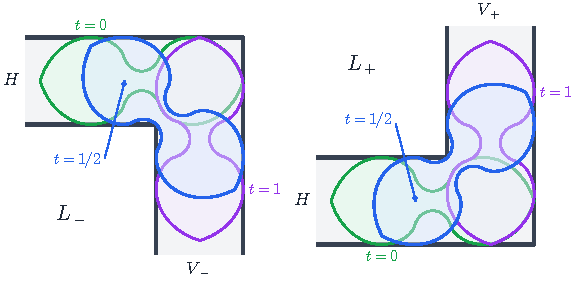
\includegraphics[width=\textwidth]{figures/fig-intro.pdf}
 \caption{Romik's sofa passing a right-turning corner (left) and a
 left-turning corner (right), from the same placement in the incoming
 arm. The illustrated motions turn through $-\pi/2$ and $\pi/2$,
 respectively.}\label{fig:intro}
\end{figure}

\subsection{Previous work}

Hammersley gave an early construction and the upper bound $2\sqrt2$ for
the ordinary problem \cite{Hammersley68}. Gerver constructed a sofa of
area $2.2195\ldots$ in 1992 \cite{Gerver92}, and Baek proved its
optimality \cite{Baek}. Requiring passage through both corners gives
a different extremal problem. The ambidextrous variant appears in
accounts of geometric problems \cite{CroftFalconerGuy91,Stewart04};
Gibbs obtained a numerical shape of area approximately $1.64495$
\cite{Gibbs14} before Romik found its exact description.

Romik derived differential equations for the contacts between a sofa
and the hallway walls, and solved them for the ambidextrous construction
\cite[Theorem~5]{Romik18}. Its boundary is piecewise algebraic, and
its area can be expressed by radicals and an inverse tangent. The
equations describe the construction within its contact pattern; they
do not give an upper bound for all admissible shapes and motions.
Kallus and Romik developed computer-assisted upper bounds for the
moving sofa problem \cite{KallusRomik18}. O'Keefe gives upper bounds
for its ambidextrous variant \cite{OKeefe26}, and Georgiev,
G\'omez-Serrano, Tao and Wagner list the ambidextrous problem as
Problem~6.63 \cite{GGTW25}.

We use Baek's theorem only to bound the areas of two auxiliary
ordinary sofas that occur in strict exclusions. The form needed here
is the rational upper bound $2.2199$; \cref{app:ordinary-sofa}
states this input and explains why it applies to those bodies.

\subsection{The strategy of the optimality proof}\label{sec:strategy-optimality}

Place the incoming sofa in the strip
$\Strip=\R\times[0,1]$. Its convex hull determines two downward
convex caps, $U$ and $V$: the upper hull boundary is the roof of $U$,
and reflecting the lower hull boundary in the midline gives the roof
of $V$. Each passage cuts a niche out of that hull. We must bound the
exterior roof area left after paying for the middle niche. At a
maximum, moving a supporting wall balances those two areas; the balance
then constrains the boundary curvature. This gives the following steps.

\begin{enumerate}[label=(\arabic*)]
 \item \emph{Pass from the actual motions to two cap scores.}
 Unless $|S|\le\sqrt2$, each passage supplies an effective turning
 angle in $(\pi/4,\pi/2]$. Let these angles be $\alpha$ and $\gamma$.
 The intermediate value theorem supplies every intervening hallway
 frame, even if the passage reverses its rotation. For a cap with
 projection $I$ and middle half $J$, define
 \[
  P_\alpha(U)=\int_{I\setminus J}f_U
                    -\int_J N_\alpha(U).
 \]
 Here $f_U$ is its roof and $N_\alpha(U)$ is the lower barrier imposed
 by the turn. The score counts the roof over the exterior quarters
 and subtracts the barrier over the middle half. An exact partition
 of vertical fibers gives
 \[
  |S|\le P_\alpha(U)+P_\gamma(V)
  \qquad\text{(\cref{sec:reduction}).}
 \]
 \item \emph{Obtain geometric laws for every maximizing cap.}
 After a horizontal translation, competitive caps lie in a fixed
 rectangle, and the score is continuous under Hausdorff convergence.
 A maximizer therefore exists. Cutting its middle roof to the chord
 joining the two middle endpoints, then restoring height one,
 cannot decrease its score. We approximate each prescribed canonical
 maximizer by polygons selected with a penalty for moving away from
 it (\cref{sec:selection}). Moving one polygon side compares the
 exterior roof gained with the inner-wall region lost. Passing these
 inequalities to the prescribed limit gives curvature bounds and
 endpoint laws (\cref{sec:variations}).
 \item \emph{Classify the full-turn maximizers.}
 The variation laws first exclude a tilted middle chord and force the
 middle roof to be horizontal (\cref{sec:full-turn}). They then give
 enough control of the two boundary arcs to identify the cap score
 with a functional of its support coordinates. A strict quadratic
 estimate and the equations of its stationary profiles show that
 this functional is at most $\Mc/2$, with equality only at Romik's
 support profile (\cref{sec:calibration}).
 \item \emph{Exclude equality at every proper turning angle.}
 If $\alpha<\pi/2$, the final outgoing strip imposes its first inner
 wall over the whole projection. This wall is part of $N_\alpha$,
 even where it rises above the swept niche. A variation bounds the
 length of the middle interval where this terminal wall is exposed.
 A weighted estimate for the opposite boundary arc forces that
 exposed interval to be longer, giving a contradiction
 (\cref{sec:partial-turn}). Thus $P_\alpha(U)\le\Mc/2$ for all
 angles under consideration, and equality requires a full turn.
\end{enumerate}

The small-area alternative satisfies $\sqrt2<\Mc$. In the other
case, steps (1), (3), and (4) give
\begin{equation}\label{eq:proof-chain}
 |S|\le P_\alpha(U)+P_\gamma(V)
     \le\frac\Mc2+\frac\Mc2=\Mc.
\end{equation}
The construction and exact area calculation in \cref{app:romik}
show that the upper bound is attained.

\subsection{The strategy of the uniqueness proof}\label{sec:strategy-uniqueness}

Suppose $|S|=\Mc$. Each inequality in \eqref{eq:proof-chain} is
then an equality. It follows that both original caps maximize their
scores. To identify $S$, the cap classification must apply to these
particular caps. The existence of a favorable maximizer would not
suffice: selecting a different maximizer, or replacing a middle roof
by its chord, can lose the information about the body that produced it.

This is why step (2) uses a penalty to select a prescribed cap. The
variation laws hold for every canonical maximizer, so the strict
support-function estimate identifies each one. The equality terms in
the chord cut and height restoration then recover the cap before
those operations. For a proper angle, the terminal-wall contradiction
is likewise applied to the prescribed maximizing pair $(\alpha,U)$.
Consequently equality in a cap score holds precisely when its angle
is $\pi/2$ and its cap is a horizontal translate of $\KR$.

The two caps of $S$ have the same projection. Their translates of
$\KR$ therefore align, and their intersection, after reflecting the
second cap, is a translate of Romik's hull. The original passage
constraints put $S$ inside the corresponding translate of $\SR$.
Equal area first gives equality up to a null set. Since $S$ is closed
and $\SR$ is the closure of its interior, a missing point would leave
a nonempty open subset of the interior missing as well, of positive
area. Thus the two compact sets are equal
(\cref{sec:equality,sec:recovery}). Applying this argument to any
witnessing pair of motions also forces each of its effective angles
to be $\pi/2$, proving the angular conclusion of \cref{thm:main}.

\subsection{Organization}

\Cref{sec:setting} defines the hallways, passages, caps, and scores.
\Cref{sec:reduction} proves the reduction from the two actual motions.
\Cref{sec:selection,sec:variations} obtain the approximation and
variation laws used by the analytic proof. \Cref{sec:full-turn,sec:calibration}
classify full-turn maximizers, and \cref{sec:partial-turn} proves the
universal cap bound and its strictness at proper angles.
\Cref{sec:equality} proves optimality and determines both equality
caps; \cref{sec:recovery} recovers the original compact body and proves
the quarter-turn conclusion. \Cref{sec:questions} gives further questions.

\Cref{app:ordinary-sofa} records the ordinary-sofa result used in
two exclusions. \Cref{app:romik} describes Romik's sofa, proves its
two explicit passages, and calculates its exact area.
\Cref{app:full-turn-estimates} proves the support-integral identities
and contact-energy estimates used for a full turn;
\cref{sec:variation-estimates} supplies the low-height exclusion.
\Cref{app:partial-turn-estimates} contains the initial-angle, circle,
and reflected-support estimates for the terminal tail.
\Cref{app:horizontal-estimates} gives the width and curvature estimates
for a horizontal middle, and \cref{app:preliminary-estimates} gives
the preliminary width and tilt bounds. Finally,
\cref{app:tilted-selector} excludes the remaining tilted configurations.

\section{Hallways, motions, and cap scores}\label{sec:setting}\label{sec:definitions}

We use $\abs{A}$ for two-dimensional Lebesgue measure and
$R_\theta$ for counterclockwise rotation by $\theta$. Put
\[
 u(\theta)=(\cos\theta,\sin\theta),\qquad
 u^\perp(\theta)=(-\sin\theta,\cos\theta),\qquad
 \refl(x,y)=(x,1-y).
\]
The reflection $\refl$ preserves the strip $\Strip=\R\times[0,1]$.

\begin{lemma}[Elementary bounds for the reference constant]\label{lem:constant-bounds}
The root and constant in \cref{eq:constant} satisfy
\[
 \frac{297}{1000}<Y<\frac3{10},\qquad
 \sqrt2<\frac85<\frac{41}{25}<\Mc.
\]
\end{lemma}
\begin{proof}
The polynomial $4y^3+3y$ is strictly increasing. Substitution at
$297/1000$ gives $248948073/250000000<1$, while its value at
$3/10$ is greater than one. For $y\ge0$,
$\arctan y\ge y-y^3/3$, since the derivative of
$\arctan y-y+y^3/3$ is $y^4/(1+y^2)\ge0$.
Using the cubic to replace $Y^3$ therefore gives
\[
 \Mc\ge\frac{11}{12}+4Y^2+\frac54Y
  >\frac{11}{12}+4(297/1000)^2+\frac54(297/1000)
  >\frac{41}{25}.
\]
The last inequality is rational arithmetic. The other comparisons
follow by squaring the positive quantities and comparing fractions.
\end{proof}

\subsection{The two passages}
The incoming and outgoing arms are
\begin{align*}
 \Hin&=(-\infty,1]\times[0,1],\\
 \Vm&=[0,1]\times(-\infty,1],&
 \Vp&=[0,1]\times[0,\infty).
\end{align*}
The two hallways are $\Lm=\Hin\cup\Vm$ and $\Lp=\Hin\cup\Vp$;
they are exchanged by $\refl$.

\begin{definition}\label{def:passage}
A passage of $S$ through $L=H\cup V$ consists of continuous maps
$\theta:[0,1]\to\R$ and $c:[0,1]\to\R^2$ such that
\[
 R_{\theta(0)}S+c(0)\subset H,\qquad
 R_{\theta(t)}S+c(t)\subset L\quad(0\le t\le1),\qquad
 R_{\theta(1)}S+c(1)\subset V.
\]
\end{definition}

\begin{definition}\label{def:ambidextrous}
An ambidextrous sofa is a nonempty compact connected set
$S\subset\R^2$ with a passage $(\theta_-,c_-)$ through $\Lm$ and
a passage $(\theta_+,c_+)$ through $\Lp$ satisfying
$R_{\theta_-(0)}=R_{\theta_+(0)}$.
\end{definition}

There is no smoothness assumption on $S$ or on either passage. The
continuous angle lifts may differ initially by an integer multiple of
$2\pi$. Compactness makes area finite, and connectedness refers to the
physical body, including its boundary. Initial translations need not
agree: translating a placement farther along the incoming arm does
not change its orientation.

\subsection{Caps and their roofs}
For a nonempty compact set $K$ define its support function by
\[
 h_K(\theta)=\max_{p\in K}\ip{p}{u(\theta)}.
\]
It is unchanged by taking the convex hull. For $K\subset\Strip$ let
\[
 K^\downarrow=\{(x,y):0\le y\le y'
              \text{ for some }(x,y')\in K\}.
\]

\begin{definition}\label{def:cap}
A downward cap is a nonempty compact convex set $U\subset\Strip$
such that $(x,y)\in U$ and $0\le y'\le y$ imply $(x,y')\in U$.
\end{definition}

Its horizontal projection is an interval $I_U=[l_U,r_U]$, its width
is $w_U=r_U-l_U$, and its roof is
\[
 f_U(x)=\max\{y:(x,y)\in U\}\quad(x\in I_U),
 \qquad f_U(x)=0\quad(x\notin I_U).
\]
On $I_U$ the roof is concave and takes values in $[0,1]$. The middle
half and exterior quarters are
\[
 J_U=[l_U+w_U/4,r_U-w_U/4],\qquad I_U\setminus J_U.
\]
The cap domain permits width zero, height less than one, flat faces,
and nonsmooth roofs. None of the later universal cap statements
assumes symmetry.

\subsection{The physical barrier}
Place a copy of $\Lm$ in the body's frame with its outer walls on
the supporting lines of $U$ with normals $u(\theta)$ and
$u^\perp(\theta)$. Its inner walls have heights
\begin{equation}\label{eq:walls}
 \begin{aligned}
 a_\theta(x)&=\frac{h_U(\theta)-1-x\cos\theta}{\sin\theta},\\
 b_\theta(x)&=\frac{h_U(\theta+\pi/2)-1+x\sin\theta}{\cos\theta}
 \qquad(0<\theta<\pi/2).
 \end{aligned}
\end{equation}
The forbidden open inner corner consists of points below both walls.
Its vertical threshold is $c_\theta(x)=\min(a_\theta(x),b_\theta(x))$.

For $0<\alpha\le\pi/2$ define the swept niche and full partial barrier
by
\begin{align}
 n_\alpha(U)(x)&=\max\left(0,\sup_{0<\theta<\alpha}c_\theta(x)\right),
       \label{eq:niche}\\
 N_\alpha(U)(x)&=\max\bigl(n_\alpha(U)(x),a_\alpha(x)\bigr).
       \label{eq:barrier}
\end{align}
The first-wall formula in \cref{eq:walls} remains defined at
$\alpha=\pi/2$. There
$a_{\pi/2}(x)=h_U(\pi/2)-1\le0$, so
$N_{\pi/2}(U)=n_{\pi/2}(U)$. At a proper terminal angle the outgoing
strip requires $y\ge a_\alpha(x)$ over the entire body, including
abscissae where that wall lies above the two-ray niche. This is why
the terminal wall appears separately in \cref{eq:barrier}.

\begin{lemma}[Continuity of the barrier]\label{lem:barrier-continuity}
For every downward cap $U$, $n_\alpha(U)$ and $N_\alpha(U)$
are continuous functions of $x$ for $\pi/4\le\alpha\le\pi/2$.
They are bounded and integrable on the cap's projection interval.
\end{lemma}
\begin{proof}
Set
\[
 \begin{aligned}
 m_U(x,t)&=\bigl(\min\{a_t(x),b_t(x)\}\bigr)_+
       &&(0<t<\pi/2),\\
 m_U(x,0)&=m_U(x,\pi/2)=0.
 \end{aligned}
\]
where $z_+=\max(z,0)$. On the open angular interval this is
continuous. At $t=0$, use
\[
 0\le m_U(x,t)\le
 \left(\frac{h_U(t+\pi/2)-1+x\sin t}{\cos t}\right)_+.
\]
The right side tends to zero, locally uniformly in $x$, because
$h_U(\pi/2)\le1$. At $t=\pi/2$ the analogous bound by
$(a_t(x))_+$ tends to zero. Thus $m_U$ is continuous on
$\R\times[0,\pi/2]$. Continuity at a proper terminal angle also
shows that
\[
 n_\alpha(U)(x)=\max_{0\le t\le\alpha}m_U(x,t).
\]
A continuous function's maximum over a compact interval depends
continuously on $x$: uniform continuity on any compact rectangle
bounds the difference of the two maxima by the largest difference
of the corresponding values. The terminal wall $a_\alpha$ is
continuous, since $\sin\alpha>0$, so taking its maximum with
$n_\alpha(U)$ proves the claim for $N_\alpha(U)$.
\end{proof}

\begin{figure}[htbp]
 \centering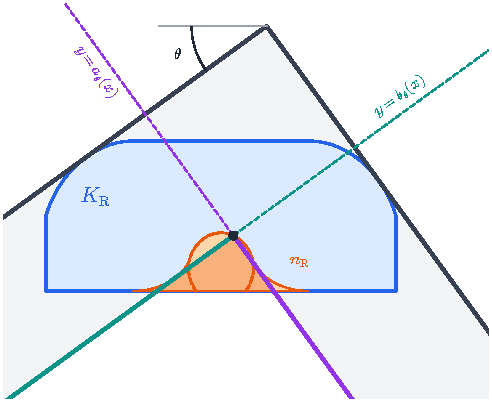
\includegraphics[width=.86\textwidth]{figures/fig-walls.pdf}
 \caption{The supporting hallway at $\theta=\pi/5$ for Romik's cap.
 The inner walls meet at its moving corner. The dashed corner path
 sweeps the niche as the angle varies.}\label{fig:walls}
\end{figure}

\begin{definition}\label{def:score}
The score of a cap at angle $\alpha$ is
\begin{equation}\label{eq:cap-score}
 P_\alpha(U)=\int_{I_U\setminus J_U}f_U(x)\,\dd x
              -\int_{J_U}N_\alpha(U)(x)\,\dd x.
\end{equation}
\end{definition}

The middle roof contributes no positive term to the score; its
support lines still affect the barrier. Both integration domains
move when the cap's projection changes. The elementary bound
\begin{equation}\label{eq:half-width}
 P_\alpha(U)\le w_U/2
\end{equation}
follows from $f_U\le1$, $N_\alpha(U)\ge0$, and
$\abs{I_U\setminus J_U}=w_U/2$.

\begin{figure}[htbp]
 \centering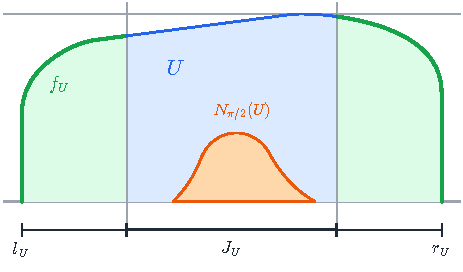
\includegraphics[width=.84\textwidth]{figures/fig-score.pdf}
 \caption{The score counts the roof over the two outer quarters
 (green) and subtracts the barrier over the middle half (orange).
 The cap drawn here is a generic cap, rather than Romik's.}\label{fig:score}
\end{figure}

\section{From continuous passages to two cap scores}\label{sec:reduction}

We first extract the angular information needed for the cap argument
from the two physical passages. The motions may reverse their direction
of rotation, and their terminal angles need not agree. Their initial
rotation maps agree, as required in the definition of an ambidextrous
sofa. Throughout this section the convex hull and both caps are formed
from the original body after one rigid change of coordinates.

\runin{Incoming normalization.}
Write the two placements as
\[
 g_\pm(t)p=R_{\vartheta_\pm(t)}p+v_\pm(t),\qquad 0\le t\le1.
\]
Set $T=g_-(0)S$. Both motions can be rebased to act on $T$ by
composing with $g_-(0)^{-1}$. Their continuous angle lifts can then be
chosen as $\vartheta_\pm(t)-\vartheta_\pm(0)$: equality of the initial
rotation maps suffices, even if the original lifts differ by an integer
multiple of $2\pi$. Thus $T\subseteq\Strip$, both rebased initial angles
are zero, and $|T|=|S|$. The rebased translations are allowed to differ.
Compactness and connectedness are preserved by this normalization.


\runin{Support tightening at a visited frame.}
For normals $u(\theta),u^\perp(\theta)$ and offsets $A,B$, write
\begin{equation}\label{eq:frame-hall}
 \begin{split}
 H_\theta(A,B)=\{p:\ &\ip{p}{u(\theta)}\le A+1,
                  \ \ip{p}{u^\perp(\theta)}\le B+1,\\
                  &\ip{p}{u(\theta)}\ge A\ \text{or}\
                   \ip{p}{u^\perp(\theta)}\ge B\}.
 \end{split}
\end{equation}
If this hallway contains $T$, then, for $K=\conv T$,
\[
 h_K(\theta)-1\le A,\qquad h_K(\theta+\pi/2)-1\le B.
\]
Replace $A,B$ by those support offsets. Both outer walls still
contain $K$, and each inner alternative becomes weaker. Consequently
\begin{equation}\label{eq:support-tightening}
 T\subseteq H_\theta\bigl(h_K(\theta)-1,h_K(\theta+\pi/2)-1\bigr).
\end{equation}
This argument retains $T$; it makes no assertion that the nonconvex
hallway contains its entire convex hull.
Continuity of $h_K$ makes these tightened placements continuous when
the frame angle varies continuously.

\begin{lemma}[The effective angle]\label{lem:effective-angle}
Let $T\subseteq\Strip$ be nonempty and compact, with $|T|>\sqrt2$.
For any normalized passage through $\Lm$, there is
$\alpha\in(\pi/4,\pi/2]$ with the following properties:
every angle in $[0,\alpha]$ occurs as a body-relative hallway frame;
$T$ satisfies the support-tightened hallway constraints at every
interior angle; and
\begin{equation}\label{eq:effective-terminal-wall}
 h_K(\alpha)-1\le\ip{p}{u(\alpha)}\quad\text{for every }p\in T.
\end{equation}
Moreover, either the passage reaches a clockwise quarter turn and
$\alpha=\pi/2$, or $\alpha$ is the clockwise magnitude of its actual
terminal angle and $\alpha<\pi/2$.
\end{lemma}

\begin{proof}
Let $\vartheta$ be the rebased body angle and put
$\theta(t)=-\vartheta(t)$, the hallway frame angle, so that
$\theta(0)=0$. First exclude the wrong frame $-\pi/4$.
The two outer inequalities have normals $(1,-1)/\sqrt2$ and $(1,1)/\sqrt2$.
For arbitrary offsets $A,B$, the horizontal section of
\eqref{eq:frame-hall} at ordinate $y$ is
\[
 [m(y),m(y)+\sqrt2],\qquad
 m(y)=\min\{\sqrt2 A+y,\sqrt2 B-y\}.
\]
Indeed the inner alternatives say that $x$ is at least one of the
two displayed affine expressions, and the two outer walls say that
$x$ is at most each of those expressions plus $\sqrt2$.
Intersecting with $0\le y\le1$ gives area at most $\sqrt2$.
The body therefore cannot visit this frame. Continuity also excludes
every smaller frame angle: reaching one would first require visiting
$-\pi/4$.

The actual outgoing arm at time $1$ puts the whole body into a unit
strip normal to $u(\theta(1))$. If
$-\pi/4<\theta(1)\le\pi/4$, its intersection with $\Strip$ has
area $1/\cos\theta(1)\le\sqrt2$. To see this directly, a strip
$A\le x\cos\theta+y\sin\theta\le A+1$ has, at each fixed
$y$, a horizontal section of length $1/\cos\theta$.
Thus $\theta(1)>\pi/4$.

If the lift reaches $\pi/2$, take $\alpha=\pi/2$. Otherwise
continuity forces $\theta(1)<\pi/2$, and we take
$\alpha=\theta(1)$. The intermediate value theorem supplies every
angle between zero and $\alpha$ in either case. Applying
\eqref{eq:support-tightening} at those times proves the interior
hallway constraints, with no assumption that the original motion is
monotone.

For a proper terminal angle the actual outgoing strip gives
\eqref{eq:effective-terminal-wall}: its lower offset is at least
$h_K(\alpha)-1$. In the full-angle case it follows
from the incoming strip alone, because $u(\pi/2)=(0,1)$,
$h_K(\pi/2)\le1$, and $y\ge0$ on $T$.

\end{proof}

Apply the lemma independently to the lower passage and to the
reflection of the upper passage across $y=1/2$. Reflection reverses
the lifted body angle and changes $\Lp$ into $\Lm$; it preserves
area. We obtain angles
\begin{equation}\label{eq:effective-angles}
 \frac\pi4<\alpha\le\frac\pi2,\qquad
 \frac\pi4<\gamma\le\frac\pi2.
\end{equation}
If an angle is proper, its terminal wall comes from its own passage.
The two passages need not have the same visited times or translations.


\runin{The caps of the actual hull.}
Let $I=[l,r]$ be the horizontal projection of $T$, and set $w=r-l$.
Connectedness makes this projection the whole interval $I$; taking
the convex hull adds no abscissas. Write its vertical fibers as
\[
 K_x=[B(x),A(x)]\quad(x\in I),
\]
and define the downward caps
\begin{equation}\label{eq:actual-caps}
 U=K^\downarrow,\qquad V=(\refl K)^\downarrow.
\end{equation}
Their roofs satisfy $f_U=A$ and $f_V=1-B$, and both caps have
projection $I$. In particular
\begin{equation}\label{eq:hull-from-caps}
 K=U\cap\refl V.
\end{equation}
The statements hold at the projection endpoints as well as in its
interior. The caps are nonempty compact convex subsets of $\Strip$.

\begin{figure}[t]
 \centering
 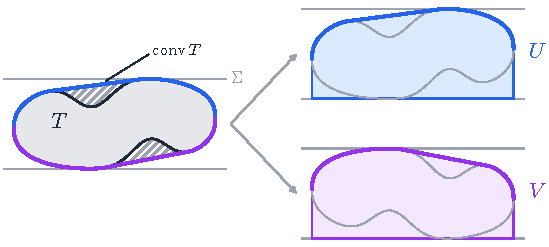
\includegraphics[width=.82\textwidth]{figures/fig-reduction.pdf}
 \caption{The original body $T$, its convex hull, and the two
 downward caps $U$ and $V$. The upper hull boundary is the roof of
 $U$; reflecting the lower hull boundary gives the roof of $V$.
 The hatched part illustrates area added by convexification.}
 \label{fig:reduction}
\end{figure}

Downward filling preserves support in every direction with
nonnegative vertical component. Since both $u(\theta)$ and
$u^\perp(\theta)$ point upwards for $0<\theta<\pi/2$, the
lower constraints of $T$ use exactly the supports of $U$. The
reflected upper constraints use those of $V$. Denote the resulting
barriers by
\[
 N_U=N_\alpha(U),\qquad N_V=N_\gamma(V).
\]
Each barrier includes the positive supremum of the two-wall minima
over the entire open angular interval and the terminal first wall
\[
 a_\alpha(x)=\frac{h_U(\alpha)-1-x\cos\alpha}{\sin\alpha}
\]
(with $V,\gamma$ for the other passage). This last wall is redundant
at a full quarter turn and is retained at every proper endpoint.
Thus every $(x,y)\in T$ satisfies $N_U(x)\le y$ and
$N_V(x)\le1-y$.



\runin{Physical fibers and the exact partition loss.}
Put $d_U=1-f_U$ and $d_V=1-f_V$. The actual four-wall envelope is
\begin{equation}\label{eq:physical-envelope}
 E=\left\{(x,y):x\in I,\quad
    \max\{d_V(x),N_U(x)\}\le y
    \le1-\max\{d_U(x),N_V(x)\}\right\}.
\end{equation}
We have $T\subseteq E$. Its signed fiber length is
\begin{equation}\label{eq:signed-length}
 \ell(x)=1-\max\{d_V(x),N_U(x)\}
             -\max\{d_U(x),N_V(x)\}.
\end{equation}
For arbitrary wall data, the actual length of that fiber is
$\ell(x)_+=\max\{\ell(x),0\}$. Here connectedness supplies a point
of $T$ at every $x\in I$, and containment supplies a point of $E$
in the same fiber. Consequently $\ell(x)\ge0$ everywhere on $I$,
and Cavalieri's formula gives
\begin{equation}\label{eq:envelope-area}
 |E|=\int_I\ell(x)\,\dd x\ge|T|.
\end{equation}
Compactness gives measurable roofs. The barriers are continuous by \cref{lem:barrier-continuity},
so all these functions are measurable and integrable on $I$.

Let $J=[l+w/4,r-w/4]=J_U=J_V$ be the middle half of $I$. Define
\begin{align}\label{eq:partition-defect}
 D_{\rm part}={}&
 \int_J\bigl[(d_V-N_U)_++(d_U-N_V)_+\bigr]\,\dd x\notag\\
 &+\int_{I\setminus J}
       \bigl[(N_U-d_V)_++(N_V-d_U)_+\bigr]\,\dd x.
\end{align}
It is nonnegative. The pointwise identity
$\max\{a,b\}-a=(b-a)_+$ yields
\[
 \begin{cases}
  1-N_U-N_V-\ell=(d_V-N_U)_++(d_U-N_V)_+,&x\in J,\\
  1-d_U-d_V-\ell=(N_U-d_V)_++(N_V-d_U)_+,&x\in I\setminus J.
 \end{cases}
\]
Since $|J|=|I\setminus J|=w/2$, the constant terms cancel on
integration. Recalling the score
\[
 P_\alpha(U)=\int_{I\setminus J}f_U\,\dd x
                         -\int_J N_U\,\dd x,
\]
we obtain the exact identity
\begin{equation}\label{eq:score-envelope-defect}
 P_\alpha(U)+P_\gamma(V)-|E|=D_{\rm part}.
\end{equation}

\begin{proposition}[Original-body score reduction]\label{prop:reduction}
Every ambidextrous sofa $S$ satisfies either $|S|\le\sqrt2$, or,
after an area-preserving rigid normalization, has the actual caps
$U,V$ and independent angles \eqref{eq:effective-angles} with
\begin{equation}\label{eq:two-cap-bound}
 |S|\le P_\alpha(U)+P_\gamma(V).
\end{equation}
More precisely, for every real comparison constant $c$,
\begin{equation}\label{eq:four-term-deficit}
 \begin{split}
 c-|S|={}&\left(\frac c2-P_\alpha(U)\right)
          +\left(\frac c2-P_\gamma(V)\right)\\
         &+D_{\rm part}+|E\setminus T|.
 \end{split}
\end{equation}
\end{proposition}

\begin{proof}
The small-area alternative is immediate. In the other case use the
normalization, effective-angle lemma, and actual cap constructions
above. The measurable bounded envelope contains $T$, so
$|E\setminus T|=|E|-|T|$. Substitute this into
\eqref{eq:score-envelope-defect}, then use $|T|=|S|$.
Dropping the two nonnegative geometric losses gives
\eqref{eq:two-cap-bound}.
\end{proof}

The scalar score in \cref{prop:reduction} is defined on every downward
cap, whether or not that cap arises from a feasible connected body.
The signed algebra also holds on that larger domain. The conversion
of $\int\ell$ into ordinary area used the actual body's connected
projection; it is needed only for the reduction from physical sofas.

\begin{remark}\label{rem:negative-fibers}
This distinction cannot be dropped for arbitrary convex hulls.
Take $K=[-1,1]\times[0,1]$ and both full angles. At $x=0$ the two
inner walls for $\theta=\pi/4$ have height $2-\sqrt2$.
Thus $N_U(0),N_V(0)\ge2-\sqrt2$, and
$\ell(0)\le2\sqrt2-3<0$. The central envelope fiber is empty.
The general area formula is $|E|=\int_I\ell_+\,\dd x$;
\eqref{eq:envelope-area} applies because the original connected body
certifies that every fiber is nonempty.
\end{remark}

\section{Selecting polygons near a prescribed maximum}\label{sec:selection}

Put $L=\pi/2$. A \emph{full maximum} is a cap maximizing $P_L$ over
all downward caps. A \emph{joint maximum} is a pair $(U,\alpha)$
maximizing $P_\alpha(U)$ over all caps and all $\alpha\in[L/2,L]$.
We shall construct polygons converging to any prescribed maximum.
This quantifier will also be needed in the equality argument.

\subsection{Compactness and continuity}

\begin{lemma}[Width bounds]\label{lem:selection-width}
If $P_\alpha(U)\ge M/2$ and $L/2\le\alpha\le L$, then
$M\le w_U<6$. After horizontal translation, $U$ lies in
$[-3,3]\times[0,1]$.
\end{lemma}

\begin{proof}
Since $f_U\le1$ and $N_\alpha(U)\ge0$, $P_\alpha(U)\le w_U/2$.
Center the projection and write $w=w_U$. The baseline endpoints give
$\sqrt2 h_U(L/2),\sqrt2 h_U(3L/2)\ge w/2$.
The two walls at $L/2$ therefore give
\[
 N_\alpha(U)(x)\ge(w/2-\sqrt2-|x|)_+.
\]
For $\alpha=L/2$ the terminal first wall dominates this minimum;
for larger $\alpha$ it is one of the visited two-wall minima.
If $w\ge6$, the displayed tent is positive on $[-w/4,w/4]$, and
\[
 P_\alpha(U)\le\frac{(1+\sqrt2)w}{2}-\frac{3w^2}{16}.
\]
This quadratic decreases for $w\ge6$. Its value at six is
$3\sqrt2-15/4<3/4<M/2$, a contradiction. Centering a cap of
width less than six gives the asserted box.
\end{proof}

\begin{lemma}[Continuity of the score]\label{lem:selection-continuity}
On the space of nonempty downward caps in a fixed bounded box,
$P_\alpha(U)$ is jointly continuous in Hausdorff distance and in
$\alpha\in[L/2,L]$.
\end{lemma}

\begin{proof}
Take the box $[-B,B]\times[0,1]$. Its support functions are uniformly
bounded and uniformly Lipschitz in angle. For $x\in[-B,B]$,
\begin{equation}\label{eq:selection-tails}
 (\min(a_t(x),b_t(x)))_+\le2B\min(\tan t,\cot t),\qquad
 (a_\alpha(x))_+\le2B\cot\alpha.
\end{equation}
For example $h_U(t+L)\le B\sin t+\cos t$, so
$b_t(x)\le(B+x)\tan t+1-\sec t\le2B\tan t$.
The first wall gives the other tail bound and the terminal bound.

If two cap supports differ by at most $\eta$, their walls differ by
at most $\eta/\sin\delta$ on $[\delta,L-\delta]$.
The omitted positive tails are at most $2B\tan\delta$. Taking
maxima and minima preserves these estimates. Thus the full niche
changes by at most
\[
 4B\tan\delta+\frac{\eta}{\sin\delta}.
\]
For a varying endpoint below $L$, first restrict to a closed angular
interval away from the axes. Uniform continuity there controls both
the support change and the change of its upper limit. At $\alpha=L$
the second estimate in \eqref{eq:selection-tails} makes the positive
terminal wall tend uniformly to zero. Hence the complete barriers
converge uniformly on the horizontal box.

Projection endpoints converge because they are horizontal supports.
The roofs converge in $L^1$: Hausdorff convergence of bounded convex
sets gives convergence of their indicators almost everywhere away
from the limiting boundary, and integrating the vertical fibers gives
the roof assertion. If the limit is degenerate, the approximating
convex-set areas tend to zero and the same conclusion follows.
The symmetric difference of the moving middle intervals has length
tending to zero. Bounded roofs and barriers now give convergence of
both integrals defining the score.
\end{proof}

\begin{proposition}[Attainment]\label{lem:selection-maximum}
Full and joint maxima exist. A joint maximum can be chosen with its
angle largest among all joint maximizing angles.
\end{proposition}

\begin{proof}
The reference cap has $P_L(\KR)=M/2$. By
\cref{lem:selection-width}, every competitor at least this good can
be centered in $[-3,3]\times[0,1]$. Blaschke's compactness theorem
applies to the nonempty compact convex subsets of this box. Their
downward closure is preserved under Hausdorff limits: approximate
$(x,y)$ by $(x_n,y_n)$ and lower its ordinate to
$\min(y',y_n)$ for $0\le y'\le y$.
The score continuity lemma therefore gives a maximum in the box,
both with $\alpha=L$ fixed and with $\alpha\in[L/2,L]$ variable.
Width bounds remove the box restriction from the conclusion.
The joint maximizing level set is compact; maximize its angle
coordinate to obtain the final assertion.
\end{proof}

\subsection{Canonicalization and used supports}

\begin{lemma}[Chord and height reduction]\label{lem:selection-canonical}
For any positive-width cap $U$ and fixed $0<\alpha\le L$, there
is a cap $U^\sharp$ with the same projection, height one, and an
affine roof on $J_U$, such that $P_\alpha(U^\sharp)\ge P_\alpha(U)$.
Applied to a full or joint maximum, the construction preserves its
score and its angle.
\end{lemma}

\begin{proof}
Let $q$ join the roof values at the endpoints $j_-,j_+$ of $J_U$.
Concavity gives $f_U\ge q$ on $J_U$ and $f_U\le q$ outside it.
For the latter assertion, write $j_-$ as a convex combination of
$x<j_-$ and $j_+$ and solve the concavity inequality for $f_U(x)$;
the right side follows by exchanging endpoints. In particular
$q\ge0$ throughout the projection.
The cap $U^{\rm c}=U\cap\{y\le q(x)\}$ therefore has the same
projection and exterior roof. Inclusion decreases every support,
hence every visited wall and the terminal first wall. Its barrier
decreases, so its score increases.

If $H$ is the height of $U^{\rm c}$, put $\varepsilon=1-H$ and
$U^\sharp=U^{\rm c}+[0,\varepsilon]e_y$.
Its roof rises by $\varepsilon$. Supports in the two visited
families rise by $\varepsilon\sin t$ and $\varepsilon\cos t$;
both raw walls, including the terminal wall, rise by exactly
$\varepsilon$. The maximum with the floor gives
\[
 0\le N_\alpha(U^\sharp)-N_\alpha(U^{\rm c})\le\varepsilon.
\]
The exterior and middle intervals have equal length, so the exterior
gain pays this middle penalty. The projection stays fixed, the
middle roof stays affine, and the height becomes one. Maximality
forces equality of scores when the starting cap is a maximum.
\end{proof}

We call a height-one cap with affine middle roof \emph{canonical}.
Write $f_U(x)=mx+c$ on its middle interval and let $\theta_c$ be
the normal angle of this facet, so $\cot\theta_c=-m$.

\begin{lemma}[Top localization]\label{lem:selection-top}
At every positive full or joint maximum the top face meets $J_U$.
For a canonical maximum the higher middle endpoint has height one.
\end{lemma}

\begin{proof}
Suppose the top face starts at $a>j_+$. Adjoin $(j_+,H)$ and its
downward segment, and take the convex hull. A changed upward support
must have negative horizontal component, because the old top point
$(a,H)$ dominates the new point in all other directions. Its new
support is $\ip{(j_+,H)}{n}$; for $x\in J_U$ and $y\ge0$,
\[
 \ip{(j_+,H)-(x,y)}{n}-1
 =(j_+-x)n_x+(H-y)n_y-1\le0.
\]
Thus changed second walls contribute no positive niche on $J_U$;
first walls and the terminal wall are unchanged. The barrier is
unchanged, whereas the exterior roof strictly increases on
$(j_+,a)$. If the top lies left of $J_U$, insert $(j_-,H)$.
Changed supports then have positive horizontal component and the
same inequality makes their first walls, including the terminal
wall, nonpositive on $J_U$. Both cases contradict maximality.
\end{proof}

\begin{lemma}[Saturation]\label{lem:selection-saturation}
For a canonical joint maximum $(U,\alpha)$,
\begin{equation}\label{eq:selection-saturation}
 \begin{gathered}
 U=U^{\rm sat}\cap\{y\le mx+c\},\\
 U^{\rm sat}=(I_U\times[0,1])\cap
 \bigcap_{0\le t\le\alpha} H_t,\\
 H_t=\{z:\ip z{u(t)}\le h_U(t),\
             \ip z{u^\perp(t)}\le h_U(t+L)\}.
 \end{gathered}
\end{equation}
On either unused open normal arc $(\alpha,L)$ or $(L+\alpha,\pi)$,
the upper curvature measure is zero except possibly at $\theta_c$.
Thus the support is harmonic on the unused arcs away from that normal.
\end{lemma}

\begin{proof}
The saturated cap contains $U$, retains its baseline, and has the
same support in each used direction: its defining inequalities give
one bound and inclusion gives the opposite bound. In particular it
has the same height and complete barrier. Maximality makes its
exterior roof equal to $f_U$, since a strict increase at an interior
exterior point would increase an area integral. Continuity gives
equality at $j_\pm$; cutting to their chord now proves
\eqref{eq:selection-saturation}.
Every boundary point of $U^{\rm sat}$ has an active constraint from
the compact family of defining normals. At arclength almost every
boundary point its outer normal is unique, so equals an active
normal. There is consequently no surface-area measure on unused
open arcs. The chord cut only adds its facet normal $\theta_c$.
The distributional identity $h''+h=0$ on the remaining arcs is the
stated harmonicity.
\end{proof}

\subsection{A penalty that retains any chosen maximum}

Fix a full maximum $U_*$, or a joint maximum $(U_*,\alpha)$ and
keep this angle fixed. Choose a horizontal box with unit slack
beyond both projection endpoints. For $n=2^k$ set
$t_j=j\alpha/n$ and use the sampled barrier
\[
 N_{k,\alpha}(V)=\max\{0,
       \max_{0<j<n}\min(a_{t_j},b_{t_j}),a_\alpha\}.
\]
For $\alpha=L$ the last wall is redundant. Let $P_{k,\alpha}$ be
the corresponding score. Sample outer normals on the two source
grids and on an independent dyadic grid of the whole upper semicircle:
\[
 \Gamma_k=\{jL/n:0\le j\le2n\}
       \cup\{t_j,L+t_j:0\le j\le n\}.
\]
These sets are nested, contain the axes and top, and have dense union.

\begin{lemma}[Uniform grid error and circumscription]\label{lem:selection-grid}
On the fixed boxed cap domain,
\[
 0\le P_{k,\alpha}(V)-P_\alpha(V)\le e_k,
 \qquad e_k\longrightarrow0.
\]
Circumscription by the normals $\Gamma_k$ preserves every sampled
support, projection, and sampled barrier, and increases the exterior
roof. It therefore increases $P_{k,\alpha}$.
\end{lemma}

\begin{proof}
On $[\delta,L-\delta]$ the wall functions have a common modulus of
continuity in angle. A mesh of size $\alpha/2^k$ approximates their
maximum uniformly there. Equation \eqref{eq:selection-tails} makes
the omitted endpoint contributions uniformly small. The terminal
wall is already included exactly. First choose $\delta$ and then
the mesh; this gives uniform barrier approximation. Multiplying
its error by the bounded middle length proves the score estimate.
The circumscribed intersection contains the original cap and retains
each sampled support: an old attaining point remains in it, and the
corresponding defining halfplane gives the upper bound. The axis
supports preserve the projection, and all barrier supports are sampled.
\end{proof}

For $s\in\Gamma_m$ give its level-$m$ sample weight
$\nu_m=2^{-m-1}/|\Gamma_m|$, and define the persistent penalty
\begin{equation}\label{eq:selection-penalty}
 D_k(V,U_*)=\sum_{m=0}^k\nu_m\sum_{s\in\Gamma_m}
                   (h_V(s)-h_{U_*}(s))^2.
\end{equation}
The total weight is at most one. A normal first sampled at an early
level keeps that positive weight at every later level. In particular
\begin{equation}\label{eq:selection-persistence}
 \nu_m(h_V(s)-h_{U_*}(s))^2\le D_k(V,U_*)
 \quad(s\in\Gamma_m,\ m\le k).
\end{equation}

\begin{theorem}[Selection at a prescribed maximum]\label{thm:selection-prescribed}
There are levels $k_i\to\infty$, coefficients $\eta_i\downarrow0$,
and grid polygons $U_i$ converging in Hausdorff distance to the
specified cap $U_*$, such that $U_i$ maximizes
\[
 P_{k_i,\alpha}(V)-\eta_iD_{k_i}(V,U_*)
\]
over every cap in the slack box. No middle affinity or regularity
is required of the selected polygons.
\end{theorem}

\begin{proof}
Choose $\eta_i=1/(i+1)$ and $k_i\ge i$ so that $e_{k_i}\le\eta_i^2$.
Compactness and continuity give a boxed maximum of the penalized
objective. Circumscription increases its score and preserves its
penalty, so a maximizing cap can be taken to be a grid polygon.
The circumscription of $U_*$ has zero penalty and sampled score at
least $P_\alpha(U_*)$. Hence
\[
 P_\alpha(U_*)\le P_{k_i,\alpha}(U_i)-\eta_iD_{k_i}(U_i,U_*)
 \le P_\alpha(U_*)+e_{k_i}-\eta_iD_{k_i}(U_i,U_*),
\]
where the second inequality uses the maximality of $U_*$ at its
fixed angle. Thus $D_{k_i}(U_i,U_*)\le\eta_i\to0$.
Any Hausdorff cluster cap has, by \eqref{eq:selection-persistence},
the same support as $U_*$ at every sampled normal. Density gives
equality on the upper semicircle. For a downward cap, downward
supports are determined by its baseline and horizontal endpoints;
the upper supports consequently determine the entire cap. Every
cluster cap is $U_*$, which proves convergence of the whole sequence.
Its artificial box sides are inactive for all sufficiently large $i$.
\end{proof}

If all support values have absolute value at most $B$, changing
sampled supports by at most $r$ changes the penalty by at most
$4Br+r^2$. If only one normal changes, multiply this bound by its
total persistent weight. These bounds tend to zero after multiplication
by $\eta_i$ and will account for the error in the polygon variations.

\section{Facet variations and limiting source laws}\label{sec:variations}

Fix a prescribed canonical full maximum, or a canonical joint maximum
$(U,\alpha)$ with $\alpha<L$. Use the selections of
\cref{thm:selection-prescribed}. Write $U_i$ for a selected polygon,
$h_i$ for its support, $A_i=f_{U_i}$, and $q_i$ for its sampled
complete barrier. Its projection and middle interval are $I_i,J_i$.
All supports are bounded by $B$ in absolute value, the mesh tends
to zero, and the penalty coefficient $\eta_i$ tends to zero.
We take each polygonal variation first, with $i$ fixed.

\subsection{Moving a floating side and an endpoint}

For a nonaxis, nontop sampled normal $s$, let $\ell_{i,s}$ be the
outer facet length, $\ell^{\rm w}_{i,s}$ its part over
$I_i\setminus J_i$, and $\ell^{\rm m}_{i,s}$ its part over $J_i$.
Let $\tau_{i,s}$ be the length of the positive barrier graph over
$J_i$ carried by the inner line with this normal. The terminal first
line is counted when $\alpha<L$; an unused normal has $\tau_{i,s}=0$.
Distinct source lines have distinct slopes, so their intersection
points do not create ambiguity in these lengths.

\begin{lemma}[Finite facet variation]\label{lem:variation-finite}
With $w_{i,s}$ the total persistent weight at $s$, put
$b_{i,s}=4B\eta_iw_{i,s}$ and $\beta_i=\sum_s b_{i,s}\le4B\eta_i$.
Then
\begin{equation}\label{eq:variation-facet}
 \ell^{\rm w}_{i,s}\le\tau_{i,s}+b_{i,s}.
\end{equation}
At a positive vertical end face the outward derivatives of the
unpenalized score are $e_{i,R}-C_{i,R}$ and $e_{i,L}-C_{i,L}$, where
\begin{equation}\label{eq:variation-pressures}
 \begin{gathered}
 Q_{i,\pm}=A_i(j_{i,\pm})+q_i(j_{i,\pm}),\\
 C_{i,R}=(3Q_{i,+}-Q_{i,-})/4,\qquad
 C_{i,L}=(3Q_{i,-}-Q_{i,+})/4,\\
 e_{i,R}=A_i(r_i),\qquad e_{i,L}=A_i(l_i).
 \end{gathered}
\end{equation}
For all end faces, including zero ones,
\begin{equation}\label{eq:variation-endpoint-upper}
 e_{i,R}\le(C_{i,R}+b_{i,0})_+,\qquad
 e_{i,L}\le(C_{i,L}+b_{i,\pi})_+.
\end{equation}
\end{lemma}

\begin{proof}
Move the supporting line at $s$ outwards by $\varepsilon>0$, keeping
all other grid halfplanes. An old attaining point remains for each
unchanged support, so those supports stay fixed. For a positive
facet the moved support rises by $\varepsilon$ for sufficiently
small $\varepsilon$. The projection and $J_i$ are unchanged.
The gained outer strip has area
$\varepsilon\ell^{\rm w}_{i,s}+O(\varepsilon^2)$. The gained
forbidden area has area
$\varepsilon\tau_{i,s}+O(\varepsilon^2)$: an exposed inner
segment moves by its normal displacement, and finitely many line
intersections, floor contacts, and window endpoints contribute
quadratic errors. Thus the score derivative is
$\ell^{\rm w}_{i,s}-\tau_{i,s}$. The penalty derivative has absolute
value at most $b_{i,s}$. Maximality gives
\eqref{eq:variation-facet}; at zero facet length it is automatic.

Move a positive right end face from $r_i$ to $r_i+\varepsilon$.
Nonaxis supports and $q_i(x)$ stay fixed, whereas the middle
endpoints move by $\varepsilon/4,3\varepsilon/4$. Differentiating
the three integrals gives
\[
 e_{i,R}+\tfrac14(A_i+q_i)(j_{i,-})
          -\tfrac34(A_i+q_i)(j_{i,+})=e_{i,R}-C_{i,R}.
\]
Moving the left face outwards moves the middle endpoints by
$-3\varepsilon/4,-\varepsilon/4$ and gives $e_{i,L}-C_{i,L}$.
If an end face has height zero, its retained last sloping halfplane
and the floor already impose the endpoint. Relaxing the axis
constraint then leaves the body unchanged. This proves precisely
the positive-part bounds \eqref{eq:variation-endpoint-upper}.
\end{proof}

\subsection{The four neighboring lines}

\begin{lemma}[Neighbor exposure]\label{lem:variation-neighbors}
At an interior first source $t$ with source spacing $\delta$, put
$f=h_i(t)$, $g=h_i(t+L)$, $c=\cos\delta$, $s=\sin\delta$,
and $T=\tan(\delta/2)$. Let
\[
 \ell^{\rm circ}=
 \frac{h_i(t-\delta)+h_i(t+\delta)-2cf}{s}\ge0.
\]
The full exposed first-wall length satisfies
\begin{equation}\label{eq:variation-neighbor}
 \tau\le\tan\delta(|q^+|+T)+(2T-\ell^{\rm circ})_+,
 \qquad q^+=f+\frac{h_i(t+L+\delta)-cg}{s}-1.
\end{equation}
The corresponding second-source bound has the roles of the two
normal families interchanged.
\end{lemma}

\begin{proof}
Parameterize the first inner ray by
$z(v)=(f-1)u(t)+v u^\perp(t)$, $v\le v_0=g-1$.
To avoid both neighboring open quadrants, an exposed point must lie in
\[
 [\min(v_-,v_+),v_0]\ \cup\ [v_{\rm lo},v_{\rm hi}],
\]
where solving the four neighboring line inequalities gives
\[
 \begin{aligned}
 v_-&=\frac{h_i(t+L-\delta)-1-(f-1)s}{c},&
 v_+&=\frac{h_i(t+L+\delta)-1+(f-1)s}{c},\\
 v_{\rm lo}&=\frac{h_i(t+\delta)-1-(f-1)c}{s},&
 v_{\rm hi}&=\frac{(f-1)c-h_i(t-\delta)+1}{s}.
 \end{aligned}
\]
Indeed either a neighboring companion alternative holds, putting
the point in the first interval, or both neighboring first alternatives
must hold, putting it in the second. At zero the neighboring quadrant
is below the floor; at a proper terminal endpoint it is dominated
by the whole terminal first wall. These neighbors remain valid.
Subtracting gives $v_{\rm hi}-v_{\rm lo}=2T-\ell^{\rm circ}$.
If $d_-=(gc-h_i(t+L-\delta))/s$ and
$d_+=(h_i(t+L+\delta)-gc)/s$, then $d_-\le d_+$ and
\[
 v_0-v_-=\tan\delta(f+d_--1+T),\qquad
 v_0-v_+=\tan\delta(-q^++T).
\]
The first interval therefore has length at most
$\tan\delta(|q^+|+T)$. Floor clipping only shortens the exposed
pieces, proving the bound. The second-source calculation is the
same calculation in the interchanged orthonormal coordinates.
\end{proof}

In a full grid $\ell^{\rm circ}=\ell_{i,t}$; with additional
outer normals $\ell_{i,t}\le\ell^{\rm circ}$. Uniform support
and support-slope bounds imply, for a fixed constant $K$,
\begin{equation}\label{eq:variation-coarse}
 \tau_{i,t},\tau_{i,t+L}\le K\delta,
 \qquad
 \ell_{i,s}\le K\delta+b_{i,s}+\ell^{\rm m}_{i,s}
\end{equation}
at nonterminal source normals. Normals used only for circumscription
satisfy $\ell^{\rm w}_{i,s}\le b_{i,s}$.
The terminal first source instead satisfies
$\tau_{i,\alpha}\le |J_i|/\sin\alpha$; this mass is retained.
There is no terminal companion source, since its two-wall minimum
is dominated by the terminal first wall.

\begin{lemma}[Vanishing middle errors]\label{lem:variation-middle}
On every compact normal arc separated from $\theta_c$ and $L$,
$\sum_s\ell^{\rm m}_{i,s}\to0$.
\end{lemma}

\begin{proof}
Concavity and the bound $0\le A_i\le1$ give uniform roof-slope
bounds near $J_U$, because this interval stays a positive distance
from the projection endpoints. The roofs converge uniformly there.
On $[j_-+\varepsilon,j_+-\varepsilon]$, their one-sided slopes
converge uniformly to the middle slope $m$: bound each derivative
between its two secant slopes to points a fixed distance away and
then pass to the uniform limit. Thus every middle facet there has
normal arbitrarily close to $\theta_c$. The two remaining boundary
strips have total arclength at most a fixed constant times
$\varepsilon+o(1)$. Let $i\to\infty$ and then
$\varepsilon\downarrow0$.
\end{proof}

\begin{lemma}[The tilted middle junctions]\label{lem:variation-middle-junctions}
If a canonical full or joint maximum has $m\ne0$, then
$A'_-(j_-)>m>A'_+(j_+)$. Its middle facet has projection exactly $J_U$.
\end{lemma}

\begin{proof}
At its normal $n_c=u(\theta_c)=(-m,1)/\sqrt{1+m^2}$ and $x\in J_U$,
\[
 \begin{gathered}
 h_U(\theta_c)-1-\ip{(x,0)}{n_c}
 =A(x)/\sqrt{1+m^2}-1\le-\delta_m,\\
 \delta_m=1-(1+m^2)^{-1/2}>0.
 \end{gathered}
\]
There is therefore an open normal arc $\Omega$ around $n_c$ on
which this deficit is at most $-\delta_m/2$, uniformly for $x\in J_U$.
Its walls exclude every positive forbidden point above $J_U$.
Changing only supports in $\Omega$ by less than $\delta_m/4$
leaves the complete middle barrier unchanged; this also covers
the terminal wall if its normal belongs to $\Omega$.

If, for example, $A'_+(j_+)=m$, concavity makes all upper normal
cones at wing points $x\downarrow j_+$ tend to $\{n_c\}$.
Choose such a point $p=(x,A(x))$ with $A(x)<1$ and its normal cone
inside $\Omega$, and adjoin $p+\varepsilon e_y$ with its downward
segment. Taking the convex hull raises the exterior roof near $x$.
Outside $\Omega$, the positive support gap of $p$ has a positive
minimum, so a sufficiently small $\varepsilon$ leaves those
supports unchanged. Inside $\Omega$ the barrier remains unchanged.
The score strictly increases, a contradiction. A point below height
one exists: for $m<0$ the roof decreases to the right, and for
$m>0$ a matching right slope forces $A(j_+)<1$.
The left junction uses the same argument, with the signs reversed.
Concavity supplies the nonstrict inequalities initially, so both
must be strict. A facet extending outside $J_U$ would violate one
of them.
\end{proof}

\subsection{Actual curvature densities and corner velocities}

The upper surface-area measure of a convex cap is
$\sigma=h''+h$ in the distributional sense; for a polygon it is
$\sum_s\ell_s\delta_s$. Uniform support convergence gives weak
convergence of these measures, since for a smooth test function
$\varphi$ their integrals are $\int h(\varphi''+\varphi)$.
Their total masses are bounded by the perimeter of the fixed box.

\begin{theorem}[Regular curvature and shadow laws]\label{thm:variation-curvature}
For every prescribed canonical full maximum the upper curvature
measure has a bounded density away from $\theta_c,L$.
For a prescribed proper joint maximum, remove also $\alpha$;
on unused arcs away from $\theta_c$ the density is zero.
There is no singular continuous curvature, and the only possible
interior atoms are at these removed normals.

Put $F(t)=h_U(t)$, $G(t)=h_U(t+L)$ and, on their regular intervals,
\begin{equation}\label{eq:variation-velocities}
 p=F'-G+1,\qquad q=G'+F-1,\qquad
 u=F''+F,\qquad v=G''+G.
\end{equation}
Then $F,G\in W^{2,\infty}_{\rm loc}$ there and
\begin{equation}\label{eq:variation-controls}
 \begin{gathered}
 p'=u-1-q,\qquad q'=v-1+p,\qquad p\le1,\quad q\ge-1,\\
 0\le u\le\kappa(q),\qquad0\le v\le\kappa(p),\qquad
 \kappa(z)=\max\{|z|,(1+|z|)/2\}.
 \end{gathered}
\end{equation}
At almost every angle where both supports are regular,
\begin{equation}\label{eq:variation-shadow}
 \begin{array}{ll}
 p>0, q>0\ \Longrightarrow\ u=0, v\le1/2,\\
 p<0, q<0\ \Longrightarrow\ v=0, u\le1/2.
 \end{array}
\end{equation}
If the inner corner has negative height, $u=v=0$; at height zero,
$u,v<1$ almost everywhere.
\end{theorem}

\begin{proof}
Sum \eqref{eq:variation-coarse} on a compact regular normal interval.
The penalty sum tends to zero and the middle sum tends to zero by
\cref{lem:variation-middle}. The result bounds its limiting curvature
by $K$ times its angular length. Testing nonnegative continuous
functions proves measure domination, hence a bounded density.
The remaining finite set of normals can carry only atoms.
Saturation supplies the assertion on unused arcs.

For the sharper bound, combine
\eqref{eq:variation-neighbor} with
$\ell_{i,t}\le\tau_{i,t}+b_{i,t}+\ell^{\rm m}_{i,t}$.
If $\ell_{i,t}\ge2T$, the positive part vanishes; otherwise move
its $-\ell_{i,t}$ term to the left. Since $\tan\delta=\delta+O(\delta^3)$
and $2T=\delta+O(\delta^3)$, the two cases give
\[
 \ell_{i,t}\le\delta\kappa(q^+_{i,t})+O(\delta^2)
                 +b_{i,t}+\ell^{\rm m}_{i,t}.
\]
The constant is uniform in the boxed polygons. Support functions
are uniformly semiconvex: $h_i''\ge-h_i\ge-B$.
Uniform convergence therefore makes nearby one-sided support
secants converge to the limiting derivative at each differentiability
point. Their common bound gives convergence in local $L^1$.
Since $\kappa$ is Lipschitz, summing the last inequality on an
interval gives $\sigma_F\le\kappa(q)\,\dd t$. Lebesgue
differentiation yields $u\le\kappa(q)$ almost everywhere.
The interchanged source families give $v\le\kappa(p)$.
The bounded-density equation $h''=\rho-h$ gives the stated
$W^{2,\infty}$ regularity. Differentiating
\eqref{eq:variation-velocities} gives the two differential equations.
The support points $Fu+F'u^\perp$ and
$Gu^\perp-G'u$ lie in $U$; comparison with the companion
supporting halfplanes gives $F'\le G$ and $-G'\le F$,
hence $p\le1$ and $q\ge-1$.

Here is the additional finite calculation for shadowing. Put
$d^+=(h_i(t+\delta)-cf)/s$, $d^-=(cf-h_i(t-\delta))/s$,
and use the corresponding secants $d_\pm$ at $t+L$.
Let $p_\pm=d^\pm-g+1$ and $q_\pm=f+d_\pm-1$.
In a full grid these are its one-sided velocities; additional
outer normals may shorten the circumscribed facets.
If $p_+>T,q_+>T$, its whole
first inner ray lies inside the next quadrant: the two thresholds
on that ray exceed its endpoint $g-1$ by
$p_+-T$ and $\tan\delta(q_+-T)$.
Its exposed first-source length is zero. If also
$q_-+T\ge\tan\delta(p_-+T)$, the previous and next quadrants
cover the companion ray outside
$[-d_--T,T-d_+]$. Its exposed length is at most
$(2T-(d_+-d_-))_+\le(2T-\ell_{i,t+L})_+$.
On a compact subset of $\{p>0,q>0\}$ all these inequalities hold
eventually. The facet variation then gives
\[
 \ell_{i,t}\le b_{i,t}+\ell^{\rm m}_{i,t},\qquad
 \ell_{i,t+L}\le T+b_{i,t+L}+\ell^{\rm m}_{i,t+L}.
\]
Sum and pass to the limit as before, using $T/\delta\to1/2$.
Interchanging the local families and reversing the neighboring
triple gives the negative-negative assertion. For proper angles
this argument takes place inside the visited open source interval;
on unused regular arcs the densities vanish already. It does not
reflect the partial objective.

Finally set $c=(F-1)u(t)+(G-1)u^\perp(t)$, so
$c'=pu+qu^\perp$. On a compact negative-height corner interval
all sampled corners are eventually negative. Their quadrants have
no positive exposed source; the facet and middle error bounds
therefore force zero limiting curvature.
On the level set $c_y=0$, absolute continuity gives
$c_y'=c_y''=0$ almost everywhere. Put $z=c_x'$, $s=\sin t$,
$k=\cos t$. Then
\[
 p=zk,\quad q=-zs,\quad su+kv=s+k-2z.
\]
The sharp bounds and $\kappa(a)\le|a|+1/2$ imply
$su+kv\le|z|+(s+k)/2$. This excludes $z\le0$.
Nonnegativity gives $z\le(s+k)/2$, hence
$|p|,|q|\le(1+\sqrt2)/4$ and
$u,v\le(5+\sqrt2)/8<1$.
\end{proof}

\subsection{Endpoint complementarity and source balance}

Define $Q_\pm=A(j_\pm)+N_\alpha(U)(j_\pm)$ and
$C_R=(3Q_+-Q_-)/4$, $C_L=(3Q_--Q_+)/4$.
For a full maximum take $\alpha=L$.

\begin{lemma}[Endpoint complementarity]\label{lem:variation-complementarity}
For every prescribed maximum,
$e_R=(C_R)_+$ and $e_L=(C_L)_+$.
\end{lemma}

\begin{proof}
Trim the right end to $r_i-\varepsilon$. The retained roof is unchanged;
all supports decrease, so the new barrier is at most the old barrier.
Keeping the old barrier as an upper comparison on the new window gives
\[
 P_{k_i,\alpha}(U_i\cap\{x\le r_i-\varepsilon\})-P_{k_i,\alpha}(U_i)
 \ge\varepsilon(C_{i,R}-e_{i,R})+o(\varepsilon).
\]
Concavity bounds the trimming distance by
$\varepsilon\sqrt{1+(w_i-\varepsilon)^{-2}}$:
the possible vertical change is at most the horizontal change divided
by $w_i-\varepsilon$, using the secant from the opposite endpoint.
Eventually $w_i\ge1$, so this is at most $\sqrt5\varepsilon$ for
$\varepsilon\le1/2$. The penalty change is at most
$4\sqrt5B\eta_i\varepsilon+O(\eta_i\varepsilon^2)$.
Maximality gives $e_{i,R}\ge C_{i,R}-4\sqrt5B\eta_i$.
The direct left trim gives the same left inequality. Together with
\eqref{eq:variation-endpoint-upper} these give
$e_{i,Q}=(C_{i,Q})_++o(1)$ for $Q=R,L$.

End heights require a separate convergence argument. Roof slopes
over $J_i$ are between $-4$ and $4$ eventually. Facets in a
sufficiently short punctured arc of either axis consequently have
zero middle length. Equation \eqref{eq:variation-coarse} bounds
their total length by $K(a+\delta_i)+\beta_i$ on an arc of
length $a$. Weak convergence of the full surface-area measures
therefore gives
\[
 \limsup e_{i,R}\le e_R\le\liminf e_{i,R}+Ka.
\]
The first inequality tests the closed axis singleton; the second
tests its open $a$-neighborhood. Let $a\downarrow0$.
The left argument is identical. Barriers and interior roof values
converge uniformly, and the middle endpoints converge, so
$C_{i,Q}\to C_Q$. Passing to the limit proves the lemma.
\end{proof}

\begin{lemma}[Positive pressures]\label{lem:variation-endpoint-pressure}
For every canonical full or joint maximum,
\[
 A(j_-)>1/2,\quad A(j_+)>1/2,\qquad
 e_R=C_R>0,\quad e_L=C_L>0.
\]
\end{lemma}

\begin{proof}
The higher middle endpoint has height one by
\cref{lem:selection-top}. The exact one-angle estimate proved in
\cref{lem:variation-low-height} gives $P_\alpha(U)<4/5$ if the
other endpoint is at most $1/2$, contradicting
$P_\alpha(U)\ge M/2>4/5$.
If $Q_+\ge1$ and $C_R\le0$, then $Q_-\ge3Q_+$;
complementarity gives $e_L=C_L\ge2Q_+\ge2$, impossible.
If the remaining pressure is nonpositive, then
$Q_+\ge3Q_-$ and $1\ge e_R=C_R\ge2Q_-$, forcing
$A(j_-)\le1/2$, again impossible. Exchanging sides proves the
opposite tilt. Both pressures are positive, so complementarity
removes their positive parts.
\end{proof}

\begin{theorem}[The limiting source measures]\label{lem:variation-sources}
Let $\omega$ be the actual normal-length measure of the upper boundary
over the exterior quarters, omitting the vertical end faces and the
horizontal top. The finite source measures
$\nu_i=\sum_s\tau_{i,s}\delta_s$ have subsequences converging weakly
to $\omega$. For full maxima this measure has bounded densities
on both open source quarters. For proper maxima it has bounded
densities on $(0,\alpha)$ and $(L,L+\alpha)$ and at most one atom,
at $\alpha$. It has no atom at the companion endpoint $L+\alpha$,
the axes, or the top, and no mass on unused open arcs.
\end{theorem}

\begin{proof}
The mesh bounds and the retained terminal bound give weakly compact
finite source measures. Equation \eqref{eq:variation-facet} gives
$\omega\le\nu$ for any joint weak limit of source and outer
wing measures. To identify the outer limit, test an angular function
$\varphi$ supported away from the axes and top. Its graph integral is
\[
 \int_{I_i\setminus J_i}
 \varphi\bigl(\arg(-A_i'(x),1)\bigr)\sqrt{1+A_i'(x)^2}\,\dd x.
\]
Concave roofs converge uniformly on interior intervals and their
derivatives converge almost everywhere. The angular cutoff bounds
the integrand even near steep slopes; dominated convergence and
shrinking the endpoint strips give the actual wing measure.
The coarse source bound excludes extra floating atoms at omitted
normals. The terminal first normal is included, so its facet mass
is retained in this identification.

For the reverse inequality use right horizontal erosion
$E^R_\varepsilon=U_i\cap(U_i-\varepsilon e_x)$.
Its roof is $\min(A_i(x),A_i(x+\varepsilon))$ and
\[
 h_{E^R_\varepsilon}(s)\le h_i(s)-\varepsilon(\cos s)_+.
\]
The virtual supports on the right dominate the actual eroded
barrier. Only first-source walls move in this comparison, including
the whole terminal first wall. Their finite barrier-area derivative
is $-\sum_{0<s<L}\tau_{i,s}\cos s$.
The exterior roof derivative is
$-\sum_{0<s<L}\ell^{\rm w}_{i,s}\cos s$.
Include the end sliver and the moving-window terms to obtain
\[
 \Delta P_i\ge\varepsilon(D_{i,R}-e_{i,R}+C_{i,R})+o(\varepsilon),
 \qquad D_{i,R}=\sum_{0<s<L}(\tau_{i,s}-\ell^{\rm w}_{i,s})\cos s.
\]
For distance control, put $\lambda=\varepsilon/w_i$. For $p\in U_i$,
both $(1-\lambda)p+\lambda(l_i,0)$ and this point plus
$\varepsilon e_x$ lie in $U_i$ by convexity. Thus erosion moves
points by at most $(\diam U_i/w_i)\varepsilon$, uniformly bounded
by a fixed multiple of $\varepsilon$.
Penalized maximality now gives
\[
 -\beta_i\le D_{i,R}\le e_{i,R}-C_{i,R}+O(\eta_i).
\]
Direct left erosion gives the same bound with weight $-\cos s$ on
the second quarter. Positive endpoint pressure and complementarity
make both limiting defect moments zero. Their weights are strictly
positive on their open quarters; at the first terminal atom the
weight is $\cos\alpha>0$. The source mesh estimates exclude atoms
at the zero-weight top endpoint. The nonnegative defect $\nu-\omega$
therefore vanishes on both quarters, proving $\nu=\omega$.
\end{proof}

\subsection{The stationary length and projection budgets}

Let $T_{\rm w}$ be the length of the height-one top face lying
outside $J_U$, and set $L_{\rm w}=\omega((0,\pi))+T_{\rm w}$.
Vertical end faces are excluded from this length.

\begin{corollary}[Stationary wing identity]\label{cor:variation-green}
Every canonical full or joint maximum satisfies
\begin{equation}\label{eq:variation-green}
 2P_\alpha(U)=L_{\rm w},\qquad
 \max_{x\in J_U}N_\alpha(U)(x)\le(e_R+e_L)/2.
\end{equation}
\end{corollary}

\begin{proof}
Put $O=\int_{I\setminus J}A$, $N=\int_JN_\alpha(U)$ and denote
barrier endpoint values by $n_\pm$. On an outer graph segment,
$h\,\dd s=(A-xA')\,\dd x$. Integration by parts on the two wings gives
\[
 2O=\int h\,\dd\omega+T_{\rm w}+re_R-le_L+j_-A_- -j_+A_+.
\]
On each finite positive inner graph segment the support distance is
$h_i-1$, so the same calculation gives
\[
 2\int_{J_i}q_i=\int(h_i-1)\,\dd\nu_i
                    -j_{i,-}q_i(j_{i,-})+j_{i,+}q_i(j_{i,+}).
\]
Uniform convergence and weak source convergence give this identity
in the limit. Subtract and use $\nu=\omega$:
\[
 2P_\alpha(U)=L_{\rm w}+re_R-le_L+j_-Q_- -j_+Q_+.
\]
The last two terms equal $lC_L-rC_R$; pressure equality cancels
all boundary terms.

Put $S=A_-+A_+$, $E=e_R+e_L$ and $Z=n_-+n_+$.
Top localization makes the wings monotone towards their middle
endpoints, so $\int|\cos s|\,\dd\omega=S-E$.
For each finite barrier,
$\operatorname{TV}_{J_i}(q_i)=\int|\cos s|\,\dd\nu_i$.
Lower semicontinuity of total variation gives
$\operatorname{TV}_{J}(N_\alpha(U))\le S-E$.
Continuity gives $2\max_JN_\alpha(U)-Z\le\operatorname{TV}_{J}(N_\alpha(U))$,
while the endpoint equations give $E=(S+Z)/2$.
Combining these proves the height bound.
\end{proof}

\begin{corollary}[Positive-barrier projection]\label{cor:variation-projection}
Every canonical full or joint maximum satisfies
\begin{equation}\label{eq:variation-projection}
 |\{x\in J_U:N_\alpha(U)(x)>0\}|\le w_U/2-T_{\rm w}.
\end{equation}
\end{corollary}

\begin{proof}
The horizontal projection of a finite source segment of length
$\tau_{i,s}$ is $\tau_{i,s}\sin s$. Their interiors are disjoint
parts of the barrier graph, so
\[
 |\{x\in J_i:q_i(x)>0\}|=\int\sin s\,\dd\nu_i.
\]
The outer projection budget similarly gives
$\int\sin s\,\dd\omega_i=w_i/2-T_{i,\rm w}$.
The limiting measure $\omega$ therefore has sine moment
$w_U/2-T_{\rm w}$, also obtained directly from its actual outer graph.
Uniform barrier convergence gives lower semicontinuity of the
positive-set length: each compact subset on which the limiting
barrier is positive is eventually contained in the finite positive
set. Apply inner regularity and $\nu_i\rightharpoonup\omega$.
\end{proof}

These identities use weak limits of finite source lengths.
They do not require those lengths to converge to the ordinary
arclength of the limiting niche: arbitrarily shallow positive
pieces may persist in the source measure after their heights vanish.

\section{The full-turn cap problem}\label{sec:full-turn}

We first determine the geometry of a maximizing cap. The support
functional in the next section will then identify its value and its
shape. Throughout this section $L=\pi/2$ and $P=P_L$.

\subsection{The two charged wings}

Let $U$ be a prescribed canonical full maximum. Translate its
projection to $[-2C,2C]$, so $J_U=[-C,C]$. If the affine middle
roof has positive slope, put
\[
 f_U(-C)=1-h,\qquad f_U(C)=1,\qquad
 \operatorname{top}(U)=[C,C+T]\times\{1\}.
\]
The higher endpoint is one by \cref{lem:selection-top}, and the
middle facet ends at $C$ by \cref{lem:variation-middle-junctions}.
The lower endpoint is greater than $1/2$ by
\cref{lem:variation-endpoint-pressure}. Thus $0<h<1/2$.
The width and height estimates of \cref{lem:preliminary-cuts},
followed by \cref{cor:full-three-tent-cut}, sharpen this to
\begin{equation}\label{eq:tilted-parameter-range}
 1/2<C<37/50,\qquad 0<h<17/50.
\end{equation}
The strict width cut applies with $a=2C$: a cap with
$C\ge37/50$ would have $P<41/50$, whereas a maximum has
$P\ge\Mc/2>41/50$.

We use the actual support of the high wing and the support of the
low wing alone:
\begin{equation}\label{eq:tilted-wing-supports}
 F(t)=h_U(t),\qquad
 G(t)=\max_{-2C\le x\le-C}
                 \{-x\sin t+f_U(x)\cos t\},\quad 0\le t\le L.
\end{equation}
In this section $G$ omits the middle facet. Its endpoint values
and derivatives are
\begin{equation}\label{eq:tilted-wing-traces}
 \begin{gathered}
 F(0)=G(L)=2C,\quad F(L)=1,\quad G(0)=1-h,\\
 F'(0)=e_R,\quad F'(L)=-C-T,\quad
 G'(0)=C,\quad G'(L)=-e_L,
 \end{gathered}
\end{equation}
where $e_R=f_U(2C)$ and $e_L=f_U(-2C)$.
Let
\begin{equation}\label{eq:tilted-contact-data}
 \begin{gathered}
 u=F''+F,\quad v=G''+G,\qquad p=F'-G+1,\quad q=G'+F-1,\\
 z=(F-1)u(t)+(G-1)u^\perp(t),\\
 B=z+p u^\perp(t),\qquad D=z-q u(t).
 \end{gathered}
\end{equation}
Here $u$ and $v$ on the first line are scalar curvature densities;
$u(t)$ and $u^\perp(t)$ on the second line are the normal vectors
defined earlier. To distinguish the niche endpoint value from the
corner vector, below we write $z_+=N_L(U)(C)$.
Differentiation gives, almost everywhere,
\begin{equation}\label{eq:tilted-contact-kinematics}
 p'=u-1-q,\quad q'=v-1+p,\qquad
 B'=(u-1)u^\perp(t),\quad D'=(1-v)u(t).
\end{equation}
The tangent endpoints are
\begin{equation}\label{eq:tilted-tangent-endpoints}
 \begin{gathered}
 B(0)=(2C-1,e_R),\qquad B(L)=(C+T,0),\\
 D(0)=(-C,-h),\qquad D(L)=(1-2C,e_L).
 \end{gathered}
\end{equation}

\begin{lemma}[Removing the middle facet]\label{lem:tilted-surrogate}
The supports in \cref{eq:tilted-wing-supports} belong to
$W^{2,\infty}(0,L)\cap C^1[0,L]$. Their curvature densities are
the charged wing densities of \cref{thm:variation-curvature}.
The positive niche on $J_U$ is unchanged if the actual companion
support $h_U(t+L)$ is replaced by $G(t)$.
For $0<t<\delta:=\arctan(h/(2C))$ one has $u=v=0$.
\end{lemma}
\begin{proof}
Concavity of the roof and the pinned middle facet give
\[
 h_U(t+L)=\max\{G(t),-C\sin t+\cos t\}.
\]
The added support term has inner-wall height
$1-\sec t+(x-C)\tan t\le0$ for $x\in J_U$.
Distribute the two-wall minimum over this maximum and take the
positive part; this proves the niche assertion angle by angle.
The support $G$ starts with the point $(-C,1-h)$ and contains no
middle-facet atom. For $t\le\delta$ that point dominates every
point of the low wing, by the supporting middle line. The actual
companion is instead attained at $(C,1)$, whose wall is
nonpositive on $J_U$. Thus no positive inner graph can carry
either source at these angles. The exact source identity of
\cref{lem:variation-sources} gives $u=v=0$ there. For
$t>\delta$, the low wing gives the actual companion support.
The regularity and density bounds of
\cref{thm:variation-curvature} therefore apply to $G$; matching
the zero-density initial interval introduces no atom, because
the middle-junction inequalities are strict. The traces are the
coordinates of the extremal support points, giving
\cref{eq:tilted-wing-traces}.
\end{proof}

\subsection{Excluding an inclined middle}

The essential estimate is that a first wing with curvature at
most one cannot support an inclined maximum. The companion wing
may have curvature greater than one and may have tangencies
below the floor. The proof uses one joint source measure to keep
track of the fraction of a corner assigned to each wall.

\begin{proposition}[First-wing exclusion]
\label{lem:tilted-first-unit-exclusion}
A canonical full maximum with positive middle slope and
$1/2<C<4/5$, $0<h<1/2$ cannot have $u\le1$ almost everywhere.
\end{proposition}
\begin{proof}
The contact geometry and the joint source decomposition are proved
in \cref{lem:tilted-first-unit-geometry,lem:variation-joint-occupation}.
If the companion density is also at most one, the two clipped
strip moments give the contradiction
$6CT\le4T/3<3T$ in \cref{lem:tilted-two-unit}.
Otherwise \cref{lem:tilted-fold-energy} proves
\[
 T>0,\qquad 6CT\le\frac{97}{48}T<3T,
\]
contradicting $C>1/2$. The fractional source equations used there
allow measurable ties, folds, and later floor crossings.
\end{proof}

\begin{lemma}[Horizontal middle rigidity]\label{lem:full-affine-rigidity}
Every canonical full maximum has middle slope zero.
\end{lemma}
\begin{proof}
Suppose first that its middle slope is positive. The parameter
range is \cref{eq:tilted-parameter-range}. For $C\le2/3$, or
for $h\ge21/100$, \cref{lem:tilted-unit-regions} gives $u\le1$,
contradicting \cref{lem:tilted-first-unit-exclusion}.

It remains that $2/3<C<37/50$ and $h<21/100$.
The endpoint geometry in \cref{lem:tilted-dry-endpoint} gives
$N_L(U)(-C)=0$. If $h\ge1/20$ and $C\le73/100$, the last
case of \cref{lem:tilted-unit-regions} again gives $u\le1$.
If $h\ge1/20$ and $C\ge73/100$, the improved three-angle
estimate \cref{lem:tilted-medium-width} gives $P<41/50$,
contradicting maximality.

The remaining interval is $0<h<1/20<509/10000$.
By \cref{lem:tilted-small-height}, failure of either initial-floor
energy test contradicts the ordinary one-turn area bound.
When both tests hold, \cref{lem:tilted-initial-energy} gives
$u\le1$ and the first-wing exclusion applies. These alternatives
exhaust all positive slopes.
Horizontal reflection preserves the full-angle cap score and
changes the sign of the middle slope. Apply the positive-slope
conclusion to the reflection to exclude negative slopes.
\end{proof}

The horizontal estimates of \cref{lem:full-horizontal-unit} now
place every canonical full maximum in the class with both wing
curvatures at most one, top face exactly $J_U$, and ordered
contact switches. We next evaluate the resulting support functional
and recover every original equality cap.

\section{The support functional and its maximum}\label{sec:calibration}

Put $L=\pi/2$. This section concerns pairs of $C^1$ functions on
$[0,L]$, without a convexity assumption. For such a pair $X=(F,G)$ let
\[
 p_X=F'-G+1,\qquad q_X=G'+F-1,
 \qquad p_-:=\min(p,0),\quad q_+:=\max(q,0),
\]
and define
\begin{equation}\label{eq:support-functional}
 \begin{split}
 \mathcal A(X)=\frac12\int_0^L\bigl[&F^2+G^2-F'^2-G'^2
                  +(F-1)^2+(G-1)^2\\
       &+(F-1)G'-(G-1)F'-p_{X,-}^2-q_{X,+}^2\bigr]\,\dd t.
 \end{split}
\end{equation}
The admissible traces at half-width $a$ are
\begin{equation}\label{eq:calibration-traces}
 F(0)=G(L)=a,\qquad F(L)=G(0)=1.
\end{equation}
The support-area identity and the three niche contact arcs give this
functional: their common corner terms cancel, leaving the two squared
contact momenta as penalties. We can maximize it on a larger class of
profiles than the convex supports. At fixed traces a stationary pair
will be the unique maximum; varying the common side trace will then
select the reference width.

\subsection{The fixed-trace remainder}

The positive-part squares already have nonnegative convex remainders.
The remaining quadratic form has a mixed derivative term. Rotating the
pair $(\phi,\psi)$ through angle $-t/2$ absorbs that term into a
derivative square. A Dirichlet estimate then makes the remainder
strictly positive for every nonzero variation with fixed traces.

For a variation $V=(\phi,\psi)$ write
\[
 B_0(V)=\frac12\int_0^L
 \bigl[\phi'^2+\psi'^2-2\phi^2-2\psi^2
                      -\phi\psi'+\psi\phi'\bigr]\,\dd t.
\]
The first variation of \cref{eq:support-functional} is
\begin{align}\label{eq:calibration-first-variation}
 D\mathcal A(X)[V]=\int_0^L\bigl[&
 (2F-1)\phi+(2G-1)\psi-F'\phi'-G'\psi'\notag\\
 &+\tfrac12\bigl(\phi G'+(F-1)\psi'
                       -\psi F'-(G-1)\phi'\bigr)\notag\\
 &-p_{X,-}(\phi'-\psi)-q_{X,+}(\psi'+\phi)\bigr]\,\dd t.
\end{align}
These formulas make sense when the first derivatives are continuous;
the stationary pairs constructed below have piecewise continuous
second derivatives.

\begin{lemma}[Dirichlet estimate]\label{lem:calibration-dirichlet}
If $f\in C^1[0,L]$ and $f(0)=f(L)=0$, then
\[
 \int_0^L f^2\le\frac{L^2}{6}\int_0^L f'^2
\]
\end{lemma}
\begin{proof}
Cauchy--Schwarz applied on $[0,t]$ and $[t,L]$ gives
\[
 f(t)^2\le t\int_0^t f'^2,\qquad
 f(t)^2\le(L-t)\int_t^L f'^2.
\]
Multiply the first inequality by $L-t$, the second by $t$, and add.
The result is
$Lf(t)^2\le t(L-t)\int_0^L f'^2$. Integration gives the
inequality, since $\int_0^L t(L-t)\,\dd t=L^3/6$.
\end{proof}

\begin{lemma}[Coercive remainder]\label{lem:calibration-coercivity}
For a variation $V$ vanishing at all four traces, put
$y(t)=e^{-it/2}(\phi(t)+i\psi(t))$. Then
\begin{equation}\label{eq:calibration-coercivity}
 B_0(V)=\frac12\int_0^L
           (|y'|^2-\tfrac94|y|^2)\,\dd t
       \ge\frac12\left(1-\frac{3L^2}{8}\right)
             \int_0^L|y'|^2\,\dd t.
\end{equation}
Equality $B_0(V)=0$ implies $V=0$ on $[0,L]$.
\end{lemma}
\begin{proof}
For $z=\phi+i\psi$,
$|y'|^2=|z'|^2+|z|^2/4-\operatorname{Im}(\overline z z')$.
This gives the identity in \cref{eq:calibration-coercivity}.
Apply \cref{lem:calibration-dirichlet} to the two real components of
$y$. The coefficient is positive because
$3L^2/8=3\pi^2/32<1$.
If $B_0=0$, the derivative integral is zero, so $y$ is constant.
Its zero traces imply $y=0$ and hence $V=0$.
\end{proof}

\begin{theorem}[Fixed-trace maximum]\label{thm:fixed-trace-max}
Suppose $X$ satisfies \cref{eq:calibration-traces} and
$D\mathcal A(X)[V]=0$ for every zero-trace $C^1$ variation $V$.
For every pair $\widetilde X$ with the same traces,
\begin{equation}\label{eq:fixed-trace-max}
 \mathcal A(\widetilde X)\le\mathcal A(X)-B_0(\widetilde X-X).
\end{equation}
Equality of the two functional values implies $\widetilde X=X$.
\end{theorem}
\begin{proof}
The function $s\mapsto s_-^2$ is convex and differentiable, with
derivative $2s_-$. Its remainder
\[
 R_-(s,t)=t_-^2-s_-^2-2s_-(t-s)
\]
is nonnegative. Define $R_+(s,t)$ similarly with positive parts.
Expanding the polynomial terms in
\cref{eq:support-functional} gives the exact identity
\begin{align*}
 \mathcal A(\widetilde X)=\mathcal A(X)
 &+D\mathcal A(X)[\widetilde X-X]-B_0(\widetilde X-X)\\
 &-\tfrac12\int_0^L
  \bigl(R_-(p_X,p_{\widetilde X})+R_+(q_X,q_{\widetilde X})\bigr)\,\dd t.
\end{align*}
Stationarity and nonnegativity give \cref{eq:fixed-trace-max}.
If the values agree, \cref{lem:calibration-coercivity} makes the
variation zero pointwise.
\end{proof}

The fluxes and forces associated with the first variation are
\begin{align*}
 J_F&=-F'-(G-1)/2-p_-,& K_F&=2F-1+G'/2-q_+,\\
 J_G&=-G'+(F-1)/2-q_+,& K_G&=2G-1-F'/2+p_-.
\end{align*}
Thus $D\mathcal A(X)[V]=\int(K_F\phi+K_G\psi+J_F\phi'+J_G\psi')$.
If $J_F'=K_F$ and $J_G'=K_G$, integration by parts gives
\begin{equation}\label{eq:calibration-boundary-flux}
 D\mathcal A(X)[V]=[J_F\phi+J_G\psi]_0^L.
\end{equation}
The equations can hold separately on finitely many subintervals,
provided the fluxes are continuous at their endpoints.
For a symmetric pair $G(t)=F(L-t)$ one has
$J_G(t)=-J_F(L-t)$ and $K_G(t)=K_F(L-t)$.
It therefore suffices to verify the first flux equation.

\subsection{The stationary family}

The stationary profiles come from the Euler equations on the three
contact-sign regions. Substitution into $J_F'=K_F$, $J_G'=K_G$ gives
\[
 \begin{array}{c|cc}
 \text{sign region}&\text{first equation}&\text{second equation}\\ \hline
 p,q\ge0&F''+F=0&G''+G=1/2\\
 p\le0\le q&2F''-G'+F=0&2G''+F'+G=0\\
 p,q\le0&F''+F=1/2&G''+G=0.
 \end{array}
\]
Choose the first switch at $b$ and impose reflection symmetry about
$L/2$. The last switch is then $L-b$. Solving these linear equations
and matching values and derivatives gives the coefficients below; the
half-angle term belongs to the coupled middle equations.

For $b\in[0,\pi/4]$ put
\begin{equation}\label{eq:stationary-family-parameters}
 \begin{gathered}
 \gamma=b/2+\pi/8,\qquad k=\cot\gamma,\qquad
 a=\frac{\sin b+2k\cos b}{3},\\
 E=\frac12-\frac{\cos b}{2}+k\sin b,\qquad
 R=\frac{2}{3\sin\gamma},\qquad
 S=\frac12-\frac{\cos b}{6}+\frac{k\sin b}{3}.
 \end{gathered}
\end{equation}
These letters denote functions of $b$ in this subsection.
Define
\begin{equation}\label{eq:stationary-family}
 F_b(t)=
 \begin{cases}
 a\cos t+E\sin t,&0\le t\le b,\\
 R\cos(t/2+\pi/8)+S\sin t,&b\le t\le L-b,\\
 \tfrac12+\tfrac12\sin t+\tfrac a2\cos t,&L-b\le t\le L,
 \end{cases}
 \qquad G_b(t)=F_b(L-t).
\end{equation}

\begin{lemma}[Matching and stationarity]\label{lem:stationary-family}
The pair $X_b=(F_b,G_b)$ is $C^1$, satisfies
\cref{eq:calibration-traces} at width $a(b)$, and is stationary.
Its contact signs are $p,q\ge0$ on $[0,b]$, $p\le0\le q$ on
$[b,L-b]$, and $p,q\le0$ on $[L-b,L]$.
\end{lemma}
\begin{proof}
The identities $R\sin\gamma=2/3$ and $R\cos\gamma=2k/3$
give value and derivative matching at $b$ by substitution in
\cref{eq:stationary-family}. Reflection gives matching at $L-b$.
The axis values are $F_b(0)=a$ and $F_b(L)=1$.

On the first phase, direct differentiation gives
\[
 p=\tfrac12+(E-\tfrac12)\cos t-\tfrac32a\sin t,
 \qquad q=-1+\tfrac32a\cos t+(E-\tfrac12)\sin t.
\]
Substituting \cref{eq:stationary-family-parameters}, these become
\[
 p=\frac{1-\cos(b-t)}2+k\sin(b-t),\qquad
 q=-1+k\cos(b-t)+\tfrac12\sin(b-t).
\]
They are nonnegative: $k\ge1$, $0\le b-t\le\pi/4$, and
$\cos r+\tfrac12\sin r\ge1$ for $0\le r\le\pi/4$.
For the last inequality, square the nonnegative sides, or use
$\sin r\le\cos r$ and $\sin r\le1$ in
$\cos^2r+\sin^2r=1$.
On the middle phase, put $\varphi=t/2+\pi/8$.
Then $p=1-3R\sin\varphi/2$ and $q=3R\cos\varphi/2-1$.
Since $\gamma\le\varphi\le\pi/2-\gamma$, both sine and cosine
are at least $\sin\gamma$. This proves the middle signs.
Reflection, namely $p(t)=-q(L-t)$, proves the last-phase signs.

The outer phases satisfy the uncoupled Euler equations by their
sine and cosine form. In the middle, $G_b=R\sin\varphi+S\cos t$;
the half-angle terms cancel in $2F_b''-G_b'+F_b$, and the
full-angle terms cancel separately. Reflection gives the other
equation. The proved signs select these Euler equations, and
$C^1$ matching makes the fluxes continuous at the switches.
Thus \cref{eq:calibration-boundary-flux} gives stationarity.
\end{proof}

\begin{lemma}[Value of the family]\label{lem:stationary-family-value}
At the width $a(b)$,
\begin{equation}\label{eq:stationary-family-score}
 \mathcal A(X_b)-a(b)=
 H(b):=\frac{(2E-1)(a+\sin b)+3a\cos b+b-2}{2}.
\end{equation}
\end{lemma}
\begin{proof}
Subtracting the first variation in the direction $X$ from twice
the functional cancels its quadratic terms. Write $A_X(t)$ for
the density in \cref{eq:support-functional} and $D_X(t)$ for
that first-variation density.
By \cref{eq:calibration-boundary-flux},
\[
 \int_0^L D_X=2\bigl(J_F(L)F(L)-J_F(0)F(0)\bigr).
\]
On the first phase $2A_X-D_X$ has primitive
\[
 V_E(t)=t/2+(E/2+a/4-1/2)\sin t+(a+1/4)\cos t.
\]
On the last phase its primitive is
\[
 V_W(t)=t/2-(E/2+a/4-1/2)\cos t-(a+1/4)\sin t.
\]
On the middle phase $2A_X-D_X=(G'-F')/2$; this follows by
substituting $p_-=p$ and $q_+=q$ and cancelling the quadratic terms.
Integrating the three primitives and adding the boundary term,
using $F(0)=a$, $F(L)=1$, gives
\[
 2\mathcal A(X_b)=(2E-1)(a+\sin b)+3a\cos b+b-2+2a.
\]
This is \cref{eq:stationary-family-score}.
\end{proof}

\begin{lemma}[The unique scalar maximum]\label{lem:calibration-scalar}
The width $a(b)$ is strictly decreasing from
$a(0)=\tfrac23\cot(\pi/8)$ to $a(\pi/4)=\sqrt2/2$.
The function $H$ has a unique maximum at
$\beta=\arctan Y$, and $H(\beta)=\Mc/2$.
\end{lemma}
\begin{proof}
Differentiating $k$ gives $k'=-(1+k^2)/2$. Hence
\[
 a'=-\frac{k(k\cos b+2\sin b)}3<0,
 \qquad (2E-1)'=k(2\cos b-k\sin b)>0.
\]
The second sign uses $k\sin b\le\cos b$, which follows from
$\gamma\ge b$ and the sine difference formula.
The derivative of the score follows from the boundary flux.
Differentiate the three phase integrals defining $\mathcal A(X_b)$.
Their moving-endpoint terms cancel because the profiles and their
first derivatives match. The Euler equations remove the interior
terms, leaving \cref{eq:calibration-boundary-flux}.
Only $F_b(0)=G_b(L)=a(b)$ vary, and
$J_F(0)=-E$, $J_G(L)=E$. Consequently
\[
 \frac{\dd}{\dd b}\mathcal A(X_b)=2E(b)a'(b),\qquad
 H'(b)=(2E(b)-1)a'(b).
\]
The optimal member therefore has endpoint height $E=1/2$:
its area derivative balances the width charge. This gives
$2\cot\gamma\sin b=\cos b$.
To identify its root, set $y=\tan b$. It gives
$\tan\gamma=2y$. Since $2\gamma=b+\pi/4$,
the tangent double-angle formula gives
\[
 \frac{4y}{1-4y^2}=\frac{1+y}{1-y},\qquad
 4y^3+3y-1=0.
\]
The zero exists uniquely because $2E-1$ is strictly increasing
and has opposite signs at $0$ and $\pi/4$; at that zero
$\tan\gamma=2y<1$, so the denominators used above are positive.
Thus it is $\beta=\arctan Y$.
The signs of $a'$ and $2E-1$ make $H$ strictly increase before
$\beta$ and strictly decrease after it.
At $\beta$, the equation for $k$ gives
$a=1/(3\sin\beta)$, and therefore
\[
 H(\beta)=\frac{\cot\beta+\beta-2}{2}
       =\frac{1/Y+\beta-2}{2}=\Mc/2.
\]
The last equality uses $1/Y=4Y^2+3$.
\end{proof}

\subsection{The large-width tail}

Put $\gamma_0=\pi/8$. For $r\sin\gamma_0\ge2/3$, define
\[
 F_r(t)=r\cos(t/2+\gamma_0)+(1-r\sin\gamma_0)\sin t,
 \qquad G_r(t)=F_r(L-t).
\]
Its half-width is $a=r\cos\gamma_0$.

\begin{lemma}[Tail comparison]\label{lem:calibration-tail}
The tail pair is stationary at its traces, and
\[
 \mathcal A(F_r,G_r)-a
       =3r\cos\gamma_0-1-3r^2\sin\gamma_0\cos\gamma_0<2/3.
\]
\end{lemma}
\begin{proof}
The momenta are $p=1-3r\sin(t/2+\gamma_0)/2\le0$ and
$q=3r\cos(t/2+\gamma_0)/2-1\ge0$. The middle-phase flux
calculation of \cref{lem:stationary-family} applies on the whole
interval and proves stationarity.
Here $2A_X-D_X=(G'-F')/2$ throughout. Integrating this identity
and the boundary flux gives
$\mathcal A=4r\cos\gamma_0-1-3r^2\sin\gamma_0\cos\gamma_0$.
For $x=r\sin\gamma_0\ge2/3$, one has $x-x^2\le2/9$, so
the score is at most $\tfrac23\cot\gamma_0-1$.
Since $\cot(\pi/8)=1+\sqrt2<5/2$, this is strictly less than $2/3$.
\end{proof}

\begin{theorem}[Global calibration]\label{thm:global-calibration}
If $X=(F,G)\in C^1[0,L]^2$ satisfies
\cref{eq:calibration-traces} with $a\ge4/5$, then
\begin{equation}\label{eq:global-calibration}
 \mathcal A(X)-a\le\Mc/2.
\end{equation}
Equality holds precisely for $a=1/(3\sin\beta)$ and $X=X_\beta$.
\end{theorem}
\begin{proof}
If $a\le a(0)$, \cref{lem:calibration-scalar} and the intermediate
value theorem give a unique $b\in[0,\pi/4]$ with $a(b)=a$,
since $\sqrt2/2<4/5$. Apply \cref{thm:fixed-trace-max} to the
stationary pair $X_b$, followed by \cref{lem:calibration-scalar}.
Equality forces $b=\beta$ and then $X=X_\beta$ pointwise.
If $a\ge a(0)$, choose $r=a/\cos\gamma_0$ and apply the same
fixed-trace theorem to the tail. Its score is less than $2/3<\Mc/2$.
The common boundary $a=a(0)$ is covered by either construction.
\end{proof}

\begin{corollary}[Translation mode]\label{cor:calibration-translation}
Suppose $F(L)=G(0)=1$ and $F(0)+G(L)\ge8/5$. Then
\[
 \mathcal A(F,G)-\frac{F(0)+G(L)}2\le\Mc/2.
\]
Equality determines the reference support pair up to one horizontal
translation.
\end{corollary}
\begin{proof}
The transformation $F_t(s)=F(s)+t\cos s$,
$G_t(s)=G(s)-t\sin s$ preserves $p$ and $q$. Expanding the density
shows that its change is $t$ times the derivative of
\[
 \frac{3(F(s)\sin s+G(s)\cos s)-\cos s-\sin s}{2}.
\]
Hence $\mathcal A(F_t,G_t)=\mathcal A(F,G)$ when $F(L)=G(0)$.
Choose $t=(G(L)-F(0))/2$; the new side traces both equal
$a=(F(0)+G(L))/2$. Apply \cref{thm:global-calibration}.
The centered reference pair is exactly $X_\beta$, as substitution
in its three support phases shows. Undoing the transformation
gives the claimed translation mode.
\end{proof}

\subsection{Recovering every full maximum}

\begin{theorem}[Sharp full-angle cap bound]\label{thm:full-cap-bound}
Every downward cap $U$ satisfies
\begin{equation}\label{eq:full-cap-bound}
 P_L(U)\le\Mc/2.
\end{equation}
Equality holds if and only if $U$ is a horizontal translate of
the reference cap $\KR$.
\end{theorem}
\begin{proof}
By \cref{lem:selection-maximum}, a full maximum exists.
Canonicalization in \cref{lem:selection-canonical} preserves
its maximizing value. Its middle is horizontal by
\cref{lem:full-affine-rigidity}; hence its roof is one on $J_U$.
The horizontal estimates of \cref{lem:full-horizontal-unit}
give, after horizontal translation, support traces
$F(0)=G(L)=a=w_U/2>1$, $F(L)=G(0)=1$, both regular curvature
densities at most one, top face exactly $J_U$, and ordered
contact switches. The support-area and signed-niche identities
of \cref{cor:horizontal-score-identity} therefore give
\[
 P_L(U)=\mathcal A(F,G)-a\le\Mc/2
\]
by \cref{thm:global-calibration}. Since the reference attains
$\Mc/2$, this is the global maximum and proves
\cref{eq:full-cap-bound} for every cap.

The same reasoning applies to any prescribed canonical maximum:
\cref{thm:selection-prescribed} and its limiting laws target that
cap itself. Equality in \cref{thm:global-calibration} forces
$a=1/(3\sin\beta)$ and $(F,G)=X_\beta$. By the reference
support formulas, this is the centered reference cap. A downward
cap is determined by its supports on the upper semicircle:
the cap is the intersection of their supporting halfplanes with
$y\ge0$, and every lower support is already determined by its
baseline. Thus every canonical maximum is a translate of $\KR$.

For an arbitrary equality cap, let $V$ be its middle-chord cut
and let $W=V+[0,\varepsilon]e_y$ be its height-one extrusion,
as in \cref{lem:selection-canonical}. The proved bound makes
all inequalities in
\[
 \Mc/2=P_L(U)\le P_L(V)\le P_L(W)\le\Mc/2
\]
equalities. The canonical classification gives $W=\KR+(b,0)$.
The exact extrusion deficit of \cref{lem:full-extrusion-deficit}
then forces $\varepsilon=0$, since the reference niche is
continuous and zero at both endpoints of its middle window.
Consequently $V=W$ and its roof is one throughout $J_U$.
Inclusion $V\subset U\subset\R\times[0,1]$ makes the original
roof one there too. Outside $J_U$ the chord cut preserved that
roof. Hence $U=V=W$. Translation invariance and the reference
value prove the converse.
\end{proof}

\begin{lemma}[Extrusion deficit]\label{lem:full-extrusion-deficit}
Let $V$ be a positive-width cap and suppose
$W=V+[0,\varepsilon]e_y$ has height at most one. Then
\begin{equation}\label{eq:full-extrusion-deficit}
 N_L(V)=(N_L(W)-\varepsilon)_+,\qquad
 P_L(W)-P_L(V)=\int_{J_V}(\varepsilon-N_L(W)(x))_+\,\dd x.
\end{equation}
If $N_L(W)$ is continuous and vanishes at an endpoint of $J_V$,
the last integral is positive whenever $\varepsilon>0$.
\end{lemma}
\begin{proof}
Vertical Minkowski addition raises the roof by $\varepsilon$
and every upward support by $\varepsilon$ times its vertical
normal coordinate. Both raw inner walls therefore rise by
exactly $\varepsilon$. If $r$ is their signed angular supremum
before extrusion, then $N_L(V)=r_+$ and
$N_L(W)=(r+\varepsilon)_+$. This proves the first identity,
including points where $r$ is negative.
The exterior roof gain is $\varepsilon|I_V\setminus J_V|$;
this equals $\varepsilon|J_V|$. Subtract the niche gain
$N_L(W)-(N_L(W)-\varepsilon)_+$ to obtain the second identity.
Continuity next to a zero endpoint gives an interval of positive
length on which $N_L(W)<\varepsilon/2$, proving strictness.
\end{proof}

\section{Partial turns and the terminal wall}\label{sec:partial-turn}

Put $L=\pi/2$. In this section the whole terminal wall is retained:
\[
 \begin{aligned}
 N_\alpha(U)(x)&=\max\{n_\alpha(U)(x),a_\alpha(x)\},\\
 n_\alpha(U)(x)&=\max\{0,\sup_{0<t<\alpha}\min(a_t(x),b_t(x))\}.
 \end{aligned}
\]
The two functions agree at $\alpha=L$, because $a_L\le0$.
Horizontal reflection exchanges the two wall families. At a proper
angle it does not preserve the objective with its first terminal wall.
All changes of orientation below concern a symmetric finite-angle
comparison or the support equations, and keep this distinction.

\subsection{The remaining geometry of a proper maximum}

Fix a joint maximizing pair $(U,\alpha)$, with $\alpha<L$.
The canonical reductions of \cref{lem:selection-canonical} keep its
own angle and score. Center its projection and write
\[
 \begin{gathered}
 I_U=[-2C,2C],\quad J_U=[-C,C],\\
 f_U(-C)=1-h_L,\quad f_U(C)=1-h_R,\\
 h_L,h_R\ge0,\quad\min(h_L,h_R)=0.
 \end{gathered}
\]
The saturated description in \cref{lem:selection-saturation} is used
throughout. In particular an unused normal interval has zero charged
curvature, apart from a possible uncharged middle facet.

\begin{lemma}[Angle and width cuts]\label{lem:partial-cuts}
For a canonical joint maximum at a proper angle,
\[
 \alpha>\arctan(8/3),\qquad
 \frac{1001}{2000}<C<\frac{37}{50},\qquad
 h_L+h_R<\frac{17}{50}.
\]
\end{lemma}
\begin{proof}
The reference cap is a competitor, so the maximizing score is at
least $\Mc/2$. The initial-angle estimate in
\cref{app:partial-initial} is strictly below $\Mc/2$ for
$\pi/4\le\alpha\le\arctan(8/3)$. All three angles
$\pi/8,\pi/4,3\pi/8$ have therefore been visited.
The finite-angle roof and triangle estimates in
\cref{lem:preliminary-cuts} give $1001/2000<C<4/5$ and
$h_L+h_R<17/50$.
They apply to the partial barrier because it dominates the same
three tents. If the high middle endpoint is on the left, reflect
the cap and its actual barrier together in this comparison.
The endpoint-pressure equations are merely relabeled; the outgoing
wall is not changed to the wall of another variational problem.
The revised floor-loss calculation in \cref{app:partial-width}
then excludes $C\ge37/50$.
\end{proof}

\begin{lemma}[Completion of a descending middle]\label{lem:partial-completion}
Suppose $h_R=h>0$ and put
$\theta_0=L-\arctan(h/(2C))$. If
$\alpha\ge\theta_0$ or $h\ge1-\sin\alpha$, then
$N_\alpha(U)\ge n_L(U)$ on $J_U$ and
$P_\alpha(U)\le P_L(U)$.
Otherwise $0<h<1-\sin\alpha$ and $\alpha<\theta_0$.
\end{lemma}
\begin{proof}
The negative affine middle has its top endpoint at $(-C,1)$.
Saturation gives, on the missing first-normal arc,
\[
 h_U(t)=
 \begin{cases}
 C\cos t+(1-h)\sin t,&\alpha<t<\theta_0,\\
 -C\cos t+\sin t,&\theta_0<t<L.
 \end{cases}
\]
The first case is omitted when $\alpha\ge\theta_0$.
No charged extension of the middle facet into an unused normal arc
is possible. The second branch has first wall
$(-C-x)\cot t+1-\csc t\le0$ on $J_U$.
On the first branch put $z=C-x\in[0,2C]$; its wall is
\[
 A_z(t)=1-h+\frac{z\cos t-1}{\sin t},\qquad
 A_z'(t)=\frac{\cos t-z}{\sin^2t}.
\]
For $z\ge\cos\alpha$ it decreases after $\alpha$, and is at
most the retained terminal wall. For $0\le z<\cos\alpha$ its
maximum on $[\alpha,L]$ is
$1-h-\sqrt{1-z^2}\le1-h-\sin\alpha$.
Under the asserted height condition this is nonpositive. Every
missing two-wall minimum is consequently bounded by
$\max(0,a_\alpha)$, proving the pointwise comparison and the
score inequality.
\end{proof}

Discard the completed descending branch for the moment. In every
other case set
\begin{equation}\label{eq:partial-tail-data}
 c=\cos\alpha,\quad s=\sin\alpha,\quad H=1-h_R,
 \quad d=\frac{1-Hs}{c},\quad w=c-d.
\end{equation}
Then $s<H\le1$, $0<d<c$ and $0<w<c/2$.
For a horizontal or rising middle $H=1$; for a descending one
these inequalities follow from the residual alternative in
\cref{lem:partial-completion}.
Let $T_L,T_R$ be the height-one top overhangs outside $J_U$.
They vanish on a strictly lower middle side. Immediately after
$\alpha$ the first support is the point $(b,H)$, where
$b=C+T_R$; in the descending case this remains true up to
$\theta_0$. The companion support after $\alpha$ is the left
endpoint $(-2C,e_L)$, and has no terminal atom.
If $\tau$ is the horizontal length of the first terminal facet,
its endpoints and shifted endpoints are
\begin{equation}\label{eq:partial-terminal-facet}
 (b,H),\ (b+\tau,H-\tau c/s),\qquad
 B_+=(b-c,H-s),\quad B_-=B_++(\tau,-\tau c/s).
\end{equation}
In particular
\begin{equation}\label{eq:partial-terminal-wall}
 a_\alpha(-C+z)=\frac cs(2C+T_R-d-z),\qquad
 r_0=b-d
\end{equation}
is the terminal wall and its zero.

\begin{lemma}[Top projection]\label{lem:partial-top-projection}
For the residual geometry above, $T_L+2T_R\le d$ and $T_R<d$.
\end{lemma}
\begin{proof}
By \cref{cor:variation-projection},
\[
 2C-T_L-T_R\ge|\{x\in J_U:N_\alpha(U)(x)>0\}|
       \ge|J_U\cap(-\infty,r_0)|.
\]
If $T_R\ge d$, the last interval has length $2C$, forcing
$T_L=T_R=0$, contrary to $T_R\ge d>0$.
Thus $T_R<d$. Also $r_0>C-c>0$, and the last interval has
length $2C+T_R-d$. Rearrangement proves the result.
\end{proof}

\subsection{One-sided angle variations and the terminal facet}

\begin{lemma}[The angle derivative with ties]\label{lem:partial-angle-derivative}
Let $E=\{x\in J_U:a_\alpha(x)>n_\alpha(U)(x)\}$ and
$Z=\{x\in J_U:a_\alpha(x)=n_\alpha(U)(x)\}$.
At a proper angle the right derivative, with the cap fixed, is
\[
 \partial_+P_\alpha(U)
 =-\frac1{s^2}\left[
       \int_E(x-(B_+)_x)\,\dd x
       +\int_Z(x-(B_+)_x)_+\,\dd x\right].
\]
At a joint maximum the bracket is nonnegative.
\end{lemma}
\begin{proof}
The right support derivative chooses the upper/left endpoint of
the supporting face. Uniformly on $J_U$,
$a_{\alpha+\varepsilon}(x)=a_\alpha(x)
+\varepsilon(x-(B_+)_x)/s^2+o(\varepsilon)$.
If $a_\alpha>n_\alpha$, the terminal companion wall is strictly
lower, since otherwise its limit from earlier angles would already
give $n_\alpha\ge a_\alpha$. Newly visited corners therefore
cannot alter the first-order terminal derivative.
If $a_\alpha<n_\alpha$, the old history supplies a strict gap,
giving derivative zero. On a tie,
\[
 \max(n_\alpha,a_{\alpha+\varepsilon})\le
 N_{\alpha+\varepsilon}\le
 \max(n_\alpha,\sup_{0\le t\le\varepsilon}a_{\alpha+t});
\]
both bounds have derivative $((x-(B_+)_x)/s^2)_+$.
The supports have locally bounded one-sided derivatives, and the
angle denominators are bounded away from zero. The quotients are
uniformly bounded on $J_U$, so dominated convergence gives the
integrated formula. Its sign follows from maximality.
\end{proof}

\begin{lemma}[A short facet for each prescribed maximum]\label{lem:partial-facet}
Every residual canonical proper-angle joint maximum satisfies
$\tau\le w$. No largest-angle choice is required.
\end{lemma}
\begin{proof}
The terminal corner $z_\alpha$ satisfies
\[
 (z_\alpha)_x-(B_+)_x
 =s[1-(b+2C)s+(H-e_L)c]<0.
\]
Indeed $b\ge C>1/2$, $H\le1$, $e_L\ge0$, and
$s>12/13,c<5/13$, so $3Cs-c>1$.
Suppose $\tau>w$. Then $(B_-)_x>r_0$.
For $(z_\alpha)_x<x<(B_-)_x$, the companion terminal wall
exceeds the first one, while
$\partial_-a_\alpha(x)=(x-(B_-)_x)/s^2<0$.
The companion has no terminal atom. Sufficiently close earlier
angles have both walls above $a_\alpha(x)$, and hence
$n_\alpha(U)(x)>a_\alpha(x)$ on this interval.
For $x\ge(B_-)_x$ the first wall is negative.
Thus strict terminal exposure and relevant ties lie to the left
of $(z_\alpha)_x<(B_+)_x$.
\Cref{lem:partial-angle-derivative} forces $|E|=0$.
Continuity then gives $N_\alpha=n_\alpha$ on $J_U$.

Choose
\[
 \max(-C,(z_\alpha)_x)<\zeta<(B_+)_x<r_0
       <r_*<\min(C,(B_-)_x).
\]
Immediately after $\alpha$ the same cap has first support $(b,H)$,
so $\partial_ta_t(x)=(x-b+\cos t)/\sin^2t$.
For $x\le\zeta$ its first walls decrease for a small angle
increment. On $[\zeta,r_*]$ the old history has a uniformly
positive gap above $a_\alpha$; uniform convergence covers the
new walls there. The new zero
$b-(1-H\sin t)/\cos t$ remains below $r_*$, so the new first
walls are nonpositive to its right. Choose the increment below
$\theta_0-\alpha$ when the middle descends.
For some $\beta>\alpha$, all new first walls are consequently
below $n_\alpha$ on $J_U$. Their two-wall minima are below the
same bound. The old history remains present, and
$N_\beta=N_\alpha$, so $(U,\beta)$ is another joint maximum.

The cap and its window have remained fixed. Its saturation persists:
$U\subseteq U^{\mathrm{sat}}_\beta\cap\{y\le\ell_U\}
\subseteq U^{\mathrm{sat}}_\alpha\cap\{y\le\ell_U\}=U$.
The original terminal facet has positive charged length and normal
$\alpha\in(0,\beta)$, away from the middle normal.
\Cref{thm:variation-curvature} for this prescribed new maximizing
pair excludes such an interior charged atom, a contradiction.
\end{proof}

\begin{lemma}[Strict terminal exposure]\label{lem:partial-exposure}
For a canonical proper-angle maximum, $|E|\le\tau$.
\end{lemma}
\begin{proof}
Move its terminal supporting line inward by $\varepsilon$.
The endpoint baseline points remain present, so the projection and
the window do not change. The exterior area lost to first order is
$\varepsilon\tau/s$: the charged facet has length $\tau/s$.
At every strict terminal contact the barrier drops to first order
by $\varepsilon/s$. Every other used support can only decrease,
which can only improve the score. Restrict first to a compact subset
of $E$ with a positive contact gap and then exhaust $E$.
The inward derivative of the score is at least
$(|E|-\tau)/s$. Maximality makes it nonpositive, proving the
inequality. At a zero-length facet the exterior loss is
$o(\varepsilon)$ and gives the same conclusion.
\end{proof}

\subsection{A weighted companion comparison}

For a rising middle use the left charged-wing support $G$ alone.
The omitted right-wing points have $X\ge C,Y\le1$, and their
companion walls on $J_U$ are at most
$1-\sec t+(x-C)\tan t\le0$. The middle segment is controlled
by its endpoints. This replacement therefore preserves positive
niche contacts. For the other signs use the actual companion
support. In all cases
$G(0)=1-h_L$, $G'(0+)=C+T_L$ and $v=G''+G\ge0$.
Put
\begin{equation}\label{eq:partial-weighted-error}
 \begin{gathered}
 A_0=C-T_L,\quad\theta=\arcsin A_0,\quad\lambda=\tan\theta,\\
 \mathcal E_\theta=\int_0^\theta(v(t)-1)_+
                 (\lambda\cos t-\sin t)\,\dd t.
 \end{gathered}
\end{equation}

\begin{lemma}[Localized companion moment]\label{lem:partial-moment}
For $0\le z\le w$,
\[
 n_\alpha(U)(-C+z)\le
 \sqrt{1-(C-T_L)^2}-\sqrt{1-(C+z)^2}+\mathcal E_\theta.
\]
\end{lemma}
\begin{proof}
Write the shifted companion support point as
$D=(G-1)u^\perp-G'u$. Then
\[
 D_x'=(1-v)\cos t,\quad D_y'=(1-v)\sin t,\quad
 b_t'(x)=\frac{x-D_x(t)}{\cos^2t}.
\]
Its outer abscissa is $D_x-\sin t\ge-2C$.
Also $0<A_0<C+w<C+c/2<s$; the final inequality follows from
$C<37/50,c<3/\sqrt{73}$ by squaring
$37/50+3/(2\sqrt{73})<8/\sqrt{73}$.
A positive maximum of the companion-wall family on $[0,\alpha]$
is interior: its value at zero is $-h_L$, and its derivative is
negative once $\sin t>C+z$. At a maximizing angle
$D_x=-C+z$, $b_t=D_y$ and $t\le\arcsin(C+z)$.
Absolute continuity of the regular support gives
\[
 D_y(t)+h_L-\lambda(T_L+z)
   =\int_0^t(1-v(r))(\sin r-\lambda\cos r)\,\dd r.
\]
Before $\theta$ its integrand is bounded above by the weighted
excess. After $\theta$ it is at most
$\sin r-\lambda\cos r$ because $v\ge0$.
For $t\ge\theta$, integration bounds $D_y+h_L$ by
\[
 \sqrt{1-A_0^2}-\cos t
       +\lambda(C+z-\sin t)+\mathcal E_\theta.
\]
The part preceding the excess increases with $t\ge\theta$,
and its maximum at $t=\arcsin(C+z)$ is the asserted circle
difference. For $t<\theta$, use instead
$D_y+h_L\le\lambda(T_L+z)+\mathcal E_\theta$ and
\[
 \lambda(T_L+z)\le
 \int_{A_0}^{C+z}\frac{x}{\sqrt{1-x^2}}\,\dd x.
\]
Finally the niche is bounded by the positive part of the largest
companion wall. The asserted right side is nonnegative, and
discarding $-h_L$ proves the result even when there is no positive
wall maximum.
\end{proof}

\begin{lemma}[The terminal contradiction]\label{lem:partial-tail-contradiction}
No canonical joint maximum has proper angle and residual tail geometry.
\end{lemma}
\begin{proof}
The exact circle comparison in \cref{app:partial-circle} gives
\[
 a_\alpha(-C+z)-
 \left[\sqrt{1-(C-T_L)^2}-\sqrt{1-(C+z)^2}\right]
       >\frac{39}{4400}c\qquad(0\le z\le w).
\]
The reflected support and terminal-impulse estimates in
\cref{app:partial-reflection} give $\mathcal E_\theta=0$ for
$0<\cot\alpha\le1/8$, and
\[
 \mathcal E_\theta<\frac{6517}{6400000}
       <\frac{117}{110000}<\frac{39}{4400}c
\]
for $1/8\le\cot\alpha<3/8$.
Together with \cref{lem:partial-moment} these inequalities make
the entire interval $[-C,-C+w]$ strictly terminal-exposed.
Its right endpoint is interior to $J_U$, so continuity extends
exposure a positive distance farther right. Thus
$|E|>w\ge\tau$, contradicting \cref{lem:partial-exposure}.
\end{proof}

\subsection{The sharp theorem for every cap and its own angle}

\begin{theorem}[Sharp cap theorem]\label{thm:cap-bound}\label{thm:cap-equality}
Every downward cap $U$ and every $\alpha\in[\pi/4,L]$ satisfy
\[
 P_\alpha(U)\le\Mc/2.
\]
Equality holds if and only if $\alpha=L$ and
$U=\KR+(t,0)$ for some $t\in\R$.
\end{theorem}
\begin{proof}
Choose a joint maximum with largest terminal angle, whose existence
is given by compactness. Canonicalization retains that angle.
If it is proper, \cref{lem:partial-cuts} applies. In a completed
descending branch, \cref{lem:partial-completion} gives
$P_\alpha(U)\le P_L(U)\le\Mc/2$ by
\cref{thm:full-cap-bound}. Since the reference is a competitor,
both inequalities are equalities and the same cap at $L$ is a
joint maximum, contrary to the largest-angle choice. Every other
proper branch is excluded by \cref{lem:partial-tail-contradiction}.
Thus the joint value is the full-angle value $\Mc/2$, proving
the universal bound.

Now let the \emph{prescribed} original pair $(U,\alpha)$ have score
$\Mc/2$. The bound makes this pair a joint maximum.
Its canonical replacement keeps its own angle and score.
If its angle is proper, the completed descending branch would make
that replacement a full maximum. Full-angle affine rigidity forces
its middle slope to vanish, contradicting descent.
Every residual branch is excluded by the same terminal contradiction;
\cref{lem:partial-facet} applies to this individual pair, without
any largest-angle selection. Hence its angle is $L$.
The original full-angle equality classification in
\cref{thm:full-cap-bound} then identifies $U$ itself as a
horizontal reference translate. The converse follows from the
reference full score and horizontal translation invariance.
\end{proof}

\section{Optimality and the equality caps}\label{sec:equality}

The cap theorem now applies separately to the two caps of the
original body. Its equality statement also forces both effective
angles to be full quarter turns. The following section uses these caps to recover the hull and the
body itself, including every boundary point.

\begin{theorem}[Optimality]\label{thm:optimality}
Every ambidextrous sofa has area at most $\Mc$. The value $\Mc$ is
attained by $\SR$.
\end{theorem}

\begin{proof}
The small-area branch of \cref{prop:reduction} is strictly below
$\Mc$. This comparison uses exact inequalities:
\[
 \sqrt2<\frac85<\Mc.
\]
For example, $Y>2/7$, the cubic equation, and
$\arctan Y\ge Y-Y^3/3$ give
\[
 \Mc\ge\frac{11}{12}+4Y^2+\frac54Y
       >\frac{11}{12}+\frac{16}{49}+\frac5{14}
       =\frac{941}{588}>\frac85.
\]
The arctangent estimate follows by differentiating
$\arctan y-y+y^3/3$ on $[0,\infty)$; its derivative is
$y^4/(1+y^2)\ge0$.

In the remaining branch, the reduction gives
\[
 |S|\le P_\alpha(U)+P_\gamma(V).
\]
Both caps satisfy the hypotheses of \cref{thm:cap-bound}, so each
score is at most $\Mc/2$. This proves the upper bound. The explicit
construction in \cref{thm:reference} supplies an ambidextrous sofa
$\SR$ of area $\Mc$.
\end{proof}

\begin{proposition}[The two original equality caps]\label{prop:equality-caps}
If an ambidextrous sofa has area $\Mc$, then in the normalization
of \cref{sec:reduction} its two caps satisfy
\[
 \alpha=\gamma=\frac\pi2,\qquad
 U=\KR+(a,0),\qquad V=\KR+(b,0)
 \quad\text{for some }a,b\in\R.
\]
All four terms in the deficit identity \eqref{eq:four-term-deficit}
vanish for $c=\Mc$.
\end{proposition}
\begin{proof}

Suppose $|S|=\Mc$. In the normalization of \cref{sec:reduction},
$|T|=\Mc>\sqrt2$. Apply the exact deficit
\eqref{eq:four-term-deficit} with $c=\Mc$. Every term on its
right-hand side is nonnegative: two by the scalar cap theorem,
one by the positive-part formula \eqref{eq:partition-defect}, and
one because it is the area of a set. Hence all four vanish:
\begin{equation}\label{eq:equality-deficits}
 P_\alpha(U)=P_\gamma(V)=\frac\Mc2,\qquad
 D_{\rm part}=0,\qquad |E\setminus T|=0.
\end{equation}
In particular, \cref{thm:cap-equality} gives
\begin{equation}\label{eq:original-equality-caps}
 \alpha=\gamma=\frac\pi2,\qquad
 U=\KR+(a,0),\qquad V=\KR+(b,0)
 \quad\text{for some }a,b\in\R.
\end{equation}
These are the caps defined from $\conv T$ in
\eqref{eq:actual-caps}.

For completeness, vanishing of the partition defect gives the
following pointwise relations almost everywhere:
\[
 \begin{array}{ll}
 d_V\le N_\alpha(U),\quad d_U\le N_\gamma(V),& x\in J,\\
 N_\alpha(U)\le d_V,\quad N_\gamma(V)\le d_U,&x\in I\setminus J.
 \end{array}
\]
The vanishing filling defect says that the physical envelope differs
from $T$ by a null set. Exact recovery requires the additional
topological argument below.


\end{proof}

\section{Recovering the body and its quarter turns}\label{sec:recovery}

The caps in \cref{prop:equality-caps} determine the convex hull.
The constraints of the two original passages then put the original
body inside Romik's sofa. We finally use closedness to recover its
boundary as well as its area.

\begin{lemma}[Closed subsets of a regular closed set]\label{lem:regular-closed-recovery}
Let $F\subseteq\R^2$ be compact and regular closed, meaning
$F=\clos(\inter F)$. If a closed set $T$ satisfies $T\subseteq F$
and $|T|=|F|$, then $T=F$.
\end{lemma}

\begin{proof}
Finite equal area gives $|F\setminus T|=0$. The set
$\inter F\setminus T$ is open and has area zero, so it is empty:
every nonempty open subset of the plane contains a disk of positive
area. Thus $\inter F\subseteq T$. Closedness of $T$ gives
$F=\clos(\inter F)\subseteq T$.
\end{proof}

\begin{theorem}[Exact uniqueness]\label{thm:uniqueness}
For an ambidextrous sofa $S$,
\[
 |S|=\Mc\quad\Longleftrightarrow\quad
 S=R_\theta\SR+v\quad\text{for some }\theta\in\R,\ v\in\R^2.
\]
The equalities are equalities of compact sets.
\end{theorem}

\begin{proof}
Assume $|S|=\Mc$ and use \eqref{eq:original-equality-caps}.
Both actual caps have the same horizontal projection $I$.
Comparing the right endpoints of their translated reference
projections gives $r_{\KR}+a=r_{\KR}+b$, hence $a=b$.
Reflection commutes with horizontal translation. The hull identity
\eqref{eq:hull-from-caps} therefore gives
\begin{equation}\label{eq:original-equality-hull}
 K=U\cap\refl V
   =\bigl(\KR\cap\refl\KR\bigr)+(a,0)
   =\HR+(a,0).
\end{equation}
The final equality is the reference hull construction in
\cref{thm:reference}.

Translate horizontally by $-a$. Every point of $T-(a,0)$ is in
$\HR$. The full-angle passage constraints also impose
\[
 \nR(x)\le y\le1-\nR(x).
\]
Indeed the full-angle barriers of the translated caps are the
translated reference niche. By the definition of $\SR$ this proves
\begin{equation}\label{eq:reference-body-containment}
 T\subseteq\SR+(a,0).
\end{equation}
This step uses the constraints of the two original passages together
with their own aligned caps.

The reference body is regular closed. One can see the property
directly from its continuous niche and the strict bound
$\nR<1/2$. For $p=(x,y)\in\SR$, move vertically toward
$(x,1/2)$:
\[
 p_t=(x,(1-t)y+t/2),\qquad 0<t\le1.
\]
Reflection symmetry and convexity of $\HR$ put $(x,1/2)$ in $\HR$
whenever $p\in\HR$, so $p_t\in\HR$. Both niche inequalities at $p_t$ are
strict. The set on which these inequalities are strict is open.
Since the compact convex hull has nonempty interior,
$\HR=\clos(\inter\HR)$; every $p_t$ is consequently a limit of
interior hull points in that open set. Those points are in
$\inter\SR$. Sending $t$ to zero shows
\begin{equation}\label{eq:reference-regular-closed}
 \SR=\clos(\inter\SR).
\end{equation}


Now $T$ is compact, hence closed, and both sets in
\eqref{eq:reference-body-containment} have finite area $\Mc$.
Apply \cref{lem:regular-closed-recovery} to obtain
$T=\SR+(a,0)$. If the normalization was
$T=R_\eta S+v_0$, inversion gives the explicit equality
\[
 S=R_{-\eta}\SR+R_{-\eta}\bigl((a,0)-v_0\bigr).
\]


Conversely, every rotated and translated copy of $\SR$ is
ambidextrous: compose its two reference passages with the inverse
rigid map. Rigid maps preserve area, so every such copy has area
$\Mc$.
\end{proof}

\begin{theorem}[Quarter turns in every witnessing pair]\label{thm:quarter-turns}
Let $S$ be compact and connected, and let
$(\vartheta_-,v_-)$ and $(\vartheta_+,v_+)$ be any pair of
passages through $\Lm$ and $\Lp$ with the same initial rotation
map. If $|S|=\Mc$, then there are $t_-,t_+\in[0,1]$ such that
\[
 \vartheta_-(t_-)=\vartheta_-(0)-\frac\pi2,\qquad
 \vartheta_+(t_+)=\vartheta_+(0)+\frac\pi2.
\]
\end{theorem}

\begin{proof}
Apply the effective-angle construction to this particular pair of
passages, rebasing each lift at its own initial angle. Equality of
area forces both scalar scores to equal $\Mc/2$, so
\cref{thm:cap-equality} forces $\alpha=\gamma=\pi/2$.
For each motion the proper-terminal alternative in
\cref{lem:effective-angle} has angle strictly below $\pi/2$ and is
therefore excluded. Each original passage reaches its correctly
handed quarter turn.
\end{proof}

The theorem concerns angles reached during a passage. A witnessing
motion may continue rotating afterwards, reverse direction, or pause;
its terminal angle and its time parametrization are unrestricted by
this conclusion. Together, \cref{thm:optimality,thm:uniqueness,thm:quarter-turns}
prove \cref{thm:main}.

\section{Further questions}\label{sec:questions}

The theorem determines the maximizing body and the angular reach of
its passages. It leaves several questions about the proof and nearby
geometric problems.

\runin{A quantitative equality theorem.}
If an ambidextrous sofa has area at least $\Mc-\eps$, how close must
it be, after a rigid motion, to $\SR$? The exact partition deficits
and the coercive support-function remainder are possible starting
points. A Hausdorff estimate would also have to control the geometry
of nearly maximizing caps before they satisfy the exact maximizer
source laws. We do not claim such an estimate here.

\runin{The ordinary-sofa input.}
Two strict exclusions use the ordinary-sofa bound $22199/10000$
from Baek's theorem. A direct ambidextrous estimate strong enough to
replace those uses could shorten the dependency of the proof.
Removing that input requires estimates for the same genuinely
feasible auxiliary bodies; replacing them by arbitrary envelopes
would not justify the ordinary-sofa theorem.

\runin{Passage paths.}
The quarter-turn theorem does not classify all motions of the
optimal body. A classification would need to account for waiting,
time reparametrizations, translations in straight arms, and any
additional angular excursions. The explicit paths in
\cref{eq:reference-motion} prove existence but do not provide that
classification.

\runin{Other corridors.}
The common incoming orientation, equal widths, and right angles are
part of the problem proved here. Unequal hallway widths and other
corner angles change both the supporting-wall formulas and the
terminal constraints. The cap method supplies a framework for those
questions, but the sharp calibration and equality shape would need
to be determined again.

For a hallway width $d>0$, scaling the present definitions gives
the immediate consequence that the largest ambidextrous area is
$d^2\Mc$, attained exactly by the scaled rigid images of $\SR$.
This follows by applying $p\mapsto p/d$ to both the body and the
passages.

\runin{Variation methods with moving contact sets.}
The polygon approximation, curvature estimates, and graph-area
identities used here may apply to other extremal problems in which
contact regions change with the shape. A general formulation would
need to retain the moving integration boundaries and the shared
occupation of the two inner walls at a corner.


\appendix
\crefalias{section}{appendix}
\crefalias{subsection}{appendix}
\crefname{appendix}{Appendix}{Appendices}
\Crefname{appendix}{Appendix}{Appendices}
\section{The ordinary-sofa bound used in the proof}\label{app:ordinary-sofa}

An ordinary moving sofa is a nonempty compact connected planar set
with a passage through $\Lm$ as in \cref{def:passage}. Baek's
optimality theorem for Gerver's sofa supplies the following bound.

\begin{theorem}[Baek \cite{Baek}]\label{thm:ordinary-sofa-bound}
Every ordinary moving sofa $A$ satisfies
\[
 |A|\le |S_{\rm G}|\le2.2199,
\]
where $S_{\rm G}$ is Gerver's sofa.
\end{theorem}

We use this theorem as an area obstruction. Each application first
constructs a connected survivor with an explicit ordinary passage, then
shows that its area would exceed the bound. The exact value of
$|S_{\rm G}|$ is immaterial here. We use the
rational relaxation $G_0=2.2199$ in two strict estimates for
full-turn caps. No classification of ordinary equality cases enters
the argument.

\subsection{Why a cap survivor is an ordinary sofa}

For a height-one downward cap $U$, let
\[
 A_U=\{(x,y)\in U:n_{\pi/2}(U)(x)\le y\}.
\]
An arbitrary cap need not leave a connected survivor: its niche can
reach above its roof. The proof therefore establishes the following
geometric condition before applying the ordinary bound.

\begin{lemma}\label{lem:ordinary-survivor}
Suppose $U$ is a downward cap of height one and
\[
 n_{\pi/2}(U)(x)\le f_U(x)\quad(x\in I_U).
\]
Then $A_U$ is a nonempty compact connected ordinary moving sofa.
Its area is
\[
 |A_U|=|U|-\int_{I_U}n_{\pi/2}(U)(x)\,\dd x.
\]
\end{lemma}
\begin{proof}
The niche is continuous by \cref{lem:barrier-continuity}, so the
survivor is closed in $U$ and compact. Each of its fibers is the
nonempty interval $[n_{\pi/2}(U)(x),f_U(x)]$. The concave roof
is continuous on the interior of $I_U$, and is continuous at its
endpoints as well: concavity gives the lower limit there, while
compactness gives the upper limit. Its graph is consequently
connected. Every point of $A_U$ joins this graph by a vertical
segment in $A_U$, proving connectedness. The area formula follows
by integrating these fiber lengths.

Translate $U$ horizontally so that its right endpoint is $1$.
Write $F(t)=h_U(t)$ and $G(t)=h_U(t+\pi/2)$, and use
\[
 p\longmapsto R_{-t}p+(1-F(t),1-G(t)),\qquad
                 0\le t\le\pi/2.
\]
The outer walls contain $U$ by definition of the support function.
At every interior angle, the inequality $y\ge n_{\pi/2}(U)(x)$
places every survivor point on or above at least one of the two
inner walls. Thus the placement lies in $\Lm$. At $t=0$,
$F(0)=G(0)=1$, so the initial placement is the identity and lies
in $\Hin$. At $t=\pi/2$, its first coordinate is $y$, in $[0,1]$,
and its second is $1-h_U(\pi)-x\le1$. Hence it lies in $\Vm$.
The support function is continuous, so this is a continuous passage.
\end{proof}

The full-turn estimates verify the displayed roof inequality for
the caps at which $G_0$ is used. They retain the complete niche,
including any part outside the middle half. This distinguishes the
area in \cref{lem:ordinary-survivor} from the spatial score
$P_{\pi/2}$, which charges only the exterior roof and the middle
barrier. The proof converts between them by explicit exterior and
niche terms before applying \cref{thm:ordinary-sofa-bound}.

\section{Romik's sofa}\label{app:romik}\label{sec:romik}

We describe Romik's shape \cite[Theorem~5]{Romik18} with its initial
contact point at $(1,1/2)$. This fixes the coordinates of the cap
$\KR$, hull $\HR$, and body $\SR$ used throughout the proof.

\subsection{The cubic and support coordinates}
The function $4y^3+3y$ is strictly increasing, is zero at $y=0$,
and exceeds one at $y=1$. Thus it has a unique positive root $Y$;
substitution gives $2/7<Y<3/10$. Set
\begin{equation}\label{eq:reference-parameters}
 \begin{aligned}
 \beta&=\arctan Y,&L&=\pi/2,\\
 A&=\frac1{4\sin\beta},&k&=1-\frac43A,\\
 T&=\frac32(\pi/4-\beta),&R&=\frac{\cos\beta}{\cos T}.
 \end{aligned}
\end{equation}
In particular $0<\beta<\pi/4$ and $\cos T>0$.
On $[0,L]$ define the two support coordinates
\begin{equation}\label{eq:reference-F}
 F(t)=\begin{cases}
 \cos t+\tfrac12\sin t,&0\le t\le\beta,\\
 R\cos(t/2+\pi/8)+k\cos t+\tfrac12\sin t,
       &\beta\le t\le L-\beta,\\
 (1-\tfrac23A)\cos t+\tfrac12\sin t+\tfrac12,
       &L-\beta\le t\le L,
 \end{cases}
\end{equation}
and
\begin{equation}\label{eq:reference-G}
 G(t)=\begin{cases}
 (2A-1)\sin t+\tfrac12\cos t+\tfrac12,&0\le t\le\beta,\\
 R\sin(t/2+\pi/8)-k\sin t+\tfrac12\cos t,
       &\beta\le t\le L-\beta,\\
 (\tfrac83A-1)\sin t+\tfrac12\cos t,
       &L-\beta\le t\le L.
 \end{cases}
\end{equation}

\begin{lemma}\label{lem:reference-matching}
The formulas for $F,G$ agree in value and first derivative at both
switches. They satisfy
\[
 F(0)=G(0)=F(L)=1,\qquad G(L)=\frac83A-1,
\]
and
\[
 F(L-t)=G(t)+2k\sin t,\qquad
 G(L-t)=F(t)-2k\cos t.
\]
\end{lemma}
\begin{proof}
Write $s=\sin\beta$ and $c=\cos\beta$. The matching identities
at the first switch are
\[
 R\cos(\beta/2+\pi/8)=\frac43A\cos\beta,
 \qquad R\sin(\beta/2+\pi/8)=\frac23,
 \qquad 4A\sin\beta=1.
\]
The cubic is precisely the angle-matching equation. Put
$\gamma=\beta/2+\pi/8$. Since $0<Y<1/3$, all the following
angles lie in the first tangent branch. The cubic gives
\[
 \frac{4Y}{1-4Y^2}=\frac{1+Y}{1-Y},
\]
so the double-angle and addition formulas yield
$2\arctan(2Y)=\beta+\pi/4$, or $\tan\gamma=2Y$.
Also $T=\pi/2-(\beta+\gamma)$, and therefore
\[
 \cos T=\sin\beta\cos\gamma+\cos\beta\sin\gamma
        =\tfrac32\cos\beta\sin\gamma.
\]
It follows that $R\sin\gamma=2/3$ and
$R\cos\gamma=1/(3Y)=(4A/3)\cos\beta$.
Substitution into
the first two phases proves agreement in value and first derivative
at $\beta$. The two complement
identities follow phase by phase from \cref{eq:reference-F,eq:reference-G}
and transfer matching to $L-\beta$. The endpoint values follow
directly.
\end{proof}

Define the half-plane pairs
\[
 \mathcal H_t=\{p:\ip{p}{u(t)}\le F(t),\
                    \ip{p}{u^\perp(t)}\le G(t)\}
 \quad(0\le t\le L),
\]
and then the hull and cap:
\begin{equation}\label{eq:reference-hull}
 \HR=\bigcap_{t\in[0,L]}(\mathcal H_t\cap\refl^{-1}\mathcal H_t),
 \qquad \KR=\HR^\downarrow.
\end{equation}
This definition makes convexity and reflection symmetry immediate.
At the axis normals it confines the hull to
$[1-8A/3,1]\times[0,1]$. The point $(k,1/2)$ satisfies the
half-plane inequalities, so the hull is nonempty and compact.

\begin{lemma}[Realization of the support coordinates]\label{lem:reference-support}
The hull $\HR$ is nonempty, compact, and convex. Its support values
at $t$ and $t+L$ are $F(t)$ and $G(t)$, respectively, for
$0\le t\le L$. Its upper boundary consists of the two arcs
\[
 B_F(t)=F(t)u(t)+F'(t)u^\perp(t),\qquad
 B_G(t)=G(t)u^\perp(t)-G'(t)u(t)
\]
and the segment joining them at the top normal.
\end{lemma}
\begin{proof}
Define an upper support $h$ on $[0,\pi]$ by
$h(t)=F(t)$ and $h(t+L)=G(t)$, and extend it to a periodic
function by $h(-t)=h(t)-\sin t$. The latter identity expresses
reflection in $y=1/2$. On each open phase its curvature radius is
\[
 \begin{array}{c|ccc}
  & (0,\beta)&(\beta,L-\beta)&(L-\beta,L)\\ \hline
  F''+F&0&\tfrac34R\cos(t/2+\pi/8)&\tfrac12\\
  G''+G&\tfrac12&\tfrac34R\sin(t/2+\pi/8)&0
 \end{array}
\]
All entries are nonnegative. Their middle-phase maximum is
$A\cos\beta=1/(4Y)<7/8$, by the matching identities and $Y>2/7$.
The one-sided derivatives of $h$ have an upward jump $4A/3$ at
$L$ and at $-L$, and no other jumps. Hence its curvature measure
$h\,\dd t+\dd h'$ is nonnegative.

Here is the support criterion directly in these coordinates.
For a smooth phase, the projection of its support point on a fixed
normal is $h(t)\cos(\phi-t)+h'(t)\sin(\phi-t)$, whose derivative is
\[
 \frac{\dd}{\dd t}\bigl(h(t)\cos(\phi-t)
                +h'(t)\sin(\phi-t)\bigr)
       =(h(t)+h''(t))\sin(\phi-t).
\]
As $t$ runs from $\phi-\pi$ to $\phi$, this projection increases,
and from $\phi$ to $\phi+\pi$ it decreases. At a derivative jump,
join the one-sided support points by the segment in the tangent
direction; its projected increments have the same sign. Every
point of the resulting closed curve therefore has projection at
most $h(\phi)$, and the support point at $\phi$ attains $h(\phi)$.
Taking its convex hull realizes all the half-planes defining $\HR$.
In particular $B_F(0)=(1,1/2)$ belongs to the hull, so it is
nonempty. The axis inequalities put it in the bounded rectangle
$[1-8A/3,1]\times[0,1]$; the half-plane intersection is closed,
and hence compact. The displayed arcs and the top segment give
its upper boundary.
\end{proof}

It follows that the projection and middle half are
\begin{equation}\label{eq:reference-projection}
 I_{\KR}=[1-8A/3,1],\qquad
 J_{\KR}=[1-2A,1-2A/3],\qquad w_{\KR}=8A/3.
\end{equation}
Indeed $B_F(L)=(1-2A/3,1)$ and $B_G(0)=(1-2A,1)$, since
$F'(L)=2A/3-1$ and $G'(0)=2A-1$. Thus the top segment is precisely
$J_{\KR}\times\{1\}$. The roof is one throughout $J_{\KR}$,
and reflection gives the bottom face over that interval. Convexity
therefore gives $J_{\KR}\times[0,1]\subset\HR$, so the hull has
nonempty interior.

\subsection{The niche and the two passages}

The supporting outer walls contain the hull at every angle. Removing
the points below both inner walls therefore gives a shape that passes
the corner. Removing the reflected niche gives the second passage. We
check that these two removals leave a connected band, so they describe
an admissible body.
Write $\nR=n_L(\HR)$, using the two-wall formula of
\cref{eq:niche}. Downward filling preserves upward support values,
so this is also $n_L(\KR)$. Define
\begin{equation}\label{eq:reference-sofa}
 \SR=\{(x,y)\in\HR:\nR(x)\le y\le1-\nR(x)\}.
\end{equation}
\begin{lemma}[The reference niche]\label{lem:reference-niche}
The niche $\nR$ is continuous, vanishes outside $J_{\KR}$,
and satisfies $0\le\nR(x)<1/2$ for every $x\in\R$.
\end{lemma}
\begin{proof}
Continuity follows from \cref{lem:barrier-continuity}. For confinement,
put $r_0=1-2A/3$ and $D(t)=1+r_0\cos t-F(t)$. At $L$,
$D(L)=D'(L)=0$, and
$D''+D=1-(F''+F)\ge0$. Solving this terminal-value equation gives
\[
 D(t)=\int_t^L[1-F(s)-F''(s)]\sin(s-t)\,\dd s\ge0.
\]
Consequently $F(t)-1\le r_0\cos t$, so $a_t(x)\le0$ whenever
$x\ge r_0$. The complement identities exchange the two walls
under $x\mapsto2k-x$, so $\nR(2k-x)=\nR(x)$. This gives the
same conclusion for $x\le1-2A$.

The height of the inner corner is
\[
 q_*(t)=(F(t)-1)\sin t+(G(t)-1)\cos t.
\]
Every two-wall minimum is at most this height: multiply its two
inequalities by $\sin^2t$ and $\cos^2t$ and add. In the first phase,
with $s=\sin\beta$,
\[
 q_*(t)-\tfrac12
   =\cos t\left(\frac{\sin t}{2s}-\frac12\right)-\sin t<0.
\]
The expression is negative at $t=0$ as well. In the middle phase,
with $z=t-\pi/4$,
\[
 q_*(t)-\tfrac12=R\cos(3z/2)-\sqrt2\cos z.
\]
Here $|z|\le\pi/4-\beta<\pi/6$, so
$\cos(3z/2)\le\cos z$ and $\cos z>0$.
Also $R=\cos\beta/\cos T<\sqrt2$, since $0<T<\pi/4$.
Thus this expression is negative. The last phase is the reflection
of the first. The continuous corner height therefore has a compact
maximum strictly below $1/2$, which bounds the entire niche.
\end{proof}

\begin{figure}[htbp]
 \centering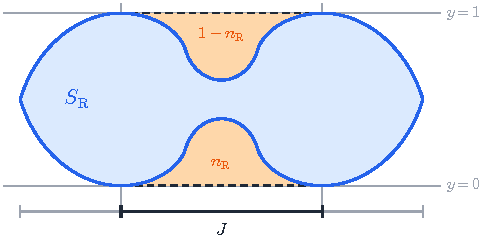
\includegraphics[width=.88\textwidth]{figures/fig-sofa.pdf}
 \caption{Romik's sofa is the hull (dashed) with the two open niches
 removed. Both niches lie over the middle half of the projection,
 and leave a positive band about $y=1/2$.}\label{fig:sofa}
\end{figure}

\begin{theorem}\label{thm:reference}
The set $\SR$ is an ambidextrous sofa of area $\Mc$ and
$\conv\SR=\HR$. It is invariant under reflection in $y=1/2$ and
is regular closed: $\clos(\inter\SR)=\SR$.
\end{theorem}
\begin{proof}
The set is closed in the compact hull. Every vertical fiber can be
joined within $\SR$ to the midline $y=1/2$, and the entire midline
segment over $I_{\KR}$ is present. This proves connectedness.
For the lower passage put $\phi=Lt$ and use the explicit placement
\begin{equation}\label{eq:reference-motion}
 p\longmapsto R_{-\phi}p+(1-F(\phi),1-G(\phi)),\qquad 0\le t\le1.
\end{equation}
The outer supporting half-planes give the two outer wall constraints.
The niche inequality gives the inner-corner alternative at every
interior angle. At $t=0$ the placement is the identity and the sofa
lies in $\Hin$; at $t=1$ it is
$(x,y)\mapsto(y,2-8A/3-x)$, which lies in $\Vm$ by the projection
and strip bounds. Reflection gives the upper passage with angle
$\phi$ and the same initial placement.

The boundary support points of $\HR$ survive the niche trimming.
The upper boundary arcs have abscissae outside the interior of the
top interval, where the niche is zero; their reflected arcs give
the remaining supports. Thus $\SR$ has the same
support function as $\HR$, which proves the convex-hull identity.
Finally the continuous strict niche band and the interior of the
hull approximate every boundary point from inside $\SR$. At points
on either niche boundary, a small displacement toward the midline
gives the approximation; the strict $1/2$ margin preserves the other
constraint. This proves regular closedness.

The area calculation follows below.
\end{proof}

\subsection{Exact value}
The value is obtained from the support functional $\mathcal A$
of \cref{sec:calibration}, before any optimality theorem is used.
For the reference pair, integration by parts in its Euler equations
evaluates the functional without integrating its algebraic boundary.
Put $p=F'-G+1$ and $q=G'+F-1$. On the first phase,
\[
 p=\tfrac12-2A\sin t,\qquad q=2A\cos t-1;
\]
on the middle phase, with $\varphi=t/2+\pi/8$,
\[
 p=1-\tfrac32R\sin\varphi,\qquad
 q=\tfrac32R\cos\varphi-1.
\]
The last phase is obtained by $p(L-t)=-q(t)$.
Thus $p\ge0$ on $[0,\beta]$ and $p\le0$ on $[\beta,L]$;
$q\ge0$ on $[0,L-\beta]$ and $q\le0$ afterwards.
At the switches $p(\beta)=q(L-\beta)=0$.

The Euler equations of \cref{eq:support-functional} on the three
phases are, respectively,
\[
 F''+F=0,\quad G''+G=\tfrac12;
\]
\[
 2F''-G'+F=0,\quad 2G''+F'+G=0;
\]
\[
 F''+F=\tfrac12,\quad G''+G=0.
\]
The displayed formulas for $F,G$ satisfy them by differentiation.
The two derivative fluxes are
\[
 J_F=-F'-(G-1)/2-p_-,\qquad
 J_G=-G'+(F-1)/2-q_+.
\]
They are continuous across both switches because the corresponding
contact momentum vanishes there. Their endpoint values are
\[
 J_F(0)=-\tfrac12,\quad J_G(0)=2-4A,
 \qquad J_F(L)=1,\quad J_G(L)=\tfrac12.
\]
Integration by parts therefore gives
\[
 D\mathcal A(F,G)[F,G]
   =[J_FF+J_GG]_0^L=\frac{16}3A-1.
\]
If $A_X$ denotes the functional density and $D_X$ its
self-variation density, expansion gives
\[
 2A_X-D_X=2-F-G+(F'-G')/2-p_-+q_+.
\]
Primitives of this remainder on the three phases are
\begin{align*}
 V_1(t)&=t/2+(2A-1/4)\cos t+(A-3/4)\sin t,\\
 V_2(t)&=(G(t)-F(t))/2,\\
 V_3(t)&=t/2-(1/4-A/3)\cos t-(3/4+2A/3)\sin t.
\end{align*}
Differentiating each primitive, with the corresponding contact
signs, verifies the remainder. Summing their increments and using
the matching values gives
\[
 2\mathcal A(F,G)-D\mathcal A(F,G)[F,G]
       =4A\cos\beta-\frac83A-1+\beta.
\]
Consequently
\begin{equation}\label{eq:reference-functional-value}
 \begin{aligned}
 \mathcal A(F,G)&=\frac43A+2A\cos\beta-1+\frac\beta2,\\
 P_L(\KR)&=\mathcal A(F,G)-\frac{w_{\KR}}2
          =2A\cos\beta-1+\frac\beta2.
 \end{aligned}
\end{equation}
For the second equality, \cref{lem:cap-support-area} expresses
the cap area by its support energy. The curvature bounds,
contact signs, and top face established above verify all the
hypotheses of \cref{cor:horizontal-score-identity}; its signed
graph calculation identifies the niche integral. This uses only
the reference geometry, independently of any optimality conclusion.

Since $4A\cos\beta=\cot\beta=1/Y$ and the cubic gives
$1/Y=4Y^2+3$, \cref{eq:reference-functional-value} yields
$P_L(\KR)=\Mc/2$. Cavalieri's principle now gives the body's area.
Outside $J_{\KR}$ the niche is zero; on $J_{\KR}$ the hull fills
the full unit-height fiber. Hence
\[
 \abs{\SR}
  =2\abs{\KR}-w_{\KR}-2\int_{J_{\KR}}\nR
  =2P_L(\KR)=\Mc.
\]


For comparison with Romik's closed form, put
$a=\sqrt[3]{\sqrt2+1}$ and $b=\sqrt[3]{\sqrt2-1}$, so $ab=1$.
Expansion shows that $Y=(a-b)/2$ solves the cubic and is positive.
Also
$1+4Y^2=a^2+b^2-1$. Therefore
\begin{equation}\label{eq:romik-radicals}
 \Mc=\sqrt[3]{3+2\sqrt2}+\sqrt[3]{3-2\sqrt2}-1
       +\arctan\!\left(\frac{\sqrt[3]{\sqrt2+1}
                            -\sqrt[3]{\sqrt2-1}}2\right).
\end{equation}

\section{Full-turn integral and contact estimates}\label{app:full-turn-estimates}

\subsection{Cap area and the signed niche integral}

Green's formula expresses both cap area and niche area through their
supports. The cap calculation follows the outer boundary. The niche
calculation joins a companion tangent, a reversed corner arc, and a
first tangent. Keeping these arcs oriented makes the formulas valid
even when a parametrized graph folds. Their difference will produce
the support functional of \cref{sec:calibration}.

For vectors $z,z'\in\R^2$, write $\det(z,z')$ for their determinant.
All oriented integrals below retain their sign when endpoints are
reversed.

\begin{lemma}[Cap support area]\label{lem:cap-support-area}
Let $U$ be a downward cap of height one, with quarter supports
$F(t)=h_U(t)$ and $G(t)=h_U(t+L)$. Suppose $F,G\in C^1[0,L]$
and their first derivatives are absolutely continuous. Then
\begin{equation}\label{eq:cap-support-area}
 2|U|=\int_0^L(F^2-F'^2+G^2-G'^2)\,\dd t.
\end{equation}
\end{lemma}
\begin{proof}
The upper boundary, oriented from right to left, has support
parametrization $z(\theta)=h(\theta)u(\theta)+h'(\theta)u^\perp(\theta)$.
On regular arcs
$\det(z,z')=h(h+h'')$ almost everywhere.
At the top normal $L$, the parametrization jumps along the top
segment. Its determinant integral is its horizontal length, because
its height is one. Put its endpoints at $x=x_{\rm tl},x_{\rm tr}$.
The one-sided support derivatives are
$h'(L-)=-x_{\rm tr}$ and $h'(L+)=-x_{\rm tl}$.
Integration by parts on the two quarter arcs therefore subtracts
exactly $x_{\rm tr}-x_{\rm tl}$, cancelling the top segment's
contribution.

At the right axis normal the derivative is the right end height
$e_R$; at the left normal it is $-e_L$. The remaining boundary
terms are $l_Ue_L-r_Ue_R$. The two vertical end faces contribute
$r_Ue_R-l_Ue_L$, and the baseline contributes zero.
Green's area formula now gives \cref{eq:cap-support-area}.
The absolutely continuous integration by parts is valid without
pointwise second derivatives. Approximation by polygonal boundary
arcs, or by smooth convex caps, justifies the same Green formula
when a curvature density vanishes on an interval.
\end{proof}
For two supports with top traces $F(L)=G(0)=1$, define
\[
 \begin{gathered}
 z=(F-1)u+(G-1)u^\perp,\\
 B=(F-1)u+F'u^\perp=z+pu^\perp,\\
 D=(G-1)u^\perp-G'u=z-qu.
 \end{gathered}
\]
Then
\begin{equation}\label{eq:corner-determinant}
 \det(z,z')=(F-1)^2+(G-1)^2+(F-1)G'-(G-1)F'.
\end{equation}

\begin{lemma}[Global contact from unit curvature]\label{lem:unit-global-contact}
Suppose the actual support densities satisfy $0\le F''+F\le1$
and $0\le G''+G\le1$ almost everywhere. At every interior angle $s$,
the following points lie on the graph of the complete positive niche:
\[
 B(s)\quad\text{if }p(s)\le0,\qquad
 D(s)\quad\text{if }q(s)\ge0,\qquad
 z(s)\quad\text{if }p(s)\le0\le q(s).
\]
\end{lemma}
\begin{proof}
The complementary profile $k=1-F$ has $k''+k\ge0$.
Variation of constants, or two integrations by parts, gives
\[
 k(t)-k(s)\cos(t-s)-k'(s)\sin(t-s)
 =\int_s^t(k''+k)(r)\sin(t-r)\,\dd r\ge0
\]
for $s,t\in[0,L]$, with the integral interpreted as oriented.
Thus $F(t)-1\le\ip{B(s)}{u(t)}$ for every $t$.
The analogous inequality is
$G(t)-1\le\ip{D(s)}{u^\perp(t)}$.
In particular $B_y,D_y\ge0$, by using $t=L$ and $t=0$.

At $B(s)$ the first-wall equality holds; the second-wall height is
at least $B_y$ precisely when $p(s)\le0$.
At all other angles the first-wall height is at most $B_y$.
Taking the supremum of the two-wall minima proves its niche contact.
The proof for $D(s)$ is the same.
For a corner $z(s)$ use the identities
\[
 \ip{z(s)}{u(t)}=\ip{B(s)}{u(t)}-p(s)\sin(t-s),
\]
\[
 \ip{z(s)}{u^\perp(t)}=\ip{D(s)}{u^\perp(t)}+q(s)\sin(s-t).
\]
For $t\ge s$ the first gives the required wall alternative, and
for $t\le s$ the second does. Both equalities hold at $s$.
Also $z_y=B_y-p\cos s\ge0$. These facts prove global contact
with the whole angular supremum, not only with neighboring angles.
\end{proof}

\begin{lemma}[Signed-roof integral]\label{lem:signed-roof}
Suppose $F,G\in C^1[0,L]$ have absolutely continuous first derivatives,
$F(L)=G(0)=1$, and $0\le b\le d\le L$ satisfy $p(b)=q(d)=0$.
Let $N$ be continuous, and suppose
\[
 \begin{aligned}
 N(D_x(t))&=D_y(t)&& (0<t<d),\\
 N(z_x(t))&=z_y(t)&& (b<t<d),\\
 N(B_x(t))&=B_y(t)&& (b<t<L).
 \end{aligned}
\]
Then
\begin{equation}\label{eq:signed-roof}
 2\int_{-G'(0)}^{-F'(L)}N(x)\,\dd x
 =-\int_0^L\det(z,z')\,\dd t
         +\int_b^L p^2\,\dd t+\int_0^d q^2\,\dd t.
\end{equation}
In particular, if $p\ge0$ before $b$, $p\le0$ after $b$,
$q\ge0$ before $d$, and $q\le0$ after $d$, the last two integrals
are $\int_0^L p_-^2$ and $\int_0^L q_+^2$.
\end{lemma}
\begin{proof}
For an absolutely continuous graph parametrization $Z=(X,Y)$ with
$Y=N(X)$, the chain rule applied to $\int^X N$ gives
$\int_X^{X'}N=\int YX'$. Also
\[
 2YX'=(XY)'-\det(Z,Z').
\]
This calculation needs no monotonicity of $X$.
Join the three oriented graph arcs $D:0\to d$, $z:d\to b$,
and $B:b\to L$. The joins agree because $p(b)=q(d)=0$.
Their outer endpoints have height zero and abscissae $-G'(0)$ and
$-F'(L)$. The $XY$ terms cancel, giving
\[
 2\int N=-\int_0^d\det(D,D')
                  +\int_b^d\det(z,z')-\int_b^L\det(B,B').
\]
Direct differentiation gives
\[
 \begin{aligned}
 \det(B,B')&=\det(z,z')-p^2+[(F-1)p]',\\
 \det(D,D')&=\det(z,z')-q^2+[(G-1)q]'.
 \end{aligned}
\]
Their endpoint terms vanish by the contact and top equations.
Combining the remaining corner integrals proves
\cref{eq:signed-roof}. The sign assumptions give the final assertion.
\end{proof}

\begin{corollary}[Actual horizontal score]\label{cor:horizontal-score-identity}
Suppose a height-one horizontal canonical cap has unit curvature
on both quarters, its top face is precisely $J_U$, and there are
ordered contact switches $b,d$ with the signs in
\cref{lem:signed-roof}. Then
\[
 P_L(U)=\mathcal A(F,G)-w_U/2.
\]
\end{corollary}
\begin{proof}
By \cref{lem:unit-global-contact}, all three graph identities hold
for $N=n_L(U)$. The top face gives
$-G'(0)=l_U+w_U/4$ and $-F'(L)=r_U-w_U/4$.
Subtract \cref{eq:signed-roof} from \cref{eq:cap-support-area}
and use \cref{eq:corner-determinant}. Since $f_U=1$ on $J_U$,
the score is $|U|-w_U/2-\int_{J_U}N$.
\end{proof}

\subsection{The three-tent estimate}

The diagonal hallway bounds the exterior roof and supplies one middle
tent. The two adjacent hallways add more niche area unless their
supports move inward; moving those supports inward cuts area from the
exterior roof. We combine these two payments by completing weighted
squares. The estimate uses only three visited angles and the endpoint
laws. Put
\[
 \begin{gathered}
 r=\sqrt2,\quad k=r-1,\quad c=\cos(\pi/8),\quad s=\sin(\pi/8),\\
 A=1-k,\quad b=2-k,\quad d=3r-1,\quad \gamma=1-r/2.
 \end{gathered}
\]
These letters are local to this subsection. In particular $c,s$ do
not refer to a terminal angle, and $A$ is not the reference parameter.
Useful identities are
\begin{equation}\label{eq:three-tent-constants}
 \frac sc=k,\quad k^2=1-2k,\quad \frac1s+\frac1c=4c,
 \quad \frac r{4c^2}=k,\quad 2d+b^2=9.
\end{equation}
Let a cap have projection $[-a,a]$, middle half $[-a/2,a/2]$,
and affine middle roof rising from $1-h$ to one. Lift the left wing
by $h$ and put the middle roof at one; retain the right wing.
Concavity is preserved, because the left slopes are at least $h/a$
and the right slopes are nonpositive. Denote the lifted cap by
$\widehat U$, and define
$u=rh_{\widehat U}(\pi/4)-1$ and
$v=rh_{\widehat U}(3\pi/4)-1$.
Then $a/2\le u,v\le a$. Put $m=(u+v)/2$ and define
\begin{align}\label{eq:three-tent-objective}
 F_h(a,u,v)&=a-\frac{(a-u)^2+(a-v)^2}{2}-\frac{ah}{2}
 -(m-h/2-k)^2\notag\\
 &\hspace{12mm}+\frac{(u-k-a/2)_+^2+(v-h-k-a/2)_+^2}{2},\\
 S(a,m,h)&=a/k+(k-2)m+3/2+2k-4c+h/4,\notag\\
 G_h(a,u,v)&=F_h(a,u,v)-S(a,m,h)_+^2/d.\notag
\end{align}

\begin{lemma}[Full three-tent score]\label{lem:full-three-tent-score}
Suppose $37/25\le a\le8/5$, $0\le h\le1/3$, and the actual
endpoint laws are
\[
 e_R=\tfrac12+\tfrac h4+(3n_+-n_-)/4,\qquad
 e_L=\tfrac12-\tfrac{3h}4+(3n_--n_+)/4,
\]
where $n_\pm=n_L(U)(\pm a/2)$.
With $t=2c-r$ and $d_0=3/5-t$,
\begin{equation}\label{eq:full-three-tent-score}
 P_L(U)\le G_h(a,u,v)+
 L(h),\qquad
 L(h)=\gamma[(d_0-h/4)^2+(d_0+3h/4)^2].
\end{equation}
\end{lemma}
\begin{proof}
The first diagonal support of $U$ is unchanged by lifting, because
$(a/2,1)$ dominates all lifted left-wing points. The second diagonal
parameter is $v-h$. Thus the actual diagonal niche is
$[\min(u-k-x,v-h-k+x)]_+$.
Its apex lies in the window and is positive. Its exact integral is
\[
 (m-h/2-k)^2
  -\tfrac12[(u-k-a/2)_+^2+(v-h-k-a/2)_+^2].
\]
The lifted roof lies below
$f_0(x)=\min(1,1+u-x,1+v+x)$.
Let $D$ be its exterior deficit from this roof. Integrating $f_0$
and undoing the left lift gives
$P_L(U)\le F_h-D-(\int_J n_L-\int_Jn_{45})$.

The box-wall bound gives $n_\pm\le1-\sqrt{1-(a/2)^2}\le2/5$.
The endpoint laws then imply
\[
 e_R\ge2/5+h/4,\quad e_L\ge2/5-3h/4,
 \quad e_R+e_L\ge1-h/2.
\]
Writing $w_R=a-u$ and $w_L=a-v+h$, support containment gives
\[
 e_R\le1-w_R,\quad e_L\le1-w_L,
 \quad w_R\le3/5-h/4,\quad w_L\le3/5+3h/4.
\]
Let
$\delta_L=c+sv-h_{\widehat U}(5\pi/8)$ and
$\delta_R=c+su-h_{\widehat U}(3\pi/8)$.
Both are nonnegative. On the two flat pieces of $f_0$, the near
vertical supporting lines cut disjoint triangles of total area
$D_0=r(\delta_L^2+\delta_R^2)\le D$.
They fit before the middle window since
$\delta_L\le s(v-a/2)$ and $\delta_R\le s(u-a/2)$.

The niche at $\pi/8$ dominates the tent
\[
 \begin{gathered}
 f_R(x)=\min(b_R+kx,B_R-x/k),\\
 b_R=1-1/c+kv-h-\delta_L/c,\qquad B_R=e_R+a/k-1/s.
 \end{gathered}
\]
Against the descending diagonal branch its signed peak is
$Z_R=(B_R+b_R)/2-u+k$, with crossover endpoints
\[
 x_L=(u-k-b_R)/r,\qquad x_R=(B_R-u+k)/r.
\]
The reflected construction at $3\pi/8$ gives
\[
 \begin{gathered}
 b_L=1-1/c+ku-\delta_R/c,\quad B_L=e_L+a/k-1/s,\\
 Z_L=(B_L+b_L)/2-v+h+k.
 \end{gathered}
\]
The two triangles lie on opposite sides of the diagonal apex:
their crossover displacements from it are
$k(m\pm h/2)+2s-1+\delta/(rc)>0$.
Indeed $m-h/2\ge3/4$, $k>2/5$, and $2s>3/4$.
Their outer endpoints satisfy
$x_R\le1+a-2c<a/2$, since $a/2\le4/5$ and $c>9/10$;
the reflected endpoint satisfies the same inequality.
Thus both complete signed gain triangles fit inside $J$ whenever
their peaks are positive.

For a signed triangle of height $Z>0$ and slopes $r,-r$, whose
baseline zero exceeds its right endpoint by $\Delta$, the positive
floor loses at most $\gamma\Delta_+^2$ from the signed area
$Z^2/r$. To check this, use the coordinate $q=x_R-x$.
If $0<\Delta\le rZ$, the loss is
\[
 \int_0^{k\Delta}rq\,\dd q+
 \int_{k\Delta}^{\Delta}(\Delta-q)\,\dd q
   =\tfrac12[rk^2+(1-k)^2]\Delta^2=\gamma\Delta^2.
\]
If $\Delta>rZ$, the remaining positive tent has area
$r[(1+1/r)Z-\Delta]_+^2$.
When its bracket is nonnegative, subtracting
$Z^2/r-\gamma\Delta^2$ leaves
$(1+r/2)(\Delta-rZ)^2\ge0$.
When the bracket is negative the latter bound is already
nonpositive. The case $Z\le0$ needs no positive interval.
For the two triangles the losses satisfy
$\Delta_R\le(w_R-t)_+$ and $\Delta_L\le(w_L-t)_+$,
so their total is at most $L(h)$.

Write $Z_R=Z_R^0-\delta_L/(2c)$ and
$Z_L=Z_L^0-\delta_R/(2c)$.
The endpoint-height sum gives $Z_R^0+Z_L^0\ge S(a,m,h)$.
If $H_0=((Z_R)_+^2+(Z_L)_+^2)/r$, Cauchy--Schwarz gives
\[
 S_+\le\sqrt{2rH_0}+\sqrt{rD_0/(4c^2)},\qquad
 S_+^2\le(2r+r/(4c^2))(H_0+D_0)=d(H_0+D_0).
\]
Combining the exterior deficit, diagonal niche, additional two
triangles, and floor correction proves
\cref{eq:full-three-tent-score}. Each exterior deficit is charged
once, and the two niche gain regions are disjoint.
\end{proof}

\begin{lemma}[Stationarity and the width derivative]\label{lem:three-tent-general-plane}
Fix $h\ge0$ and a comparison width $a_0$. Put
\[
 \sigma=s_0(a_0)-Ah/4,\quad
 s_0(a)=da/2-(4c-2),\quad
 m_*=(a_0+k)/2+b\sigma/9+h/4.
\]
Suppose
\[
 \sigma\ge0,\qquad m_*\le k+a_0/2,\qquad
 r-a_0-2d\sigma/9\le0.
\]
Then for $a\ge a_0$ and diagonal data with nonnegative apex,
\[
 G_h(a,u,v)\le
 B(a_0)-kh/2-h^2/8-2\sigma^2/9,
 \qquad B(a)=a-(a-k)^2/2.
\]
\end{lemma}
\begin{proof}
Use coordinates $(a,m,\Delta)$, with $\Delta=(u-v)/2$.
Before the two clipping terms the Hessian of $F_h$ is
\[
 \begin{pmatrix}-2&2&0\\2&-4&0\\0&0&-2\end{pmatrix}.
\]
Each active clip adds the outer product of $(-1/2,1,1)$ or
$(-1/2,1,-1)$. With both present the Hessian is
\[
 \begin{pmatrix}-3/2&1&0\\1&-2&0\\0&0&0\end{pmatrix},
\]
which is negative semidefinite. Any other clipping pattern subtracts
a positive semidefinite matrix. The gradients match at the interfaces,
and subtracting $S_+^2/d$ preserves joint concavity.

At $u=v=m$ in the unclipped region put $m'=m-h/4$ and
$m_0(a)=(a+k)/2$. Completion of squares gives
\[
 G_h=B(a)-kh/2-h^2/8-2(m'-m_0(a))^2
       -[s_0(a)-b(m'-m_0(a))-Ah/4]^2/d.
\]
Since $2d+b^2=9$, both support derivatives vanish at
$(a,u,v)=(a_0,m_*,m_*)$. The clipping hypothesis makes the
right clip zero; the left clip is smaller by $h$. Also
$S=2d\sigma/9\ge0$. The value there is the asserted bound,
and its width derivative is $r-a_0-2d\sigma/9$.
The tangent plane of a concave function is an upper bound everywhere.
Its support derivatives vanish and its width derivative is nonpositive,
so it bounds every larger width by this value.
\end{proof}

\begin{lemma}[Three-tent supporting plane]\label{lem:full-three-tent-critical}
Fix $0\le h\le1/3$ and put
\[
 \begin{gathered}
 a_0=37/25,\qquad B(a)=a-(a-k)^2/2,\\
 s_0(a)=da/2-(4c-2),\qquad m_0(a)=(a+k)/2.
 \end{gathered}
\]
On $a\ge a_0$, $a/2\le u,v\le a$, the function $G_h$ is
jointly concave and
\begin{equation}\label{eq:three-tent-supporting-plane}
 G_h(a,u,v)\le
 K_0(h):=B(a_0)-kh/2-h^2/8
             -\tfrac29[s_0(a_0)-Ah/4]^2.
\end{equation}
\end{lemma}
\begin{proof}
Apply \cref{lem:three-tent-general-plane}. At $a_0=37/25$ its
stationary support coordinate is
\[
 u_*=v_*=(a_0+k)/2+\frac b9[s_0(a_0)-Ah/4]+h/4.
\]
To check clipping, keep the angle parameters linked by
$k^2+2k=1$ and $2c^2(1-k)=1$. With
$\mathcal N_q(x)=(x+q/x)/2$, define
\begin{equation}\label{eq:triangle-newton-parameters}
 \begin{gathered}
 k_+=\mathcal N_2(\mathcal N_2(3/2))-1,
 \qquad k_-=2/(1+k_+)-1,\\
 Q_\pm=2-2k_\pm,\qquad
 c_-=[\mathcal N_{Q_-}(\mathcal N_{Q_-}(1))]^{-1},\qquad
 c_+=\mathcal N_{Q_+}(\mathcal N_{Q_+}(1))/Q_+.
 \end{gathered}
\end{equation}
Squaring the Newton inequality gives $k_-<k<k_+$ and
$c_-<c<c_+$. Write
$s_+=(2+3k_+)a_0/2-(4c_--2)$.
Substitution in these formulas gives $2/3<s_0(a_0)<s_+<3/4$
and $s_0(a_0)-Ah/4>0$. Since $bA=3-5k$, the larger clip obeys
\[
 u_*-k-a_0/2
 <-k_-/2+(2-k_-)s_+/9+(6+5k_+)(1/3)/36<0.
\]
The last inequality follows by inserting the Newton formulas;
no separately chosen bound on the support coordinate is needed.
The other clip is smaller by $h$.
Also $a_0/2<u_*<a_0$, and $S>0$ there.
The width derivative is negative because
\[
 r-a_0-\frac{2d}{9}[s_0(a_0)-Ah/4]<r-a_0<0.
\]
These checks verify the hypotheses of
\cref{lem:three-tent-general-plane}, which gives the bound $K_0(h)$
for all $a\ge a_0$.
\end{proof}

The floor corrections in the full, proper, and dry-endpoint comparisons
have the same form. The following payment separates the geometric loss
from the final arithmetic check.

\begin{lemma}[Tilt pays for the floor]\label{lem:triangle-tilt-payment}
Let $\sigma=s_0(a_0)$ and put
\[
 \Psi(h)=B(a_0)-kh/2-h^2/8-\tfrac29(\sigma-Ah/4)^2
       +\gamma[(p+\lambda h)^2+(q+\mu h)^2].
\]
If $k\ge2/5$, $k\le1$, $\sigma\le3/4$,
$\lambda p+\mu q\le1/6$, $\lambda^2+\mu^2\le5/8$, and
$0\le h_0\le h$ with $h+h_0\le1/2$, then $\Psi(h)\le\Psi(h_0)$.
\end{lemma}
\begin{proof}
Subtract at $h_0$ and factor out $h-h_0$. The remaining factor is
\[
 -k/2+A\sigma/9+A(\lambda p+\mu q)
 +(h+h_0)[-1/8-A^2/72+A(\lambda^2+\mu^2)/2].
\]
Since $0\le A\le3/5$, it is at most
\[
 -1/5+1/20+1/10+1/32<0.
\]
The first term is the direct tilt cost; the next two pay for
moving the stationary point and the floor cuts. The last pays
for their quadratic remainder.
\end{proof}

For the three applications, $t=2c-(1+k)$ and the data are
\[
\begin{array}{c|cccc|c}
 &p&q&\lambda&\mu&h_0\\ \hline
 \text{full}&3/5-t&3/5-t&-1/4&3/4&0\\
 \text{proper}&0&2/3-t&0&2/3&0\\
 \text{dry endpoint}&1/2-t&7/12-t&-1/4&3/4&0
\end{array}
\]
The Newton enclosures give $5/12<t<1/2$.
Thus $\lambda p+\mu q\le1/6$ in every row, and the largest
$\lambda^2+\mu^2$ is $5/8$, from the endpoint-law slopes
$-1/4,3/4$. The allowed heights satisfy $h+h_0<1/2$.
One tilt payment therefore covers all three exclusions.

\paragraph{The width fixed by the initial radius}

A dry low endpoint makes the initial momentum
$B=b(h)+3n_+/4$, where $b(h)=-1/2+5h/4$.
The radius test allows span $R(h)=\sqrt{5-b(h)^2}$.
The box gives $n_+\le1/3$, so the largest momentum at height $h$
is $b(h)+1/4$. Choose the height where its floor-energy test meets
four at that allowed radius:
\begin{equation}\label{eq:tilted-balance-height}
 R(h_0)^2+[b(h_0)+1/4]^2+[b(h_0)+1/4](1-h_0)
 -R(h_0)\sqrt{h_0(2-h_0)}=4.
\end{equation}
This determines a unique $h_0\in(0,1/3)$.
To check existence and obtain bounds, put
\[
 \begin{aligned}
 V(h)&=R(h)^2+[b(h)+1/4]^2+[b(h)+1/4](1-h)-4,\\
 F(h)&=V(h)^2-R(h)^2h(2-h).
 \end{aligned}
\]
Here $V$ is positive; $F$ decreases on $[0,1/3]$ and changes sign
between its endpoints. The squared equation therefore gives the
same height. Starting with $[l,u]=[0,1/3]$, three simultaneous updates
\[
 (l,u)\longmapsto\left(l-\frac{F(l)}{F'(l)},\,
                        u-\frac{F(u)}{F'(l)}\right)
\]
give bounds $h_-\le h_0\le h_+$.
The divided difference of $F$ lies above $F'(l)$ on each bracket,
so these are enclosing updates, rather than fitted approximations.
The shared radius width is now
\begin{equation}\label{eq:tilted-radius-width}
\begin{gathered}
b_0=b(h_0),\quad R_0=R(h_0),\quad C_{\rm rad}=R_0/3,\\
R_+=\mathcal N_{R(h_+)^2}^{\circ2}(2),\qquad
R_-=R(h_-)^2/R_+,\qquad a_{\rm rad}=2R_-/3.
\end{gathered}
\end{equation}
The span lower bound $d\ge2$ supplies the Newton seed.
The brackets give $R_-<R_0<R_+$.
The triangle comparison below excludes every larger width, even when
$h<h_0$, and can be evaluated at zero tilt like the other two rows.
Both boundaries are therefore fixed by the two energy tests.

\begin{lemma}[A common endpoint comparison]\label{lem:triangle-newton-corners}
Use $k_+,c_+$ from \eqref{eq:triangle-newton-parameters} and define
\[
\begin{aligned}
 E&=(a+1-h/2)k+a-(a^2+1)/2-h^2/8\\
  &\quad-2z^2/9+\tfrac A2(wD_R^2+D_L^2),\\
 z&=(2+3k)a/2-(4c-2)-Ah/4,\\
 D_i&=b_i-(2c-1-k).
\end{aligned}
\]
For each of the following geometric endpoint data,
$E(a,h,k,c;b_R,b_L,w)\le E(a,h,k_+,c_+;b_R,b_L,w)<\underline p$:
\[
\begin{array}{c|ccccc}
 &a&h&b_R&b_L&w\\ \hline
 \text{full}&37/25&0&3/5&3/5&1\\
 \text{proper}&37/25&0&2/3&2/3&0\\
 \text{dry endpoint}&a_{\rm rad}&0&1/2&7/12&1
\end{array}
\]
Here $w=0$ records the proper comparison's single joint floor square.
\end{lemma}
\begin{proof}
The identity $k^2+2k=1$ rewrites $B(a)$ as the linear term in
$E$. To bound the whole expression, first increase $c$ to $c_+$,
then increase $k$ to $k_+$. On these segments, the Newton enclosures
give $3/5\le z\le3/4$ and $0\le D_i\le1/4$.
The two changes both raise $E$:
\[
 \partial_cE=16z/9-2A(wD_R+D_L)>0,
\]
\[
\begin{aligned}
 \partial_kE&=a+1-h/2-\tfrac49(3a/2+h/4)z\\
 &\quad-\tfrac12(wD_R^2+D_L^2)+A(wD_R+D_L)\\
 &\ge a/2+15/16-7h/12>0.
\end{aligned}
\]
Here $0\le w\le1$, and all three rows have $h=0$.
The first comparison retains the improvement in the stationary square
alongside the loss in floor payment; the second retains the linear
area reward. Both can equally be obtained by subtracting the two
squares. Inserting the same Newton formulas in each row gives
$E<\underline p$ using \eqref{eq:reference-half-area-lower}.
\end{proof}

\begin{corollary}[Full width cut]\label{cor:full-three-tent-cut}
Every cap satisfying the hypotheses of
\cref{lem:full-three-tent-score} has $P_L(U)<\underline p$.
\end{corollary}
\begin{proof}
By \cref{lem:full-three-tent-critical},
$P_L(U)\le K_0(h)+L(h)$.
The full row of \cref{lem:triangle-tilt-payment} bounds this at $h=0$.
Its value is the full row of \cref{lem:triangle-newton-corners},
which is below $\underline p$.
\end{proof}

\subsection{The first-wing energy test}
\label{app:first-wing-energy}

The following estimates use the tilted notation of
\cref{sec:full-turn}. In particular $I=[-2C,2C]$, $J=[-C,C]$,
the middle roof rises from $1-h$ to $1$, and $F,G$ are the
high-wing and low-wing supports. Write
\[
 d=3C,\qquad B=e_R-1+h,\qquad
 s_h=\sqrt{h(2-h)},\qquad H(C)=1-\sqrt{1-C^2}.
\]

The target $u\le1$ follows if $q\le1$ whenever the first source can
be exposed. At its first $p$-zero this means $q+1\le2$. Before the
corner reaches the floor, the support trajectory is a free rotation.
The two tests below bound its energy depending on which event comes
first; the constants four and five are the corresponding squared
radii.

\begin{lemma}[Initial-floor test]\label{lem:tilted-initial-energy}
Suppose $1/2<C<4/5$ and $0<h<1/3$. At a canonical full
maximum, the two inequalities
\begin{equation}\label{eq:tilted-initial-energy}
 d^2+B^2\le5,\qquad
 d^2+B^2+B(1-h)-d s_h\le4
\end{equation}
imply $u\le1$ almost everywhere on $(0,L)$.
\end{lemma}
\begin{proof}
On the initial component where $p,q>0$ and $D_y<0$, both source
densities vanish. The first vanishes by same-sign shadowing.
A positive second-source contact with companion slack would have
to be the stationary second-wall contact $D$, whose height is
negative. A corner is shadowed because both its walls increase
with the angle. The source identity therefore makes the second
density zero as well. This reasoning also excludes a floor
contact: a nonstationary one with slack is raised by a nearby
angle, and a same-sign floor corner is raised on both walls.
Compact exhaustion in angle justifies the statement at the
level of the limiting source measures.

Consequently, until this component meets the floor or $p=0$,
\begin{equation}\label{eq:initial-floor-solution}
 \begin{gathered}
 F=2C\cos t+e_R\sin t,\qquad
 G=C\sin t+(1-h)\cos t,\\
 D_y=1-h-\cos t,\\
 p-1=B\cos t-d\sin t,\qquad
 q+1=d\cos t+B\sin t.
 \end{gathered}
\end{equation}
Put $\gamma_0=\arccos(1-h)$ and let $\alpha$ be the first
$p$-zero on the initial positive-$q$ component. Stop at
$\min(\alpha,\gamma_0)$. The rotating vector in
\cref{eq:initial-floor-solution} has squared norm $R^2=d^2+B^2$.
Thus
\[
 \begin{aligned}
 E_{++}:=(p-1/2)^2+(q+1)^2&=R^2+p-3/4\\
 &\le R^2+1/4+\max\{B(1-h)-ds_h,-1\}
 \end{aligned}
\]
at the stopping time. The $-1$ alternative is the value when
$p=0$; the other alternative is the value at the floor.
Both tests in \cref{eq:tilted-initial-energy} say that this upper
bound is at most $17/4$.

If the floor is reached first, the same-sign bounds $u=0$,
$v\le1/2$ give
\[
 E_{++}'=2(p-1/2)(-1-q)+2(q+1)(v-1+p)
        =2(q+1)(v-1/2)\le0.
\]
At the first $p$-zero, $1/4+(q+1)^2\le17/4$, hence $q\le1$.
While $p<0$ and $q>0$, the arm estimate gives $q'\le-1/2$:
for $-1\le p\le0$ use $v\le(1-p)/2$, and for $p<-1$
use $v\le-p$. The positive-$q$ component therefore has $q\le1$
after this zero.

Any later positive-$q$ component starts at $q=0$ with $0<p\le1$;
entry with $p\le0$ is excluded by the preceding derivative bound.
While $p,q>0$, $u=0$, $p'\le-1$ and $q'\le p-1/2$.
Its maximum $q$ is at most
$\int_{1/2}^1(x-1/2)\,\dd x=1/8$. Once $p$ is negative,
$q$ decreases again. If the initial positive-$q$ component ends
before the stopping time, only these later components need be
considered. Finally $q\ge-1$ everywhere, and
$u\le\kappa(q)$, with $u=0$ in the positive-positive sector.
The proved bounds $-1\le q\le1$ on all remaining sectors give
$u\le1$.
\end{proof}

\begin{lemma}[Short widths and the radius width]\label{lem:tilted-unit-regions}
The first density of a canonical full maximum is at most one if
\(C\le2/3\). If its low middle endpoint is dry, the same conclusion
holds for \(C\le C_{\rm rad}\) and \(h_0\le h<1/3\), with
\(C_{\rm rad},h_0\) from \eqref{eq:tilted-radius-width}.
\end{lemma}
\begin{proof}
For \(C\le2/3\), write \(e=e_R\in[0,1]\).
Then \(d^2\le4\), \(|B|=|e-1+h|\le1\) and \(s_h\ge h\).
The first test follows at once. The second follows from
\[
B^2+B(1-h)=e(e-1+h),\qquad
 e(e-1+h)-ds_h\le h(e-d)\le0,
\]
since \(d>3/2\ge e\).

Now assume \(2/3<C\le C_{\rm rad}\), \(h\ge h_0\), and \(n_-=0\).
Since \(9C_{\rm rad}^2=5-b_0^2<5\), the box height obeys
\(H(C)\le1/3\). The dry endpoint pressure therefore gives
\[
-1/2+5h/4\le B\le-1/4+5h/4.
\]
On \([h_0,1/3]\) both endpoints have absolute value at most
\(-b_0\), and hence
\[
d^2+B^2\le9C_{\rm rad}^2+b_0^2=5.
\]
This is exactly why the radius width was chosen.

For the floor test put
\(Q(d,B,h)=d^2+B^2+B(1-h)-d\sqrt{h(2-h)}\).
It increases with \(B\) on this interval, since
\(2B+1-h\ge3h/2\ge0\), and with \(d\ge2\).
Thus it suffices to use $d=R_0$ and $B=-1/4+5h/4$.
The resulting function is convex in $h$: its polynomial part
has quadratic coefficient $5/16$, and the negative semicircle is convex.
Only the two endpoints $h=h_0,1/3$ remain.
At $h_0$ the test equals four by its defining equation.
At $1/3$, use $R_0^2\le5$, $R_0\ge2$ and
$\sqrt{(1/3)(2-1/3)}\ge2/3$. These give
\[
 Q(R_0,1/6,1/3)\le5+(1/6)^2+(1/6)(2/3)-2(2/3)<4.
\]
Convexity supplies the whole interval.
Apply \cref{lem:tilted-initial-energy}.
\end{proof}

\subsection{Ordered contact geometry}

Here $F,G,u,v,p,q,z,B,D,C,h,T$ have the tilted meanings in
\cref{eq:tilted-wing-supports,eq:tilted-contact-data}. In
particular $G(0)=1-h$; it is the low-wing support, not the
support containing the middle facet.

\begin{lemma}[Contact signs]\label{lem:tilted-contact-signs}
If $1/2<C<4/5$, $0<h<1/2$ and $u\le1$ almost everywhere,
there are $0<\alpha<\eta<L$ such that
\[
 \begin{array}{c|ccc}
 t&(0,\alpha)&(\alpha,\eta)&(\eta,L)\\ \hline
 p&>0&<0&<0\\
 q&>0&>0&<0.
 \end{array}
\]
Moreover $p(\alpha)=q(\eta)=0$.
\end{lemma}
\begin{proof}
Initially $p(0)=e_R+h>0$, $q(0)=3C-1>0$, whereas
$p(L)=1-3C-T<0$ and $q(L)=-e_L<0$.
Before $\delta=\arctan(h/(2C))$, the zero-density solution
gives $q'\ge-1$ while $p$ is positive. Since
$\delta<h<1/2<q(0)$, $q$ cannot reach zero there.
After $\delta$, the arm bound gives $p\le1$.
On the positive-positive sector, $u=0$, and
\[
 [(p-1)^2+(q+1)^2]'=2(q+1)v\ge0.
\]
Its initial value is at least $9C^2>2$. A first exit through
$q=0$ would instead have $0\le p\le1$ and energy at most two.
Thus the first exit is $p=0$, at a time $\alpha$, with $q>0$.

For $q\ge0$, the arm bound gives
$p'=u-1-q\le\kappa(q)-1-q\le-1/2$.
For $p\le0$, the companion bound similarly gives $q'\le-1/2$.
Consequently $p$ stays negative while $q>0$, and $q$ reaches
zero at some $\eta>\alpha$ with $p(\eta)<0$.
In the ensuing negative-negative sector $v=0$, $u\le1/2$ and
\[
 [(p-1)^2+(q+1/2)^2]'=2(p-1)(u-1/2)\ge0.
\]
At $\eta$ this energy is strictly greater than $5/4$.
A return through $p=0$ would have $-1\le q\le0$ and energy
at most $5/4$, since the lower arm bound is $q\ge-1$.
Such a return is impossible. As long as $p<0$, the preceding
$q'\le-1/2$ bound also prohibits a return through $q=0$.
This proves all the signs, including strictness at the ends of
the open sectors. The argument uses first crossing times of
continuous functions and integrated almost-everywhere derivative
bounds, so it covers zero-density intervals.
\end{proof}

\begin{lemma}[First-unit contact geometry]
\label{lem:tilted-first-unit-geometry}
Under the hypotheses of \cref{lem:tilted-contact-signs},
$B_x$ is nondecreasing and $B_y$ is nonincreasing. Let $\beta$
be its first crossing of $C$ (use $\beta=L$ when $T=0$).
Then
\begin{equation}\label{eq:tilted-crossing-box}
 \alpha<\beta,\qquad \beta\ge\arccos C,\qquad
 \sin\beta\ge3/5,\qquad \cot\beta\le4/3.
\end{equation}
The positive niche is precisely $(x_*,C+T)$ for one
$x_*<1-2C$, and
\begin{equation}\label{eq:tilted-no-ghost-projection}
 T=(C+x_*)_+.
\end{equation}
If the companion density exceeds one, its first bad entry
$\tau$ satisfies
\begin{equation}\label{eq:tilted-first-bad-bound}
 \alpha<\beta<\tau<\eta,\quad
 p(\tau)=-1,\quad 0<q(\tau)\le1/4,
 \qquad v\le1\text{ a.e. on }(0,\tau).
\end{equation}
In particular $T=0$ implies $v\le1$ almost everywhere.
\end{lemma}
\begin{proof}
The monotonicity follows from $B'=(u-1)u^\perp$ and $u\le1$.
If $B_x\ge C$, its associated outer point
$(X,Y)=B+u(t)$ lies in the cap, so $\cos t\le C$ and
$X\ge C+\cos t$, $Y\le1$. The low endpoint gives
$G\ge C\sin t+(1-h)\cos t$, whence
\[
 p\le1-(2C+\cos t)\sin t+h\cos t<0.
\]
For the last sign put $k=\cos t\in[0,C]$. The upper bound
$1-(2C+k)\sqrt{1-k^2}+k/2$ is convex in $k$.
At zero it is $1-2C<0$; at $C$ it is negative because
\[
 9C^2(1-C^2)-(1+C/2)^2>0\quad(1/2\le C\le4/5).
\]
This polynomial has derivative
$(2-3C)(24C^2+16C-1)/2$, hence its minimum is at an
endpoint; its endpoint values are $1/8$ and $71/625$.
Thus $B_x(\alpha)<C$, proving the first inequality in
\cref{eq:tilted-crossing-box}; the outer point at the crossing
gives the remaining three.

For the positive set write
\[
 \begin{gathered}
 R_t(x)=\frac{F(t)-1-x\cos t}{\sin t},\qquad
 S_t(x)=\frac{G(t)-1+x\sin t}{\cos t},\\
 L_0(t)=\frac{1-G(t)}{\sin t}.
 \end{gathered}
\]
On $x<1-2C$, the envelope $\sup_t S_t(x)$ is finite, convex,
and nondecreasing in $x$. Its endpoint limits are $-h$ at
zero and $-\infty$ at $L$. It is at most $-h$ for
$x\le-2C$, by the low-wing box $[-2C,-C]\times[0,1-h]$;
at $x=1-2C$ its $L$-limit is $e_L>0$.
There is exactly one zero $x_*\in(-2C,1-2C)$.
Indeed a zero is attained at an interior angle and that wall
has positive slope $\tan t$, so all points to its right have
positive envelope. All points to its left have negative envelope.
Equivalently $x_*=\inf_t L_0(t)$.

The derivative of $(F-1)/\cos t$ is $B_y/\cos^2t\ge0$.
Its intercept therefore rises from $2C-1$ to $C+T$.
Every first wall is positive for $x\le1-2C<2C-1$, and
every first wall is nonpositive for $x\ge C+T$.
For $1-2C<x<C+T$, angles approaching $L$ give
$R_t(x)=(C+T-x)(L-t)+o(L-t)>0$ and $S_t(x)\to+\infty$.
This proves the positive interval. The additional actual
high-point wall is nonpositive on $J$ and does not affect it there.

The finite positive graph has horizontal length equal to the
sine/cosine moment of its two source measures. Source convergence
and \cref{eq:tilted-wing-traces} give its limiting length as
\[
 \int_0^L(u\sin t+v\cos t)\,\dd t=2C-T.
\]
Uniform niche convergence gives the lower bound from the positive
interval. To get the reverse bound, take a compact interval
strictly left of $x_*$. All surrogate second walls there are strictly
negative when their angles lie in $[\varepsilon,L-\varepsilon]$.
The additional actual high-point wall is also strictly negative
there. The finite positive graph on this compact interval must
therefore use endpoint-angle sources. Their total mass is
$O(\varepsilon)+o(1)$ by \cref{eq:variation-coarse}.
Exhaust the zero interval and then let $\varepsilon\downarrow0$.
Thus the finite positive lengths converge to
$C-\max\{-C,x_*\}$. Equating the two lengths proves
\cref{eq:tilted-no-ghost-projection}.

Let $\tau$ be the first entry into $\{p<-1,q>0\}$.
Before it, $v\le1$: use $v\le\kappa(p)$ when $p\ge-1$,
and $v=0$ in the negative-negative sector when $p<-1$.
On a level set $q=0$, its derivative is zero almost everywhere,
whereas $p<-1$ would give $q'\le-1$; no exceptional mass remains.
Entry through $q=0$ is impossible because $q'\le-1/2$ for
$p\le0$. Thus $p(\tau)=-1$, $q(\tau)>0$.

For $\alpha<t<\tau$, past $D_x$ is nondecreasing, whereas
future $B_x$ is globally nondecreasing. Hence the positive core
corner is the unique active angle: earlier second walls and
later first walls are strictly below it. It lies in $J$, since
$-C<D_x+q\cos t=z_x=B_x+p\sin t<C$.
It contributes first-source density $q$. Before $\beta$,
the disjoint visible $B$ tangency contributes another $1-u$.
The source identity gives
$u\ge(1+q)/2$ before $\beta$, and $u\ge q$ after it.
Plateaus contribute zero tangent length and do not change these
bounds. If $\tau\le\beta$, the bounds $u\le1$ and
$u\le\kappa(q)$ make $q\le1$, $u=(1+q)/2$ on the core
up to $\tau$. There
$E=(p-1)^2+(q+1)^2$ is nonincreasing and $E(\alpha)\le5$;
but $E(\tau)=4+(q(\tau)+1)^2>5$, a contradiction.
The same strict comparison at the crossing excludes equality
$\tau=\beta$.

On $(\beta,\tau)$, put $K=q+(p-1)^2/4$.
Since $u\ge q$ and $-1<p<0$, $v\le(1-p)/2$ gives
$K'\le v+(p-1)/2\le0$.
At $\beta$, $E\le5$ yields
\[
 K(\beta)\le1+q(\beta)/2-q(\beta)^2/4\le5/4.
\]
As $K(\tau)=1+q(\tau)$, this proves
\cref{eq:tilted-first-bad-bound}. If $T=0$, $\beta=L$ and
the first bad entry is impossible; the arm and same-sign
bounds then give $v\le1$ everywhere.
\end{proof}

\subsection{The joint occupation of a corner}

A visible corner belongs to both wall families. Resolving its tangent
vector into those two wall directions fixes the ratio of their source
lengths. Thus both families must use the same occupied fraction of a
corner. This shared fraction is what lets the energy argument pay for
folds without counting a contact twice.

\begin{lemma}[Common source occupation]
\label{lem:variation-joint-occupation}
Under the first-unit hypotheses, suppose the companion density
exceeds one on a set of positive measure, and let the
ordered contacts and $\beta$ be as above. There are measurable
$d,\chi\in[0,1]$ such that, almost everywhere,
\begin{equation}\label{eq:joint-source-equations}
 \begin{array}{c|cc}
 &u&v\\ \hline
 (0,\alpha)&0&(1-v)d\\
 (\alpha,\eta)&(1-u)b+q\chi&(1-v)d-p\chi\\
 (\eta,L)&0&0,
 \end{array}
 \qquad b=\mathbf1_{\{t<\beta\}}.
\end{equation}
The second tangent occupation satisfies $d=0$ where $v>1$ or
$D_y<0$. Before a first bad entry $\tau$, one has $\chi=1$
on $(\alpha,\tau)$.
\end{lemma}
\begin{proof}
Keep the source angle and graph abscissa together in the finite
polygons. Assign to every positive first-source segment its
arclength measure at $(t,x)$; call this $\mu_{i,F}$, and
define $\mu_{i,G}$ similarly. Their exact graph-vector identities
on the window interior are
\begin{align*}
 \pi_{x\#}(\sin t\,\mu_{i,F}+\cos t\,\mu_{i,G})
   &=\mathbf1_{\{N_i>0\}\cap J_i}\,\dd x,\\
 \pi_{x\#}(-\cos t\,\mu_{i,F}+\sin t\,\mu_{i,G})
   &=\dd(N_i|_{J_i}).
\end{align*}
The second is a distributional identity. Bounded mass gives a
joint weak subsequence. The no-ghost argument in
\cref{lem:tilted-first-unit-geometry} passes the first identity
to Lebesgue measure on $(x_*,C)$. Uniform graph convergence
passes the second to $N'(x)\,\dd x$ on this positive interval.
The angular marginals are exactly $u\,\dd t,v\,\dd t$ by
\cref{lem:variation-sources}. There are no endpoint-angle atoms.
The graph is locally Lipschitz on its positive interval:
on a compact positive part, the endpoint-angle walls tend to
zero or below, so all active angles remain in a compact
subinterval of $(0,L)$. These identities also exclude extra
mass at a spatial singleton or at a floor point.

At a regular positive active source with first-wall slack,
angular stationarity gives $x=B_x(t)$ and height $B_y(t)$;
this needs $p<0$. The analogous second-wall contact is $D$,
with $q>0$. A simultaneous contact is $z$.
A corner with two positive momenta is shadowed by a slightly
larger angle, and one with two negative momenta by a slightly
smaller angle. Thus only core corners remain.
At a second tangent
\[
 \partial_t^2 S_t(D_x(t))=-(1-v(t))/\cos t.
\]
When $v>1$, it is an angular local minimum with strict companion
slack, and cannot be an active full-envelope maximum. The same
conclusion follows at density points from the integrated
second-derivative inequality. Second-tangent occupation vanishes
there and when $D_y<0$.

The first-unit bound makes $B$ the global first-wall envelope.
On $(\alpha,\beta)$ its companion has strict slack. Its graph
has negative slope and lies to the right of every core corner,
because $z_x$ strictly decreases from $B_x(\alpha)$.
An active $D$ tangent has positive slope and cannot coincide on
a set of positive graph measure. Thus the entire first-tangent
contribution is $(1-u)\mathbf1_{(\alpha,\beta)}\,\dd t$.
Plateaus have zero spatial projection and hence zero extra mass.

On the measurable corner contact set $N(z_x(t))=z_y(t)$,
the chain rule and the derivative-zero property on level sets give
\[
 N'(z_x(t))=\frac{p\sin t+q\cos t}{p\cos t-q\sin t}
 \quad\text{a.e.}
\]
On a compact core interval $z_x$ is bi-Lipschitz, so null sets
in angle and abscissa cause no difficulty. Disintegrate the two
vector identities at $x=z_x(t)$. Any competing $D$ contact has
the same tangent $(1,N'(x))$; subtract its parallel flux.
For the remaining first and second arclength densities $A_F,A_G$
the vertical identity becomes
\[
 (-\cos t-N'\sin t)A_F+(\sin t-N'\cos t)A_G=0.
\]
Substitution gives $A_G=(-p/q)A_F$.
Their nonnegative horizontal share is at most one. Since the
increasing-abscissa corner displacement is $-z'(t)\,\dd t$,
one common number $\chi\in[0,1]$ therefore assigns angular
densities $q\chi$ and $-p\chi$. Exhaust compact core intervals
to obtain a measurable $\chi$ on the whole core. Strict unique
corner visibility before $\tau$ makes $\chi=1$ there.

For a visible regular second tangent, $D_x'=(1-v)\cos t$.
The area formula pulls its horizontal share back to angle as
$(1-v)d\,\dd t$, for a measurable $d\in[0,1]$.
At almost every graph abscissa there is at most one visible
second tangent, since its slope $\tan t$ determines its angle.
Set $d=0$ on absent or forbidden contacts.
All positive second tangents and core corners lie in $J$:
their abscissa exceeds $L_0(t)\ge x_*>-C$, whereas
$D_x\le1-C<C$ and $z_x\le B_x(\alpha)<C$.

These three classes exhaust the limiting source measure.
There is no nonnegative remainder, since the weighted spatial
projection already equals the whole positive graph projection.
Equating angular marginals gives
\cref{eq:joint-source-equations}. In the final sector the first
tangencies are outside $J$, as $\beta<\eta$ whenever this
occupation is used in the nonunit branch; the second density
already vanishes by same-sign shadowing.
\end{proof}

\subsection{The two clipped strip moments}

The top overhang $T$ appears as a horizontal moment at the low-wing
floor crossing and as a vertical moment at the high-wing window
crossing. Integrating the contact energy compares these moments.
Endpoint stationarity cancels the end heights, leaving the required
term $6CT$ and convolution remainders that the two unit-curvature
bounds can control.

\begin{lemma}[Two unit wings]\label{lem:tilted-two-unit}
A canonical full maximum with positive middle slope,
$1/2<C<4/5$ and $0<h<1/2$ cannot have both $u,v\le1$
almost everywhere.
\end{lemma}
\begin{proof}
Both $B$ and $D$ have nondecreasing abscissae; $B_y$ decreases
to zero and $D_y$ increases from $-h$ to $e_L>0$.
Moreover
$B_x-D_x=q\cos t-p\sin t\ge4C-2>0$.
Let $\gamma$ be a floor crossing of $D$, and $\beta$ the
right-window crossing of $B$. Ordered signs and the exact wall
derivatives
\[
 \partial_tR_t(x)=\frac{x-B_x(t)}{\sin^2t},\qquad
 \partial_tS_t(x)=\frac{x-D_x(t)}{\cos^2t}
\]
show that the positive graph in the window consists of
$D[\gamma,\eta]$, the reversed core $z[\alpha,\eta]$,
and $B[\alpha,\beta]$. Indeed at a tangent its sole active
wall is the global angular maximum with companion slack;
at a core corner every earlier second wall and later first
wall is strictly below it. The source-box estimate gives
$\alpha<\beta$, and positivity of $z_y(\eta)$ gives
$\gamma<\eta$. No relative order of $\beta$ and $\gamma$
is needed. Flat tangent parameter intervals have zero projection.

The no-ghost identity now says
$T=C+D_x(\gamma)>0$. Strict positivity also follows directly
from $h=\int_0^\gamma(1-v)\sin t>0$.
Local finite graph-vector flux gives source lower bounds
\[
 \begin{split}
 u\,\dd t&\ge[(1-u)\mathbf1_{(\alpha,\beta)}
                             +q\mathbf1_{(\alpha,\eta)}]\,\dd t,\\
 v\,\dd t&\ge[(1-v)\mathbf1_{(\gamma,\eta)}
                             -p\mathbf1_{(\alpha,\eta)}]\,\dd t.
 \end{split}
\]
For a compact strict corner arc, resolve its increasing-abscissa
displacement $-z'$ in the two wall directions: it assigns first
length $q$ and second length $-p$. Strict contact localization
passes these local bounds from the polygons. The sine/cosine
weighted sum of their right sides is the actual positive graph
projection, namely $2C-T$, which is also the weighted source
total. The nonnegative defects therefore have zero positive
weighted moment and vanish. This proves equality in both bounds.

Put $z_+=N_L(U)(C)$. Since $N_L(U)(-C)=0$, the endpoint
pressures and tangent moments are
\begin{equation}\label{eq:tilted-strip-moments}
 \begin{gathered}
 e_R=\tfrac12+\tfrac h4+\tfrac{3z_+}4,\qquad
 e_L=\tfrac12-\tfrac{3h}4-\tfrac{z_+}4,\\
 T=\int_0^\gamma(1-v)\cos t\,\dd t,
 \quad h=\int_0^\gamma(1-v)\sin t\,\dd t,\\
 T=\int_\beta^L(1-u)\sin t\,\dd t,
 \quad z_+=\int_\beta^L(1-u)\cos t\,\dd t.
 \end{gathered}
\end{equation}
Use the continuous contact energy
\begin{equation}\label{eq:tilted-contact-energy}
 \mathcal H(p,q)=
 \begin{cases}
 (p-1/2)^2+(q+1)^2+3/4,&p,q\ge0,\\
 (p-1)^2+(q+1)^2,&p\le0\le q,\\
 (p-1)^2+(q+1/2)^2+3/4,&p,q\le0.
 \end{cases}
\end{equation}
The formulas agree on the two switching axes. Substitution of
the exact source equations gives
\[
 \mathcal H'=-(q+1)(1-v)\mathbf1_{(0,\gamma)}
                  +(1-p)(1-u)\mathbf1_{(\beta,L)}.
\]
For example in an unclipped core the equations are
$u=(1+q)/2$, $v=(1-p)/2$ and the derivative is zero;
removing floor tangencies replaces the second equation by
$v=-p$ and adds the first displayed term; removing window
tangencies replaces the first by $u=q$ and adds the second.
The same substitution in the outer sign sectors gives the
same terms. Thus every crossing order is included.

Let
\begin{equation}\label{eq:tilted-flux-remainders}
 \begin{gathered}
 I_D=\int_0^\gamma(q+1)(1-v),\qquad
 I_B=\int_\beta^L(1-p)(1-u),\\
 R_D=\int_0^\gamma(1-v(t))\int_0^t u(s)\sin(t-s)\,\dd s\,\dd t,\\
 R_B=\int_\beta^L(1-u(t))\int_t^L v(s)\sin(s-t)\,\dd s\,\dd t.
 \end{gathered}
\end{equation}
Integration variables on the first line are $t$.
Endpoint substitution gives
\[
 \mathcal H(L)-\mathcal H(0)
   =6CT+T^2-(h+z_+)(h+z_+/2).
\]
Variation of constants in the momentum equations gives
\begin{align*}
 q(t)+1&=3C\cos t+(e_R+h)\sin t\\
   &\quad-\int_0^t(1-v(s))\cos(t-s)\,\dd s
         +\int_0^t u(s)\sin(t-s)\,\dd s,\\
 1-p(t)&=(3C+T)\sin t+e_L\cos t\\
   &\quad-\int_t^L(1-u(s))\cos(s-t)\,\dd s
         +\int_t^L v(s)\sin(s-t)\,\dd s.
\end{align*}
For any integrable function $a$, symmetry of the cosine kernel gives
\[
 \int_\xi^\zeta a(t)\int_\xi^t a(s)\cos(t-s)\,\dd s\,\dd t
 =\tfrac12\left[(\int_\xi^\zeta a\cos)^2
                       +(\int_\xi^\zeta a\sin)^2\right].
\]
Applying it to $1-v$ and
$1-u$ yields
\[
 \begin{aligned}
 I_D&=3CT-T^2/2+e_Rh+h^2/2+R_D,\\
 I_B&=3CT+T^2/2+e_Lz_+-z_+^2/2+R_B.
 \end{aligned}
\]
Since the energy change is $I_B-I_D$, the pressures simplify
these identities to
\begin{equation}\label{eq:tilted-two-unit-identity}
 6CT=(z_+-h)(2-h-z_+)/4+R_B-R_D.
\end{equation}
Here $R_D\ge0$, $h+z_+<2$,
$z_+\le\cot\beta\,T\le4T/3$, and
\[
 R_B\le\int_\beta^L(1-u)(1-\sin t)\,\dd t
      \le\frac{1-\sin\beta}{\sin\beta}T\le2T/3.
\]
The first term in \cref{eq:tilted-two-unit-identity} is at most
$z_+/2$. Hence $6CT\le4T/3$, contradicting $C>1/2$, $T>0$.
\end{proof}

\subsection{Paying for a folded companion}

When the companion curvature exceeds one, its tangent can fold back
and the two-unit calculation acquires an error. The common source
occupations bound that error by the unused first-wing curvature. Its
sine moment is already $T$, so the fold can be paid from the same
strip budget.

\begin{lemma}[Folded-wing energy]\label{lem:tilted-fold-energy}
Under the first-unit hypotheses, a companion density exceeding
one also contradicts maximality.
\end{lemma}
\begin{proof}
Let $\alpha<\beta<\tau<\eta$ be the contacts in
\cref{lem:tilted-first-unit-geometry}. That lemma forces $T>0$,
$x_*=-C+T$ and $N_L(U)(-C)=0$.
Use the common occupations $d,\chi$ of
\cref{lem:variation-joint-occupation}. On the core they give
\begin{equation}\label{eq:tilted-fractional-solution}
 u=\frac{b+q\chi}{1+b},\qquad
 v=\frac{d-p\chi}{1+d},\qquad b=\mathbf1_{\{t<\beta\}}.
\end{equation}

Let $\gamma$ be the first zero of $D_y$. We claim $\gamma<\tau$.
There is a zero before $\eta$, since $D_y(0)=-h$ and
$D_y(\eta)=z_y(\eta)>0$.
Suppose $D_y$ has stayed nonpositive until $\tau$.
Then $L_0'=D_y/\sin^2t\le0$ on this initial interval.
At a positive core corner, every earlier second wall is
strictly lower, because
\[
 S_r(z_x(t))=\tan r\,[z_x(t)-L_0(r)]
             <\tan t\,[z_x(t)-L_0(t)]=z_y(t)\quad(r<t).
\]
If the earlier bracket is negative the inequality is immediate;
otherwise both its factors are no greater and the tangent is
strictly smaller. Every later first wall is strictly lower by
global $B_x$ monotonicity. Thus this corner is uniquely exposed
and $\chi=1$ as long as $D_y$ remains nonpositive.
After $\tau$, while this condition persists, $b=d=0$ and
\cref{eq:tilted-fractional-solution} gives
$u=q$, $v=-p$, $p'=q'=-1$. Therefore
$D_y'=(1+p)\sin t<0$. It cannot leave the nonpositive region
before $q$ reaches zero, contradicting $D_y(\eta)>0$.

This reasoning includes $D_y(\tau)=0$ by the following
continuation argument. At $\tau$ the corner is positive and
inside the window, and its two local angular derivatives have
opposite strict signs. The remote-angle gaps are strict and
uniform on compact remote angle sets. Both properties persist
on a neighborhood, giving $\chi=1$ immediately to the right.
Then $p'=-1$; for $p<-1$, the fractional formula gives
$v=(d-p)/(1+d)>1$, forcing $d=0$. Hence $D_y'<0$ there as
well. This excludes an immediate positive departure from zero.
The claim follows, including a possible zero plateau.

Put $S=C+D_x(\gamma)$. At this floor crossing
$D_x(\gamma)=L_0(\gamma)\ge x_*$. The low-wing outer
point has abscissa at most $-C$, so $D_x\le1-C$.
Together with $x_*<1-2C$, these facts give
\begin{equation}\label{eq:tilted-first-floor-moments}
 \begin{gathered}
 0<T\le S\le1,\qquad T\le C,\\
 S=\int_0^\gamma(1-v)\cos t,\qquad
 h=\int_0^\gamma(1-v)\sin t,\\
 T=\int_\beta^L(1-u)\sin t,\qquad
 z_+=\int_\beta^L(1-u)\cos t.
 \end{gathered}
\end{equation}
All four integrals use $\dd t$. The quantity $S$ records the
horizontal displacement up to the first floor crossing; its excess
over $T$ will have a favorable sign in the energy comparison.

On $(\tau,\eta)$, $b=0$ and $p'=q\chi-1-q\le-1$.
Thus $p\le-1$ and $0<q\le1/4$ there. For $w=q-p$,
substitution in the fractional equations gives the exact identity
\[
 w'=(1-\chi)\left[p+q+\frac d{1+d}\right]
             +\frac{\chi d(1+p)}{1+d}\le0.
\]
Both terms are nonpositive since $p+q\le-3/4$ and
$d/(1+d)\le1/2$. As $w(\tau)\le5/4$,
$v\le-p\le5/4-q$ there. Before $\tau$, $v\le1$;
after $\eta$, $v=0$. Hence $v\le5/4$ globally.
Where $v>1$, $d=0$, $v=-p\chi$, $u=q\chi$ and
\begin{equation}\label{eq:tilted-fold-budget}
 (v-1)_+\le1/4-q\le(1-u)/4.
\end{equation}

Use the continuous energy \cref{eq:tilted-contact-energy}.
Before $\beta$, the source equations and $\chi=1$ give
$\mathcal H'=-(q+1)(1-v)(1-d)$.
On the core after $\beta$, direct differentiation gives
\begin{equation}\label{eq:tilted-fractional-energy}
 \mathcal H'-(1-p)(1-u)+(q+1)(1-v)(1-d)
                         =(1-\chi)(p+q).
\end{equation}
The residual is zero before $\tau$ and nonpositive afterwards.
On the final sector $\mathcal H'=1-p$.
On $[0,\gamma]$, $d=0$ and $v\le1$, so its exact contribution
is $-I_D$. All later pieces with $v\le1$ are favorable.
The remaining fold defect is paid by
\cref{eq:tilted-fold-budget}, since $q+1\le5/4$ there:
\[
 \int_{\{v>1\}}(q+1)(v-1)(1-d)
       \le\tfrac5{16}\int_\beta^L(1-u)
       \le\frac{5T}{16\sin\beta}.
\]
It follows that
\begin{equation}\label{eq:tilted-energy-defect}
 \mathcal H(L)-\mathcal H(0)
             \le I_B-I_D+5T/(16\sin\beta).
\end{equation}

The endpoint pressures are those in
\cref{eq:tilted-strip-moments}. The harmonic reconstructions
used in the two-unit proof remain valid, but the first horizontal
moment is now $S$ rather than $T$. Thus
\[
 \begin{split}
 \mathcal H(L)-\mathcal H(0)&=6CT+T^2-(h+z_+)(h+z_+/2),\\
 I_D&=3CS-S^2/2+e_Rh+h^2/2+R_D,\\
 I_B&=3CT+T^2/2+e_Lz_+-z_+^2/2+R_B.
 \end{split}
\]
The remainders have exactly the definitions in
\cref{eq:tilted-flux-remainders}; $R_D\ge0$ because
$v\le1$ before $\gamma$. Substitute these expressions into
\cref{eq:tilted-energy-defect} and use the endpoint pressures.
The result is
\begin{equation}\label{eq:tilted-fold-contradiction}
 \begin{split}
 6CT\le{}&(z_+-h)(2-h-z_+)/4+R_B-R_D\\
 &+(S-T)[(S+T)/2-3C]+5T/(16\sin\beta).
 \end{split}
\end{equation}
The displacement term is nonpositive:
$S\ge T$, $(S+T)/2\le(1+C)/2<3C$.
Using $v\le5/4$ in the backward sine convolution gives
\[
 R_B\le\tfrac54\frac{1-\sin\beta}{\sin\beta}T,
 \qquad z_+\le\cot\beta\,T.
\]
Since $h+z_+<2$, the first term is at most $z_+/2$.
After dropping $-R_D$ and the displacement term, the three remaining
costs are the endpoint niche, the flux remainder, and the fold defect.
Together they bound the right side of
\cref{eq:tilted-fold-contradiction} by
\[
 f(\beta)T,\qquad
 f(\beta)=\frac12\cot\beta
          +\frac54\frac{1-\sin\beta}{\sin\beta}
          +\frac5{16\sin\beta}.
\]
$f$ decreases on $(0,\pi/2]$. Since $\beta>\arctan(3/4)$,
the $3$--$4$--$5$ sine and cosine values give
$f(\beta)<f(\arctan(3/4))<3$.
But $6CT>3T$ for $C>1/2$ and $T>0$, the required contradiction.
\end{proof}

\section{The low middle-height estimate}\label{sec:variation-estimates}

The low endpoint limits the area in one exterior quarter. As the cap gets
wider, the diagonal tent removes a quadratic amount of middle area.
We compare these two quantities, splitting only when a tent tail
reaches a boundary of the middle interval.

\begin{lemma}\label{lem:variation-low-height}
Let $U$ be a height-one downward cap with affine middle roof.
If its higher middle endpoint has height one and its lower middle
endpoint has height at most $1/2$, then, for every
$\alpha\in[\pi/4,\pi/2]$,
\[
 P_\alpha(U)<\frac45<\Mc/2.
\]
\end{lemma}

\begin{proof}
The barrier dominates the positive two-wall tent at $\pi/4$.
The resulting one-angle upper comparison is invariant under
horizontal reflection, since reflection exchanges its two diagonal
supports. We may therefore center the projection and put
\[
 I=[-2C,2C],\quad J=[-C,C],\quad A(C)=1,\quad A(-C)=a\le1/2.
\]
For $x=-2C+z$, $0\le z\le C$, concavity below the middle chord gives
\[
 A(x)\le(3a-1)/2+(1-a)z/(2C)\le1/4+z/(4C).
\]
The exterior reward is consequently at most $11C/8$.
For $C\le1/2$ this is at most $11/16$, proving the claim in
that range. Suppose $C\ge1/2$, and write
\[
 \max_U(x+y)=2C+u,\qquad\max_U(-x+y)=2C+v.
\]
The baseline endpoints, $(C,1)$, and the preceding roof bound give
\[
 \max(0,1-C)\le u\le1,\qquad0\le v\le1/4.
\]
For the last upper bound, on the left wing
$-x+A(x)\le2C+1/4-(1-1/(4C))z$.
On the middle chord it is at most $C+1/2\le2C+1/4$,
and the right wing gives an even smaller bound.

On the right wing set $z=2C-x$; then
$A(x)\le\min(1,u+z)$. Since $1-u\le C$, its integral is at most
$C-(1-u)^2/2$. On the left wing compare $v+z$ with
$1/4+z/(4C)$. Their crossing is
$z_0=(1/4-v)/(1-1/(4C))\le C$. The missing triangle gives
\[
 R\le\frac{11C}{8}-\frac{(1-u)^2}{2}-\frac{(1/4-v)^2}{2}.
\]
The actual diagonal tent is $(h-|x-d|)_+$, where
\[
 h=2C+(u+v)/2-\sqrt2,\qquad d=(u-v)/2.
\]
Its apex lies in $J$. Put $C_0=\sqrt2-1/4$. If $1/2\le C\le C_0$, its left tail
cannot reach the left endpoint, since
$h-C-d=C+v-\sqrt2\le C+1/4-\sqrt2\le0$.
Thus $C_0$ is the width at which that tail can first reach the left
endpoint; no additional width tolerance is needed.
Writing $z=C+u-\sqrt2$, exact integration therefore gives the
upper comparison
\begin{equation}\label{eq:variation-low-function}
 P_\alpha(U)\le F(C,u,v):=\frac{11C}{8}
  -\frac{(1-u)^2}{2}-\frac{(1/4-v)^2}{2}-h_+^2+\frac{z_+^2}{2}.
\end{equation}

If $z\le0$, put $x_0=1-u$, $y_0=1/4-v$ and
$H=2C+5/8-\sqrt2>0$. With $w=(x_0+y_0)/2$,
\[
 \frac{x_0^2+y_0^2}{2}+(H-w)_+^2
 \ge w^2+(H-w)_+^2\ge H^2/2.
\]
The second inequality follows by completing the square for $w\le H$,
and by $w^2\ge H^2$ for $w\ge H$.
Completing the square in $C$ now yields
\[
 F\le\frac{11\sqrt2}{16}-\frac{99}{512}
   <\frac{11}{16}\frac{10}{7}-\frac{99}{512}<4/5,
\]
using $\sqrt2<10/7$.

For $z>0$, the allowed interval in $u$ starts at $u_0=\sqrt2-C$.
Here $h>0$, and direct differentiation gives
\[
 F_u=1-C-(u+v)/2,\qquad F_{uu}=-1/2.
\]
Its maximum is either at $u_0$, already covered, or at
$u_*=2-2C-v$. The upper endpoint introduces no extra case,
since $C\ge1/2$ implies $u_*\le1$.
An interior stationary point in the clipped range satisfies
$C+v\le2-\sqrt2$. Hence
$1/4-v\ge\sqrt2-5/4>0$.
Discard the other nonnegative losses in
\eqref{eq:variation-low-function} to get
\[
 F(C,u_*,v)\le\frac{11(2-\sqrt2)}8
                     -\frac12(\sqrt2-5/4)^2
  =\frac{31}{32}-\frac{\sqrt2}{8}
  <\frac{31}{32}-\frac18\frac75<4/5,
\]
using $\sqrt2>7/5$.

Finally, for $C\ge C_0$ the baseline diagonal tent alone gives
\[
 P_\alpha(U)\le
 \begin{cases}
  11C/8-(2C-\sqrt2)^2,&C_0\le C\le\sqrt2,\\
  (11/8+2\sqrt2)C-3C^2,&C\ge\sqrt2.
 \end{cases}
\]
Both expressions decrease on their stated ranges and agree at
$C=\sqrt2$. Their largest value is therefore at the geometric
transition $C_0=\sqrt2-1/4$. At this point it is
\[
 \frac{11C_0}{8}-(2C_0-\sqrt2)^2
 =\frac{19\sqrt2}{8}-\frac{83}{32}
 <\frac{19}{8}\frac{10}{7}-\frac{83}{32}<\frac45.
\]
This bounds the remaining widths and completes the proof.
\end{proof}

\section{Estimates for the terminal tail}\label{app:partial-turn-estimates}

\subsection{The initial-angle exclusion}

\begin{proposition}\label{app:partial-initial}
For every downward cap $U$ and $\pi/4\le\alpha\le\arctan(8/3)$,
\[
 P_\alpha(U)<\frac{5259}{6400}<\frac{411}{500}<\frac\Mc2.
\]
\end{proposition}
\begin{proof}
First put $\kappa=\cot\alpha$ and center the projection as
$I=[-2C,2C]$. Write $A=f_U$ and
$H=h_U(\alpha)/\sin\alpha$. The roof satisfies $A(x)\le H-\kappa x$
and the whole terminal wall is $H-\csc\alpha-\kappa x$.
The left exterior roof is at most one; integrate the support bound
on $[C,2C]$ and the terminal lower bound on $[-C,0]$, even where
that affine bound is negative. This gives
\[
 P_\alpha\le(1+\sqrt{1+\kappa^2})C-2\kappa C^2
 \le\frac{(1+\sqrt{1+\kappa^2})^2}{8\kappa}.
\]
On $4/5\le\kappa\le1$ the last expression decreases: its derivative
has the sign of $(\sqrt{1+\kappa^2}-2)(\sqrt{1+\kappa^2}+1)$.
Its largest value is $(33+5\sqrt{41})/80<1301/1600<41/50$.
This handles $\alpha\le\arctan(5/4)$.

\paragraph{Reduction and the three actual supports}

\Cref{lem:selection-canonical,lem:selection-maximum} supplies height extrusion, middle-chord reduction, coercivity, attainment, and top insertion. The attainment proof also applies with
\(\alpha\) fixed: if a cap has score greater than \(41/50\), the
fixed-angle maximum is attained inside the same compact width interval.
Indeed the width-six calculation in \cref{lem:selection-width}
is below $3/4$, so every cap with score above $41/50$ has
width below six. A maximizing sequence at this fixed angle can
therefore be centered in the same compact box; score continuity
and Blaschke compactness give its maximum.
Its canonical representative has height one, an affine middle roof, and
a top face meeting the middle window. Thus, a hypothetical cap with score
at least \(5259/6400\) yields such a canonical fixed-angle maximizer
with at least the same score. It suffices to rule out that maximizer.


Center the projection and introduce the parameters

\begin{equation}\label{eq:partial-at-2}
\begin{gathered}
I=[-2C,2C],\quad J=[-C,C],\\
K=\sqrt2-1,\quad \kappa=\cot\alpha,\quad
d=\frac{\kappa}{1+\sqrt{1+\kappa^2}}.
\end{gathered}
\end{equation}

The outgoing-wall estimate above handles
\(\alpha\le\arctan(5/4)\). For the new interval it suffices to take

\begin{equation}\label{eq:partial-at-3}
\begin{gathered}
\frac38\le\kappa\le\frac45,\qquad
\kappa d=\sqrt{1+\kappa^2}-1,\\
\kappa=\frac{2d}{1-d^2},\qquad 0<d<K.
\end{gathered}
\end{equation}

Use the actual supports to define

\begin{equation}\label{eq:partial-at-4}
u=\max_U(x+y)-1,\quad v=\max_U(-x+y)-1,\quad
b=\max_U\left(x+\frac{y-1}{\kappa}\right).
\end{equation}

The three outer support lines are
\(1+u-x\), \(1+v+x\), and \(1-\kappa(x-b)\). The actual outgoing
inner wall is \(\kappa(b-d-x)\). Consequently

\begin{equation}\label{eq:partial-at-5}
\begin{aligned}
A(x)&\le \min\{1,1+u-x,1+v+x,1-\kappa(x-b)\},\\
N_\alpha(U)(x)&\ge
\max\{0,\min(u-K-x,v-K+x),\kappa(b-d-x)\}.
\end{aligned}
\end{equation}

The 45-degree angle is genuinely visited throughout the new interval.
Only the displayed lower bound on the true niche is used.

There is an essential compatibility condition between the two first
supports:

\begin{equation}\label{eq:partial-at-6}
\boxed{b\le u\le 2(1-\kappa)C+\kappa b,
\qquad u,v,b\le2C.}
\end{equation}

Indeed, \(y\le1\) and \(\kappa<1\) give
\(x+(y-1)/\kappa\le x+y-1\), hence \(b\le u\). At a point attaining
\(u\),

\[
\kappa b\ge\kappa x+y-1=u-(1-\kappa)x
\ge u-2(1-\kappa)C.
\]

The remaining upper bounds follow directly from the containing box.

Since the middle is affine and its top meets \(J\), either
\(A(-C)=1\) or \(A(C)=1\). The first alternative gives
\(v\ge C\) and \(u,b\ge-C\); the second gives \(u,b\ge C\) and
\(v\ge-C\). These alternatives will be handled directly.

\paragraph{Two preliminary width cuts}

\paragraph{The 45-degree relaxation alone handles \(C\le49/100\)}

Put

\[
g_C(z)=\int_C^{2C}(x-z)_+\,dx
=\frac{(2C-z)_+^2-(C-z)_+^2}{2}.
\]

For this paragraph only, the 45-degree relaxation is reflection
invariant, so label the high endpoint as the left one. Then
\(v\in[C,2C]\), \(u\in[-C,2C]\), and the support bounds give

\begin{equation}\label{eq:partial-at-7}
P_{45}\le F_{45}(u,v):=2C-g_C(u)-g_C(v)
-\int_{-C}^C[\min(u-K-x,v-K+x)]_+\,dx.
\end{equation}

This function is concave on that rectangle. Here is a clipping-inclusive
verification which will also be used below. For an integrated maximum of
two affine lines with different spatial slopes, the moving intersection
contributes the nonnegative second variation

\begin{equation}\label{eq:partial-at-8}
\frac{(\hbox{difference of varied intercepts})^2}
{|\hbox{difference of spatial slopes}|}.
\end{equation}

An integrated minimum has the opposite sign. These formulas follow by
integrating the triangle swept out by the moving intersection. A switch
outside the integration interval contributes zero. The resulting
integrals are continuously differentiable and piecewise quadratic in
the intercepts, so checking their quadratic second variations on the
open pieces also checks concavity across all clipping boundaries.

For the loss \(2C-F_{45}\), the sole negative term can occur at an
exposed tent apex inside \(J\); it is
\(- (\xi-\eta)^2/2\), for variations \((\xi,\eta)\) of \((u,v)\).
The left outer switch supplies \(\eta^2\). If \(u>C\), the right
outer switch supplies \(\xi^2\). If \(u\le C\) and the apex is
positively exposed, its falling side meets the floor at
\(u-K\in(-C,C)\), supplying \(\xi^2\) instead. Thus the loss has
nonnegative second variation; cases without an exposed interior apex
already have only nonnegative terms. Boundary parameters follow by
continuity.

For \(C\ge K/2\), the common critical point
\(u=v=C+K/2\) lies in the rectangle. Its positive tent is contained in
\(J\), and \eqref{eq:partial-at-7} is at most

\begin{equation}\label{eq:partial-at-9}
2C-2(C-K/2)^2.
\end{equation}

For \(C<K/2\), the trivial bound \(P_{45}\le2C<K\) suffices. The
right side of \eqref{eq:partial-at-9} increases up to \(C=49/100\), and

\begin{equation}\label{eq:partial-at-10}
\frac{49}{50}-\frac12\left(\frac{49}{50}-K\right)^2
<\frac{41}{50}.
\end{equation}

For an exact check, \(\sqrt2<99/70\) gives
\(49/50-K=99/50-\sqrt2>2\sqrt2/5\). Hence every remaining
canonical cap has \(C>49/100\).

\paragraph{For \(\kappa\ge3/5\), the outgoing wall handles \(C\le1/2\)}

The outgoing-wall calculation at the start of this proof gives, for every cap,

\begin{equation}\label{eq:partial-at-11}
P_\alpha\le(1+\sqrt{1+\kappa^2})C-2\kappa C^2.
\end{equation}

For \(C\le1/2\) and \(3/5\le\kappa\le4/5\), this expression
increases with \(C\); at \(C=1/2\) it decreases with \(\kappa\).
Therefore it is at most

\begin{equation}\label{eq:partial-at-12}
\frac{2+\sqrt{34}}{10}<\frac45.
\end{equation}

It remains to consider

\begin{equation}\label{eq:partial-at-13}
\begin{cases}
C>49/100,&3/8\le\kappa\le3/5,\\
C>1/2,&3/5\le\kappa\le4/5.
\end{cases}
\end{equation}

\paragraph{The exact finite-support relaxation and the high-right case}

For \(b\le u\), write

\begin{equation}\label{eq:partial-at-14}
\begin{gathered}
x_0=\frac{u-\kappa b}{1-\kappa},\\
\begin{aligned}
Q_C(u,b)&=\int_C^{2C}\max\{0,x-u,\kappa(x-b)\}\,dx\\
&=\kappa g_C(b)+(1-\kappa)g_C(x_0).
\end{aligned}
\end{gathered}
\end{equation}

The identity follows from \(b\le u\le x_0\): the three successive
active pieces are zero, \(\kappa(x-b)\), and \(x-u\), with any
pieces outside \([C,2C]\) automatically clipped by \(g_C\).

Define

\begin{equation}\label{eq:partial-at-15}
\begin{aligned}
N(u,v,b)&=\int_{-C}^C
\max\{0,\min(u-K-x,v-K+x),\kappa(b-d-x)\}\,dx,\\
F(u,v,b)&=2C-g_C(v)-Q_C(u,b)-N(u,v,b).
\end{aligned}
\end{equation}

In either high-endpoint alternative the left exterior majorant in \eqref{eq:partial-at-5}
is \(\min(1,1+v+x)\), and the right exterior majorant is
\(1-\max(0,x-u,\kappa(x-b))\). Thus
\(P_\alpha\le F\).

Suppose first that the high endpoint is on the right and \(v<C\).
Increase \(v\) to \(C\), keeping \(u,b\) fixed. This is a variation
of the relaxation; it need not preserve realizability by a cap. The
charged left exterior reward increases at rate \(C\). The derivative
of \(N\) is the length of the interval on which the rising tent line
\(v-K+x\) is exposed. Put

\begin{equation}\label{eq:partial-at-16}
p=\frac{u-v}{2},\quad e=b-d,\quad
x_L=\frac{\kappa e-v+K}{1+\kappa}.
\end{equation}

Every such exposed point lies between \(x_L\) and \(p\), so its
length is at most \((p-x_L)_+\). Since \(u\le2C\), \(v\le C\),
and \(b\ge C\),

\begin{equation}\label{eq:partial-at-17}
p-x_L\le
\frac{(3-\kappa)C+2\kappa d-2K}{2(1+\kappa)}<C.
\end{equation}

The strict inequality uses \(\kappa>1/3\) and \(\kappa d<K\).
Hence \(F\) strictly increases until \(v=C\). All of \eqref{eq:partial-at-6} is
preserved. It is therefore enough to bound \(F\) on the convex domain

\begin{equation}\label{eq:partial-at-18}
\boxed{D_C=\{C\le v\le2C,\ -C\le b\le2C,
\ b\le u\le2(1-\kappa)C+\kappa b\}.}
\end{equation}

This also contains the original high-left alternative. No reflection of
the partial objective has been used.

\paragraph{Two convex domains cover the useful part of the relaxation}

Put

\begin{equation}\label{eq:partial-at-19}
a=u-K,\quad c=v-K,\quad e=b-d,\quad
Y_0=(1+\kappa)C+K-v+\kappa(b-d).
\end{equation}

Thus \(Y_0\ge0\) means \(x_L\ge-C\). Define the two convex sets

\begin{equation}\label{eq:partial-at-20}
D_1=D_C\cap\{a\le C\},\qquad
D_2=D_C\cap\{Y_0\ge0\}.
\end{equation}

\emph{Concavity claim.} The function $F$ is concave on each of $D_1,D_2$.

 Work at generic parameters in the relative interiors of the
finite quadratic pieces, and use variations \((\xi,\eta,\zeta)\)
of \((u,v,b)\). As in \eqref{eq:partial-at-8}, all switches of the positive niche
contribute nonnegative second variations except an exposed tent apex
\(p=(u-v)/2\) inside \(J\). If there is no such apex, the loss
\(2C-F=g_C(v)+Q_C+N\) is already convex on that piece. Otherwise the
only negative term is

\begin{equation}\label{eq:partial-at-21}
-\frac{(\xi-\eta)^2}{2}.
\end{equation}

Throughout the interior of \(D_C\), the left outer switch contributes
\(\eta^2\). The complete compensation is as follows.

\emph{On \(D_1\).} If \(a\ge e\), the exposed falling tent meets the
floor at \(x=a\in(-C,C)\). This contributes \(\xi^2\).
If \(a<e\), it instead meets the terminal wall at

\[
x_R=\frac{a-\kappa e}{1-\kappa}\in(p,C),
\]

which contributes \((\xi-\kappa\zeta)^2/(1-\kappa)\).
For \(e<C\), the subsequently exposed terminal wall meets the floor
at \(e\in(-C,C)\), contributing \(\kappa\zeta^2\). For
\(e>C\), instead \(b=e+d\in(C,2C)\), and the outer right
height/terminal switch at \(b\) supplies the same contribution.
In both cases

\begin{equation}\label{eq:partial-at-22}
\frac{(\xi-\kappa\zeta)^2}{1-\kappa}
+\kappa\zeta^2\ge\xi^2.
\end{equation}

Thus the positive contributions include \(\xi^2+\eta^2\), which
dominate \eqref{eq:partial-at-21}.

\emph{On \(D_2\), outside \(D_1\).} Now \(u>C+K\). Consequently
\(C<x_0<2C\), so the outer terminal/45-degree switch contributes
\((\xi-\kappa\zeta)^2/(1-\kappa)\).
If \(c+e>0\), the rising tent meets the terminal wall at
\(x_L\in(-C,p)\); this contributes
\((\eta-\kappa\zeta)^2/(1+\kappa)\). The inequality

\begin{equation}\label{eq:partial-at-23}
\frac{(\xi-\kappa\zeta)^2}{1-\kappa}
+\frac{(\eta-\kappa\zeta)^2}{1+\kappa}
\ge\frac{(\xi-\eta)^2}{2}
\end{equation}

cancels \eqref{eq:partial-at-21}.

If \(c+e<0\), the rising tent instead emerges from the floor at
\(-c>e\). The support compatibility and \(u>C+K\) give

\begin{equation}\label{eq:partial-at-24}
\kappa(e+C)\ge u-(2-3\kappa)C-\kappa d
>(3\kappa-1)C+K-\kappa d>0.
\end{equation}

Hence \(-C<e<-c<p\). The terminal/floor switch at \(e\) supplies
\(\kappa\zeta^2\), and the rising-tent/floor switch at \(-c\)
supplies \(\eta^2\). \eqref{eq:partial-at-22} again supplies \(\xi^2\), cancelling
the only negative term.

All remaining switch terms are nonnegative. The affine spatial slopes
\(0,1,-1,-\kappa\) are distinct, so ties have zero spatial measure;
the integrals in \eqref{eq:partial-at-15} are continuously differentiable and piecewise
quadratic in the parameters. The verified nonnegative second variations
therefore prove convexity of the loss on each convex set, including all
degenerate switch and window boundary cases by continuity. This proves the concavity claim.

\paragraph{A common critical point, with all its clipping checked}

Define

\begin{equation}\label{eq:partial-at-25}
\begin{aligned}
b_*&=\frac{K+d}{2},\\
u_*&=(1-\kappa)C+\frac K2+\frac{\kappa d}{2},\\
v_*&=(1+\kappa)C+\frac K2-\frac{\kappa d}{2}.
\end{aligned}
\end{equation}

Its relevant switch positions are

\begin{equation}\label{eq:partial-at-26}
\begin{aligned}
x_{0,*}&=C+K/2,&x_{L,*}&=K/2-C,\\
p_*&=-\kappa(C-d/2),&e_*&=(K-d)/2,\\
a_*&=u_*-K.&&
\end{aligned}
\end{equation}

The only potentially delicate clipping condition is \(a_*\ge e_*\).
The exact identities in \eqref{eq:partial-at-3} and \(K^2=1-2K\) give

\begin{equation}\label{eq:partial-at-27}
a_*-e_*=(1-\kappa)(C-1/2)
+\frac{(K-d)^2}{2(1+d)}.
\end{equation}

This is positive for \(C\ge1/2\). For
\(C>49/100\), \(3/8\le\kappa\le3/5\), use
\(K>41/100\), \(d<7/25\), and \(1-\kappa\le5/8\). They give

\begin{equation}\label{eq:partial-at-28}
a_*-e_*>-\frac1{160}+\frac{169}{25600}
=\frac9{25600}>0.
\end{equation}

Here \(d\le(\sqrt{34}-5)/3<7/25\), because
\(\sqrt{34}<146/25\). Thus \eqref{eq:partial-at-13} proves the required clipping in
every remaining case.

We have \(b_*<C\), \(C<x_{0,*}<2C\), and

\begin{equation}\label{eq:partial-at-29}
-C<x_{L,*}<p_*<0<e_*<a_*<C.
\end{equation}

For example \(p_*-x_{L,*}=a_*>0\),
\(a_*-p_*=C-K/2>0\), and \(C>d/2\); these identities check the
displayed ordering. Also \(2C-v_*=a_*>0\),
\(v_*-C=\kappa(C-d/2)+K/2>0\), and
\(u_*-b_*=(1-\kappa)(C-d/2)>0\). Together with the value of
\(x_{0,*}\), these show that the point is in the interior of
\(D_C\). It lies in both \(D_1,D_2\), since
\(a_*<C\) and \(Y_{0,*}=(1+\kappa)K/2>0\).

The outer first-45-degree, second-45-degree, and terminal horizontal
exposure lengths are respectively

\[
C-K/2,\qquad a_*,\qquad K/2.
\]

By \eqref{eq:partial-at-29} the corresponding niche exposure lengths are exactly the same:
\(a_*-p_*\), \(p_*-x_{L,*}\), and \(x_{L,*}+C\).
Consequently all three first derivatives of \(F\) vanish at \eqref{eq:partial-at-25}.
The concavity claim proves that this point maximizes \(F\) on each of
\(D_1,D_2\).

For the value, put \(z=C-K/2\), \(s=\kappa(C-d/2)\). Direct
integration over the displayed intervals gives

\[
\begin{aligned}
g_C(v_*)&=(z-s)^2/2,\\
Q_C(u_*,b_*)&=\kappa(3C^2/2-Cb_*)+(1-\kappa)z^2/2,\\
N(u_*,v_*,b_*)&=z^2-s^2/2+Ks/2+\kappa K^2/8.
\end{aligned}
\]

Their sum is \(2z^2+Ks\). Thus on \(D_1\cup D_2\),

\begin{equation}\label{eq:partial-at-30}
\boxed{F\le F_*:=2C-2(C-K/2)^2-\kappa K(C-d/2).}
\end{equation}

\paragraph{The complement is strictly below \(319/400\)}

Suppose \((u,v,b)\in D_C\setminus(D_1\cup D_2)\). Then
\(u>C+K\) and \(Y_0<0\). Combining the latter with \eqref{eq:partial-at-6} gives

\begin{equation}\label{eq:partial-at-31}
v-u>(3\kappa-1)C+K-\kappa d>0.
\end{equation}

In particular \(u,v>C+K\), so both ends of the 45-degree tent are
strictly positive. Its apex belongs to \((-C,C)\), since
\(u,v\in(C+K,2C]\). Dropping the outgoing support and charge only
enlarges the relaxation. With \(h=(u+v)/2\), exact 45-degree
integration therefore gives

\begin{equation}\label{eq:partial-at-32}
F\le 2C-2C^2+2KC-(h-C)^2.
\end{equation}

Moreover, \eqref{eq:partial-at-31} implies

\begin{equation}\label{eq:partial-at-33}
h-C>\frac{3K}{2}-\frac{\kappa d}{2}>\frac9{20},
\end{equation}

using \(K>2/5\) and
\(\kappa d\le\sqrt{41}/5-1<3/10\). Finally
\(1+K=\sqrt2\), so

\[
2(1+K)C-2C^2\le1.
\]

Equations \eqref{eq:partial-at-32}–\eqref{eq:partial-at-33} prove

\begin{equation}\label{eq:partial-at-34}
\boxed{F<1-(9/20)^2=319/400.}
\end{equation}

This completes all parameter and clipping cases in \(D_C\).

\paragraph{Exact optimization in width and angle}

Completing the square in \(C\) in \eqref{eq:partial-at-30} gives the unrestricted bound

\begin{equation}\label{eq:partial-at-35}
F_*\le B(\kappa):=
\frac12+\frac K2+\frac K2\sqrt{1+\kappa^2}
-\frac{\kappa(1-K)}2+\frac{\kappa^2K^2}{8}.
\end{equation}

The maximizing width for this quadratic is
\(C=1/2+K(2-\kappa)/4\); no assumption that a cap realizes the
critical supports or this width is required for the upper bound.
On \([3/8,4/5]\),

\begin{equation}\label{eq:partial-at-36}
\begin{aligned}
B'(\kappa)
&=\frac{K\kappa}{2\sqrt{1+\kappa^2}}
-\frac{1-K}{2}+\frac{\kappa K^2}{4}\\
&\le\frac{2K}{5}-\frac{1-K}{2}+\frac{K^2}{5}
=\frac{5K-3}{10}<0.
\end{aligned}
\end{equation}

Hence the largest value occurs at \(\kappa=3/8\), where

\begin{equation}\label{eq:partial-at-37}
B(3/8)=\frac{169}{512}
+\frac{K(167+16\sqrt{73})}{256}.
\end{equation}

The exact rational bounds \(K<29/70\) and
\(\sqrt{73}<171/20\) now give

\begin{equation}\label{eq:partial-at-38}
B(3/8)<\frac{169}{512}
+\frac{29(167+16\cdot171/20)}{70\cdot256}
=\frac{5259}{6400}
=\frac{411}{500}-\frac9{32000}.
\end{equation}

All other cases were bounded strictly below \(41/50\), \(4/5\),
or \(319/400\), each smaller than \(5259/6400\). The earlier
outgoing-only theorem covers the initial interval
\([\pi/4,\arctan(5/4)]\) by a value below \(41/50\).
Fixed-angle attainment and the canonical reduction therefore prove the asserted universal inequality.

For the exact reference comparison, the inequality $\arctan x\ge x-x^3/3$ for $x\ge0$, with
\(a=149/500\), gives

\begin{equation}\label{eq:partial-at-39}
\begin{gathered}
4a^3+3a-1=-\frac{4551}{31250000}<0,\\
\frac\Mc2>\frac{1+4a^2+a-a^3/3}{2}
=\frac{616648051}{750000000}>
\frac{411}{500}.
\end{gathered}
\end{equation}



\end{proof}

\subsection{A width cut with the actual partial barrier}

\begin{proposition}\label{app:partial-width}
A canonical proper joint maximum has $C<37/50$.
\end{proposition}
\begin{proof}
By \cref{lem:preliminary-cuts}, it suffices to exclude
$37/50\le C<4/5$ and $0\le h=h_L+h_R<17/50$.
Relabel the high middle endpoint as the right one, reflecting both
the cap and its actual barrier if necessary. Put $a=2C$ and let
$q_\pm$ be the values of this relabeled barrier at $\pm a/2$.
The endpoint equations and roof concavity give
\[
 e_R=\tfrac12+\tfrac h4+(3q_+-q_-)/4\le1,\qquad
 e_L=\tfrac12-\tfrac{3h}4+(3q_--q_+)/4\le1-3h/2.
\]
Use the upper bound on $e_L$ in the first equation, and the upper
bound on $e_R$ in the second, to obtain
\[
 e_R\ge\tfrac13+\tfrac h2+\tfrac23q_+,\qquad
 e_L\ge\tfrac13-\tfrac{2h}3+\tfrac23q_-.
\]
Lift the low wing by $h$, and use the diagonal parameters $u,v$
and the functions $F_h,S,G_h$ of \eqref{eq:three-tent-objective}.
Write $r=\sqrt2$, $k=r-1$, $c_8=\cos(\pi/8)$,
$\gamma=1-r/2$ and $t=2c_8-r$. The outer deficits
$w_R=a-u$, $w_L=a-v+h$ consequently satisfy
\[
 0\le w_R\le\tfrac23-\tfrac h2,\quad
 0\le w_L\le\tfrac23+\tfrac{2h}3,\quad
 w_R+w_L\le1+\tfrac h2.
\]
The last inequality uses $e_R+e_L\ge1-h/2$.

Here the three-angle calculation must retain the floor. The exterior
support triangles and the two extra tent triangles are exactly those
in the proof of \cref{lem:full-three-tent-score}: all their angles
are visited, and the actual barrier dominates their tents. A triangle
whose signed peak is $Z$ loses, when clipped by the zero floor, at
most $Z_-^2/r$. Completing the same two squares in the exterior
support deficits therefore gives
\[
 P_\alpha(U)\le G_h(a,u,v)+
 \gamma\bigl[(w_R-t)_+^2+(w_L-t)_+^2\bigr].
\]
This derivation uses no upper bound on $q_\pm$ and applies to the
relabeled actual barrier. The convex function in brackets attains
its maximum over the displayed polygon on the sum boundary.
Its endpoints are
$(2/3-h/2,1/3+h)$ and $(1/3-h/6,2/3+2h/3)$.
The second pair is more spread out and has the larger value;
since $1/3-h/6<t$, that value is $(D+2h/3)^2$, where
$D=2/3-t$.

Set $a_0=37/25$, $A=1-k$ and
$\sigma_0=(3r-1)a_0/2-(4c_8-2)$.
The supporting-plane estimate of \cref{lem:full-three-tent-critical}
now gives
\[
 \begin{gathered}
 P_\alpha(U)\le B(a_0)-kh/2-h^2/8
       -\tfrac29(\sigma_0-Ah/4)^2+\gamma(D+2h/3)^2,
 \\
 B(a)=a-(a-k)^2/2.
 \end{gathered}
\]
The derivative of the right side with respect to $h$ is
\[
 -k/2+A\sigma_0/9+4\gamma D/3
  +h(-1/4-A^2/36+8\gamma/9).
\]
The rational bounds $k>2/5$, $A<3/5$, $\gamma<3/10$,
$703/1000<\sigma_0<71/100$ and $D<47/200$ show that the
constant term is less than $-22/375$ and the coefficient of $h$
is less than $1/60$. Thus this derivative is less than
$-53/1000$ on $[0,17/50]$. Its maximum is at $h=0$.
As $k<29/70$ and $\gamma D^2<17/1000$,
\[
 P_\alpha(U)<\frac{62}{25}\frac{29}{70}-\frac{72}{625}
 -\frac29\left(\frac{703}{1000}\right)^2+\frac{17}{1000}
 =\frac{25811237}{31500000}<\frac{41}{50}<\frac\Mc2.
\]
This contradicts the reference competitor.
\end{proof}

\subsection{A strict circle margin}

\begin{proposition}\label{app:partial-circle}
For the residual data of \eqref{eq:partial-tail-data}, and
$0\le z\le w$,
\[
 a_\alpha(-C+z)-
 \left[\sqrt{1-(C-T_L)^2}-\sqrt{1-(C+z)^2}\right]
 >39c/4400.
\]
\end{proposition}
\begin{proof}
Write $g(x)=\sqrt{1-x^2}$ and $K(x)=x/g(x)$.
The wall decreases with $z$ and the circle difference increases,
so it suffices to take $z=w=c-d$. Since $T_R\ge0$ and
$T_L\le d$, the gap there is at least
\[
 \frac cs(2C-c)-[g(C-d)-g(C+c-d)].
\]
Also $d\ge\delta=c/(1+s)$, since $H\le1$.
The bracket decreases with $d$. Put
\[
 \eta=\delta-c/2=\frac{c^3}{2(1+s)^2}\ge c^3/8,
 \qquad \mathcal A_q(y)=\frac1q
       \int_{y-q/2}^{y+q/2}K(x)\,\dd x.
\]
The gap divided by $c$ is at least
$(2C-c)/s-\mathcal A_c(C-\eta)$.
On all these intervals $K$ is increasing and convex. Hence the
average increases with its center and width and is convex in its
center. For width monotonicity, pair the positive and negative
integration variables after rescaling to $[-1/2,1/2]$; their
derivative has the sign of $K'$ increasing. A linear function of
$C$ minus a fixed-width average is concave, so its minimum on
$[1/2,37/50]$ occurs at an endpoint.

If $c\le1/3$, then
$\mathcal A_c(C-\eta)\le\mathcal A_{1/3}(C)$.
The derivative of $(2C-c)/\sqrt{1-c^2}$ with respect to $c$ is
$(2Cc-1)/(1-c^2)^{3/2}<0$. Using $\sqrt2<99/70$ gives
\[
 (2C-c)/s>\tfrac{35}{33}(2C-1/3).
\]
At $C=1/2$, the average is $2\sqrt2-\sqrt5<23/35<2/3$;
at $C=37/50$ it is $(8\sqrt{59}-\sqrt{1001})/25<6/5$.
The respective gaps exceed $4/99$ and $8/495$.
The radical comparisons follow by squaring
$\sqrt2<10/7$, $\sqrt5>11/5$, $\sqrt{59}<77/10$ and
$\sqrt{1001}>158/5$. Concavity proves a gap greater than
$8/495>39/4400$ throughout.

If $1/3\le c<3/\sqrt{73}$, take $q=44/125$.
Then $\eta\ge1/216$, $c<q$ and
$s\le2\sqrt2/3<33/35$, so
\[
 \mathcal A_c(C-\eta)\le\mathcal A_q(C-1/216),\qquad
 (2C-c)/s>\tfrac{35}{33}(2C-44/125).
\]
At $C=1/2$ the integration endpoints are $8623/27000$ and
$18127/27000$. Their $g$ values are respectively below $19/20$
and above $37/50$, so the average is below $105/176<2/3$.
The resulting gap exceeds $17/825$.
At $C=37/50$ the endpoints are $15103/27000$ and $24607/27000$.
Their $g$ values are below $829/1000$ and above $411/1000$:
the exact squared comparisons are
\[
 15103^2=228100609>228001311
       =27000^2[1-(829/1000)^2],
\]
\[
 24607^2=605504449<605856591
       =27000^2[1-(411/1000)^2].
\]
Thus the average is below $19/16$, and its gap exceeds
$329/275-19/16=39/4400$. Concavity proves this strict lower
bound throughout the second interval, proving the proposition.
\end{proof}

\subsection{Reflected supports and the terminal impulse}

\begin{proposition}\label{app:partial-reflection}
For a residual canonical proper joint maximum, the error in
\eqref{eq:partial-weighted-error} satisfies
\[
 \mathcal E_\theta=0\quad(0<\cot\alpha\le1/8),\qquad
 \mathcal E_\theta<6517/6400000
       \quad(1/8\le\cot\alpha<3/8).
\]
\end{proposition}
\begin{proof}
For a rising middle use the left-wing companion surrogate of
\cref{lem:partial-moment}. For a descending middle use the
right-wing first-support surrogate: it equals the actual first
support on every visited angle and removes the unused middle atom.
Saturation gives its unused tail at $(C,1-h_R)$.
In every case the companion unused tail is
$G(t)=2C\sin t+e_L\cos t$ for $\alpha<t<L$.
Set $\varepsilon=L-\alpha$, $\delta=c/(1+s)$ and reflect the
support equations, without reflecting their spatial objective:
\[
 P(r)=-q(L-r),\quad Q(r)=-p(L-r),\quad
 U(r)=v(L-r),\quad V(r)=u(L-r).
\]
The curvature and shadow laws give
\begin{equation}\label{eq:partial-reflected-controls}
 \begin{gathered}
 P'=U-1-Q,\quad Q'=V-1+P,\quad P\le1,\ Q\ge-1,\\
 0\le U\le\kappa(Q),\quad0\le V\le\kappa(P),\\
 P,Q>0\Rightarrow U=0,\ V\le1/2,\qquad
 P,Q<0\Rightarrow V=0,\ U\le1/2.
 \end{gathered}
\end{equation}
In the final removed interval of the rising surrogate both
curvatures are zero directly; no arm law is needed there.
The initial values are $(P(0),Q(0))=(e,D-1)$, where
\[
 \begin{aligned}
 (e,D)=(e_L,3C+T_R)\quad\hbox{for rising or horizontal middle},
 \\
 (e,D)=(e_L+h_R,3C)\quad\hbox{for descending middle}.
 \end{aligned}
\]
Both densities vanish on $(0,\varepsilon)$.
At $\varepsilon$, $P$ is continuous and $Q$ jumps upwards by
$j=\tau/s\le\delta$. There is no companion terminal atom or
later visited atom. The free initial trajectory is
\[
 P=1+(e-1)\cos r-D\sin r,\qquad
 Q+1=D\cos r+(e-1)\sin r.
\]

We first record a common energy and duration calculation.
Put $\mathcal H=(P-1/2)^2+(Q+1)^2$.
Expansion at the impulse gives
\[
 \mathcal H(\varepsilon+)-\mathcal H(0)
 =(1-e)(1-s)-Dc+2j[Ds-(1-e)c]+j^2.
\]
In the parameter boxes below $Ds-(1-e)c>1$; this expression
increases with $j\ge0$. At $j=\delta$ it equals
\begin{equation}\label{eq:partial-impulse-energy}
 \delta^2\left[\frac{2e-1+\delta^2}{1+\delta^2}-Dc\right].
\end{equation}
After the impulse, in the initial $P,Q>0$ sector,
$\mathcal H'=2(Q+1)(V-1/2)\le0$.
If the impulse cost is at most $\eta_0$, then at the first
$P$-zero, or at $\varepsilon$ if that zero occurred earlier,
\[
 Q+1\le\sqrt Z,\qquad Z=D^2-e(1-e)+\eta_0.
\]
The initial $Q$ component remains positive across the unused gap.
Every later positive $Q$ component has amplitude at most $1/8$:
it starts at $Q=0,P\le1$; while $P>0$, the shadow laws give
$P'\le-1$, $Q'\le P-1/2$, so its total positive increase is
at most $\int_0^{1/2}(1/2-r)\,\dd r=1/8$.
Once $P\le1/2$, $Q'$ is nonpositive, and once $P\le0$ it is
strictly negative. $P$ cannot rise while $Q>0$.
Thus only the initial component can have $U>1$, since that
requires $Q>1$ by \eqref{eq:partial-reflected-controls}.

After $P\le0$ and while $Q>1$, write $\rho$ for elapsed time.
Then $P'\le-1$, hence $P\le-\rho$ and, for $\rho\le1$,
$Q'\le-1/2-\rho/2$. For $-1\le P\le0$ use
$V\le(1-P)/2$; for $P<-1$ use $V\le-P$, giving $Q'\le-1$.
Consequently
\begin{equation}\label{eq:partial-excess-decay}
 Q-1\le\sqrt Z-2-\rho/2-\rho^2/4,
 \qquad D_0(Z)=\sqrt{1+4(\sqrt Z-2)_+}-1.
\end{equation}
All the ensuing bounds on $D_0$ are less than one, closing this
comparison. Once $0<Q\le1$, one has $P'\le-(1+Q)/2$ and
$Q'\le-1/2$, so this component cannot return to $Q>1$.
While $P,Q>0$, $Q'\ge-1$ and the impulse is upward;
therefore $P(r)\le e-Dr+r^2/2$. Its first zero, if the
$Q$ component has not already ended, occurs no later than
\[
 \tau_0(D,e)=D-\sqrt{D^2-2e}.
\]
The last possible excess time is thus at most
$\max(\varepsilon,\tau_0)+D_0(Z)$.

\paragraph{The near-full range.}
If $\cot\alpha\le1/8$, then
$\varepsilon<1/8$, $\delta<1/16$, and $s>124/125$.
The ordinary visited niche has endpoint box
$H_0(C)=1-\sqrt{1-C^2}<1/3$.
The outgoing endpoint is nonpositive at $C$ by top projection,
and at $-C$ is at most $2C\cot\alpha<H_0(C)$:
$H_0(C)\ge C^2/2>C/4$. Thus the actual barrier endpoints
are also below $1/3$. Endpoint pressure gives
\[
 \begin{array}{c|cc}
 &e&D\\\hline
 \text{rising/horizontal}&0\le e<3/4&3/2<D<1801/800\\
 \text{descending}&0\le e<19/25&3/2<D<111/50.
 \end{array}
\]
For the second row use $h_R<1-s<1/125$; for the first use
$T_R\le\delta/2<1/32$.
Also $Ds-(1-e)c>(3/2)(124/125)-1/8>1$.
The bracket in \eqref{eq:partial-impulse-energy} is below
$53/100$, so its cost is below $1/480$.
Take $\eta_0=1/480$.

If $e\le3/10$ and $Z>4$, then $D>1999/1000$, and
$\tau_0<4/25$, since
$2(1999/1000)(4/25)-(4/25)^2-3/5=44/3125>0$.
Uniformly $\sqrt Z<451/200$ and $D_0<17/40$.
Thus the last excess precedes $117/200<18/25$.
If $Z\le4$ there is no excess after the zero or impulse.

If $e\ge3/10$, then $P(\varepsilon)\ge e-Dc>0$.
The zero follows the impulse and the last excess is bounded by
$W=\tau_0+D_0(Z)$. On $Z>4$ put
$A=\sqrt{D^2-2e}$, $S=\sqrt Z$, $Q_0=\sqrt{4S-7}$.
Then
\begin{equation}\label{eq:partial-duration-derivatives}
 W_e=1/A+(2e-1)/(Q_0S),\qquad
 W_D=1-D/A+2D/(Q_0S).
\end{equation}
Here $D>2$, $D/A<4/3$, $S<9/4$, $Q_0<3/2$.
When $e<1/2$, the negative term in $W_e$ is at most $1/5$,
whereas $1/A>11/25$; when $e\ge1/2$ positivity is immediate.
Also $W_D>-1/3+32/27>0$.
The expression clipped by $D_0=0$ remains increasing in $e$
across $Z=4$. If increasing $e$ to its upper endpoint gives
$Z\le4$, its value is below $9/20$. Otherwise increase also
$D$ and check the two endpoint pairs:
\[
 \begin{array}{c|ccc}
 (D,e)&\tau_0&\sqrt Z&D_0\\\hline
 (1801/800,3/4)&<109/300&<221/100&<107/300\\
 (111/50,19/25)&<3/8&<109/50&<5/16.
 \end{array}
\]
All entries follow by squaring positive rationals. For the first
row the squared margins are $1403/360000$, $2669/1920000$
and $49/90000$; the second row gives $259/60000$ for the
middle entry and $4(109/50)-7=43/25<(21/16)^2$ for the last.
The sums are below $18/25$ and $11/16$ respectively.
It follows that $U(r)\le1$ for almost every $r\ge18/25$.
The Taylor bound $\cos x\ge1-x^2/2+x^4/25$ on $[0,1]$
gives $\cos(18/25)>37/50$. Therefore
$v(t)\le1$ on $[0,\arcsin C]$, which contains $[0,\theta]$.
This proves $\mathcal E_\theta=0$ in the near-full range.

\paragraph{The complementary range.}
Now $1/8\le\cot\alpha<3/8$. Then $c<3/8$, $s>14/15$,
$\delta<2/11$ and $\varepsilon<9/25$.
The last inequality follows from
$\arctan(3/8)<3/8-(3/8)^3/3+(3/8)^5/5<9/25$.
For rising or horizontal middle, top projection bounds the actual
left outgoing endpoint by
\[
 \cot\alpha(2C-\delta/2)
 =2C\cot\alpha-(\sqrt{1+\cot^2\alpha}-1)/2<419/800.
\]
This expression increases with both $C$ and $\cot\alpha$;
evaluate at $37/50,3/8$ and use $\sqrt{73}>17/2$.
For descending middle it is below $2C\cot\alpha<111/200$,
and $h_R<1/15$. With the ordinary endpoint box below $1/3$,
the actual pressure equations yield
\[
 \begin{array}{c|cc}
 &e&D\\\hline
 \text{rising/horizontal}&0\le e<179/200&3/2<D<2311/1000\\
 \text{descending}&0\le e<1&3/2<D<111/50.
 \end{array}
\]
Indeed the first pressure is below $2857/3200$, and
$3C+T_R<111/50+1/11=1271/550<2311/1000$.
The second pressure is below $1/2+1/12+333/800=2399/2400$.
Now $Ds-(1-e)c>(3/2)(14/15)-3/8>1$.
The energy cost is below $\delta^2<1/30$, so take
$\eta_0=1/30$.
Uniformly $\sqrt Z<58/25$ and $D_0(Z)<13/25$.
If the first zero precedes the impulse, the episode ends before
$9/25+13/25=22/25<91/100$.
Otherwise use $W=\tau_0+D_0$ and
\eqref{eq:partial-duration-derivatives} on $Z>4$.
Both derivatives are positive for $0\le e\le1$:
$S^2-A^2=e+e^2+1/30>0$ and $Q_0\ge1$ control the possible
negative term in $W_e$; also $D^2>119/30$,
$D/A<\sqrt{119/59}<3/2$, $S<7/3$, $Q_0<31/20$, so
$W_D>-1/2+180/217>0$.
Across $Z=4$ the clipped expression remains increasing in $e$.
If its upper-$e$ value has $Z\le4$, then $\tau_0(D,1)<3/5$
because $D^2>119/30>(59/30)^2$. Otherwise increase $D$ too.
The two endpoint certificates are
\[
 \begin{array}{c|ccc}
 (D,e)&\tau_0&\sqrt Z&D_0\\\hline
 (2311/1000,179/200)&<107/250&<2299/1000&<241/500\\
 (111/50,1)&<51/100&<223/100&<39/100.
 \end{array}
\]
For the first row the three squared margins are $629/125000$,
$3193/600000$ and $81/250000$; for the second they are
$43/10000$, $67/6000$ and $121/10000$.
The sums are below $91/100$ and $9/10$ respectively.

On an excess episode the polynomial in
\eqref{eq:partial-excess-decay} factors as
$(D_0-\rho)(1/2+(D_0+\rho)/4)$.
For $0\le\rho\le D_0<13/25$ its second factor is below $19/25$.
Since $U-1\le Q-1$ whenever $U>1$, we conclude
\[
 (U(r)-1)_+\le\tfrac{19}{25}(91/100-r)_+,
 \quad (v(t)-1)_+\le\tfrac{19}{25}(t-t_0)_+,
 \quad t_0=L-91/100.
\]
Finally $\cos\theta>2/3$ and
$\theta-t_0<7/40$. The latter follows from
$\cos(147/200)>37/50$ using the same Taylor lower bound;
its rational margin is $62448881/40000000000$.
If $\theta\le t_0$ the error is zero. Otherwise
\[
 \mathcal E_\theta\le
 \frac{19}{25\cos\theta}\int_{t_0}^{\theta}
          (t-t_0)(\theta-t)\,\dd t
 <\frac{19}{100}(7/40)^3=\frac{6517}{6400000},
\]
because its exact kernel is
$\lambda\cos t-\sin t=\sin(\theta-t)/\cos\theta$.
As $c\ge1/\sqrt{65}>3/25$, this is less than
$117/110000<39c/4400$, as required.
\end{proof}

\section{The horizontal middle: width and curvature estimates}
\label{app:horizontal-estimates}

Throughout this appendix $L=\pi/2$. For a centered height-one cap
write $I=[-2C,2C]$, $J=[-C,C]$, $A=f_U$ and $n=n_L(U)$.
A horizontal canonical middle has $A=1$ on $J$, since the top
face meets $J$ by \cref{lem:selection-top}. We prove the following
input to the full-turn argument.

\begin{lemma}[Horizontal unit curvature]\label{lem:full-horizontal-unit}
Every canonical full maximum with horizontal middle satisfies
\[
 \frac12<C<C_H,\qquad
 C_H=\frac1{35}\sqrt{523+2\sqrt{701}}.
\]
Its top face is exactly $J\times\{1\}$, and its two regular
curvature densities satisfy $0\le u,v\le1$ almost everywhere.
There are unique $0<\beta<\gamma<L$ such that
\[
 \begin{array}{lll}
 p>0&(0,\beta),&p<0\quad(\beta,L),\\
 q>0&(0,\gamma),&q<0\quad(\gamma,L).
 \end{array}
\]
\end{lemma}

The proof uses the endpoint and source laws of
\cref{sec:variations}; the scalar exclusions below use ordinary
areas of actual cap and niche pieces. Put $k=\sqrt2-1$.

\subsection{A three-angle exclusion of short widths}

For this subsection use $a=2C$ and write the actual diagonal
support data as
\[
 \begin{gathered}
 \xi=\sqrt2h_U(\pi/4)-1,\qquad
 \zeta=\sqrt2h_U(3\pi/4)-1,\\
 m=(\xi+\zeta)/2,\quad d=(\xi-\zeta)/2.
 \end{gathered}
\]
The plateau and containing box imply $a/2\le\xi,\zeta\le a$.
The roof is bounded by
$A_0(x)=\min(1,1+\xi-x,1+\zeta+x)$, whereas the angle
$\pi/4$ puts the tent
$n_{45}=[\min(\xi-k-x,\zeta-k+x)]_+$ below $n$.
Its apex $d$ lies in $J$. For $a>k$, integration gives
\begin{equation}\label{eq:horizontal-diagonal}
 \begin{split}
 P_L(U)&\le\Phi(a,\xi,\zeta)-D,\\
 \Phi&=a-\frac{(a-\xi)^2+(a-\zeta)^2}{2}-(m-k)_+^2\\
 &\hspace{9mm}
 +\frac{(\xi-k-a/2)_+^2+(\zeta-k-a/2)_+^2}{2},\\
 D&=\int_{I\setminus J}(A_0-A)\ge0.
 \end{split}
\end{equation}
For fixed $a$, $\Phi$ is symmetric and concave in $(\xi,\zeta)$.
Where $m>k$ its Hessian is
\[
 \begin{pmatrix}
 -3/2+\mathbf1_{\xi>k+a/2}&-1/2\\
 -1/2&-3/2+\mathbf1_{\zeta>k+a/2}
 \end{pmatrix};
\]
each of the four matrices is negative semidefinite. Where $m\le k$
the clipping terms vanish and the Hessian is $-\mathrm{Id}$.
The first derivatives agree across the boundaries. In particular
$\Phi(a,\xi,\zeta)\le\Phi(a,m,m)$.

\begin{lemma}[Short horizontal caps]\label{lem:horizontal-short}
If $0<a\le1$ and $A=1$ on $[-a/2,a/2]$, then
$P_L(U)\le41/50<\Mc/2$.
\end{lemma}
\begin{proof}
For $a\le k$ the bound $P_L(U)\le a$ suffices. Otherwise the
symmetric critical point $\xi=\zeta=(a+k)/2$ of \eqref{eq:horizontal-diagonal}
is a concave maximum, giving
\[
 \Phi\le B(a):=a-(a-k)^2/2\le B(1)=2k.
\]
Suppose $P_L(U)>41/50$. The following restrictions follow from
this same concave function:
\begin{equation}\label{eq:horizontal-short-data}
 a>9/10,\quad m>16/25,\quad
 \xi-a/2,\ \zeta-a/2<8/25,\quad D<3/350.
\end{equation}
Here are the exact optimizations. $B$ increases up to $a=1$,
and $B(9/10)<9/10-(2/5)^2/2=41/50$ because $k<1/2$.
For $m\le16/25$ the symmetric clipping terms vanish.
If $m\le1/2$ then
$a-(a-m)^2=m+1/4-(a-m-1/2)^2\le3/4$.
For $1/2<m\le16/25$ the expression increases in $a\le1$ and
then in $m\le16/25$, with upper value
$(2050k-337)/625<41/50$.
On the constrained half-square $\zeta-a/2\ge t_0=8/25$,
the concave maximum is at
\[
 \zeta=a/2+t_0,\qquad \xi=a/2+(2k-t_0)/3.
\]
Its clipping terms vanish, its $\xi$ derivative is zero and its
$\zeta$ derivative is $(2k-4t_0)/3<0$. Its value is at most
\[
 B(a)-\frac23(t_0-k/2)^2
 \le\frac{9550k-881}{3750}<\frac{41}{50}.
\]
The last comparison follows from $\sqrt2<577/408$, since
$577^2-2\cdot408^2=1$. Exchange $\xi,\zeta$ for the other
restriction. Finally $D\le\Phi-P<2k-41/50<3/350$, using
$\sqrt2<99/70$. This proves \eqref{eq:horizontal-short-data}.
In particular the positive diagonal tent is entirely inside $J$.

Put $\theta=\pi/8$, $c=\cos\theta$, $s=\sin\theta$,
$K=1/k$ and $K_0=Kc^2=(4+3\sqrt2)/4$.
The actual near-top support deficits are
\[
 \delta_L=c+s\zeta-h_U(5\pi/8),\qquad
 \delta_R=c+s\xi-h_U(3\pi/8).
\]
They are nonnegative and
$\delta_L\le s(\zeta-a/2)$, by the point $(-a/2,1)$.
Lowering the corresponding support line of $A_0$ removes the
triangle at $(-\zeta,1)$ with horizontal sides
$\delta_L/s$ and $\delta_L/(c-s)$, of area $K\delta_L^2$.
It lies in the left exterior wing. Indeed, if its second side
exceeded $a-\zeta$, the smaller triangle with deficit
$\delta_0=(c-s)(a-\zeta)$ would already give
\[
 D\ge K\delta_0^2=(a-\zeta)^2/\sqrt2
 >(13/100)^2/\sqrt2>3/350,
\]
contrary to \eqref{eq:horizontal-short-data}.
Reflection gives a disjoint right triangle. Consequently
\begin{equation}\label{eq:horizontal-short-exterior}
 D\ge K(\delta_L^2+\delta_R^2).
\end{equation}

Set $\eta=2/25$ and $E_L=(\eta-\delta_L/c)_+$,
$E_R=(\eta-\delta_R/c)_+$.
At the left zero $x_0=k-\zeta$ of the diagonal tent, the second
wall at $\theta$ has value
$1-1/c+k^2-\delta_L/c>E_L$ whenever $E_L>0$.
Thus it majorizes $E_L+k(x-x_0)$. A point attaining the diagonal
support has $x+y=1+\xi$, $y\le1$ and hence $x\ge\xi$;
it follows that $h_U(\pi/8)\ge s+c\xi$.
This first-wall lower bound majorizes the same line up to
$x_R=x_0+E_L/(1-k)$, because the comparison at $x_R$ is
\[
 2m\ge1/c+(1+\sqrt2)E_L.
\]
It holds by $m>16/25$, $E_L\le\eta$ and
$1/c+(1+\sqrt2)\eta<32/25$.
Also
\[
 x_R-d=k-m+E_L/(1-k)<0,
\]
since $k+\eta/(1-k)=(26k+3)/25<16/25$.
The added niche region is a triangle on the left of $d$, with
slopes $k$ and $1-k$, of area $K_0E_L^2$.
Its peak $x_0$ lies inside $J$, as
$x_0+a/2>k-8/25>0$.
Only its outer tip can be clipped, by length at most
\[
 L_0=8/25-k+\eta/k=(12-23k)/25>0.
\]
The lost area is at most $kL_0^2/2$.
The reflected construction at $3\pi/8$ lies right of $d$,
so the two payments are disjoint and
\begin{equation}\label{eq:horizontal-short-niche}
 \int_Jn\ge\int_Jn_{45}+K_0(E_L^2+E_R^2)-kL_0^2.
\end{equation}
When an $E$ vanishes its asserted area bound follows simply from
nonnegativity. The exact trigonometric comparisons above use
$c^2=(2+\sqrt2)/4$: squaring positive sides reduces
$1-1/c+k^2>2/25$ to $\sqrt2<1777/1249$, and
$1/c+(1+\sqrt2)2/25<32/25$ to $\sqrt2>231/167$.
These follow respectively from $\sqrt2<99/70$ and
$\sqrt2>24/17$.

Since $Kc^2=K_0$, for every $\delta\ge0$,
\[
 K\delta^2+K_0(\eta-\delta/c)_+^2\ge K_0\eta^2/2.
\]
Combining the two exterior and two niche payments gives
\[
 P_L(U)\le2k-K_0\eta^2+kL_0^2
 =\frac{5140k-1617}{625}
 <\frac{3587}{4375}<\frac{41}{50}.
\]
Here $k^2=1-2k$, $k<29/70$, and the last gap is $1/8750$.
This contradicts the supposition. Finally $4y^3+3y-1$ is
negative at $y=297/1000$, so $Y>297/1000$. The lower bound
$\arctan Y\ge Y-Y^3/3$ gives
\[
 \Mc/2>
 \bigl(1+4(297/1000)^2+297/1000-(297/1000)^3/3\bigr)/2
 >41/50.
\]
\end{proof}

\subsection{The top face and transfer between quarters}

For a full maximum the endpoint law gives, with $n_\pm=n(\pm C)$,
\begin{equation}\label{eq:horizontal-pressure}
 \begin{gathered}
 e_R=\frac{2+3n_+-n_-}{4},\qquad
 e_L=\frac{2+3n_--n_+}{4},\\
 E=e_R+e_L=1+(n_++n_-)/2.
 \end{gathered}
\end{equation}
Both end heights are positive.

\begin{lemma}\label{lem:horizontal-top}
If a horizontal canonical full maximum has $C\ge1/2$, its top
face is exactly $[-C,C]\times\{1\}$.
\end{lemma}
\begin{proof}
Write the top face $[a,b]\times\{1\}$; it contains $J$.
As $t\downarrow0$, $F(t)\to2C$ and $G(t)=1-at+o(t)$.
For $a<x<2C-1$ the first wall tends to $+\infty$, and
the second is $(x-a)t+o(t)>0$. Thus $n(x)>0$ there.
Reflection gives positivity on $(-2C+1,b)$.
For $C\ge1/2$ these intervals overlap or touch and cover the
interior of $J$ except possibly one point.
The positive-barrier projection bound of
\cref{cor:variation-projection} therefore gives
\[
 2C\le2C-(b-a-2C).
\]
Since $b-a\ge2C$, equality holds and the endpoints are $-C,C$.
Only lower semicontinuity on compact positive-barrier intervals
is used in this projection bound.
\end{proof}

The endpoint support values now give
\begin{equation}\label{eq:horizontal-corner-ends}
 p(0)=e_R,\quad q(0)=3C-1,\quad
 p(L)=1-3C,\quad q(L)=-e_L.
\end{equation}
On $\{q>0\}$ the curvature and shadow laws imply $p'\le-1/2$;
on $\{p<0\}$ they imply $q'\le-1/2$.
Indeed, for $0<q\le1$ the bound $u\le(1+q)/2$ gives
$p'\le-(1+q)/2$; for $q>1$, $u\le q$ gives $p'\le-1$.
For $-1\le p<0$, $v\le(1-p)/2$ gives
$q'\le(p-1)/2$; for $p<-1$, $v\le-p$ gives $q'\le-1$.
The positive-positive sector also has
\[
 p'=-1-q\le-1,\qquad q'\le p-1/2.
\]
Consequently any positive-$q$ component beginning at $t_A>0$
has $q\le1/8$: until $p$ becomes negative,
$p(t_A+s)\le1-s$ and the increase of $q$ is at most
$\int_0^{1/2}(1/2-s)\,ds=1/8$; after that crossing $q$
decreases. At a crossing $p=0$ with $q>0$, $p'<0$,
so the crossing on such a component is unique.

\begin{lemma}[Endpoint energy]\label{lem:horizontal-energy}
If $9C^2\le4+e_R(1-e_R)$, then $u\le1$ almost everywhere.
The reflected criterion with $e_L$ implies $v\le1$.
\end{lemma}
\begin{proof}
On the initial positive-positive sector,
\[
 \mathcal E=(p-1/2)^2+(q+1)^2,\qquad
 \mathcal E'=2(q+1)(v-1/2)\le0.
\]
If $p$ crosses zero on the initial positive-$q$ component, at
that crossing
$(q+1)^2\le9C^2-e_R(1-e_R)\le4$.
Thereafter $q$ decreases on that component, and later positive
components have $q\le1/8$. If the initial component ends before
the crossing, its positive-positive part has $u=0$.
Thus whenever $q>1$, one has $u=0$; elsewhere $-1\le q\le1$
and $u\le\kappa(q)\le1$.
\end{proof}

\begin{lemma}[One controlled quarter controls both]
\label{lem:horizontal-transfer}
For a horizontal canonical full maximum with $C>1/2$, either
$u\le1$ or $v\le1$ almost everywhere implies both inequalities.
\end{lemma}
\begin{proof}
Reflect so that $v\le1$, and suppose $u>1$ on a set of positive
measure. Such a point has $q>1$ and belongs to the initial
positive-$q$ component after its $p=0$ crossing.
This component ends at $\tau<L$. Let $b_0$ be its unique
subsequent $q=1$ crossing; then $p<0<q<1$ on $(b_0,\tau)$.
Every future positive component has $q\le1/8$, so $u\le1$
on $(b_0,L)$.

For the inner corner $c=(F-1)u(t)+(G-1)u^\perp(t)$ put
\[
 B=c+p u^\perp(t),\qquad D=c-q u(t).
\]
Differentiation gives
$B'=(u-1)u^\perp(t)$ and $D'=(1-v)u(t)$.
The top endpoints give $D(0)=(-C,0)$ and $B(L)=(C,0)$.
Thus $D_x,D_y$ are globally nondecreasing, and $B_x$ is
nondecreasing after $b_0$. On $(b_0,\tau)$,
\begin{equation}\label{eq:horizontal-visible-window}
 -C\le D_x<c_x<B_x\le C,\qquad c_y=D_y+q\sin t>0.
\end{equation}
The $D$ graph has positive height wherever its arc density $1-v$
is nonzero: the derivative of $D_y$ vanishes almost everywhere
on its zero level set. Its contributing points lie strictly inside $J$.

The wall parameter derivatives are
\[
 \partial_t a_t(x)=\frac{x-B_x(t)}{\sin^2t},\qquad
 \partial_t b_t(x)=\frac{x-D_x(t)}{\cos^2t}.
\]
Global monotonicity of $D_x$ makes $D(t)$ a maximum of the
entire second-wall family, with positive companion gap $q/\sin t$.
Unless $D$ is constant on a parameter interval, which has zero
arc contribution, its active source parameter is unique.
At $c(t)$ every earlier second wall is strictly lower, because
$c_x(t)-D_x(s)\ge q(t)\cos t>0$ for $s<t$;
every later first wall is strictly lower, because
$c_x(t)-B_x(s)\le p(t)\sin t<0$ for $s>t$.
The corner likewise has unique global source parameter and
strictly decreasing abscissa.
For $K=[t_0,t_1]\subset(b_0,\tau)$ the two graph images are
disjoint, since $D_x(t_1)<c_x(t_1)$.

We can therefore add their finite source fluxes. On positive-height
compact subarcs, active finite source parameters converge to the
unique limiting parameter: any contrary subsequence would supply
a different maximizing parameter by uniform wall convergence.
The angles stay away from the axes, so graph slopes are bounded.
With increasing abscissa the finite vector flux is
\[
 (\dd x,\dd y)=-u^\perp(t)\,\dd\nu_i^f
                         +u(t)\,\dd\nu_i^g.
\]
Its first component is Lebesgue measure, and its second converges
by uniform roof convergence and the common slope bound.
Solving the two-direction system gives
$\dd\nu^g=\cos t\,\dd x+\sin t\,\dd y$.
The $D$ graph therefore contributes $(1-v)\dd t$ to this source,
and the reverse-oriented corner contributes $-p\dd t$.
Exhaustion removes constant and zero-height pieces.
Source equality from \cref{lem:variation-sources} yields
\[
 2v\ge1-p\quad\hbox{almost everywhere on }(b_0,\tau).
\]
Since $v\le1$, $p\ge-1$ there. The upper curvature bound gives
the reverse inequality $v\le(1-p)/2$, hence equality.
Set $x=1-p$, $y=1+q$. Then
\[
 x'=1+q-u\ge y/2,\qquad y'=-x/2,\qquad
 (x^2+y^2)'\ge0.
\]
At $b_0$, $y=2$ and $x>1$, so this energy exceeds five;
at $\tau$, $y=1$ and $x\le2$, so it is at most five.
This contradiction proves the transfer.
\end{proof}

\begin{lemma}[Box bound and the narrow-width criterion]
\label{lem:horizontal-box}
For $C<1$, $n(\pm C)\le H(C)=1-\sqrt{1-C^2}$.
Every horizontal canonical full maximum with $C\le C_H$
has $u,v\le1$ almost everywhere.
\end{lemma}
\begin{proof}
The box gives $a_t(C)\le1+(C\cos t-1)/\sin t$.
Its maximum is $H(C)$, at $\cos t=C$. Reflection treats $-C$.
Put $x=n(C)$, $y=n(-C)$. By \eqref{eq:horizontal-pressure},
$e_R-1/2=(3x-y)/4$ and $e_L-1/2=(3y-x)/4$.
At least one of these absolute values is at most $H(C)/2$.
Indeed, if $x\ge y$ and $3y\ge x$, then
$0\le(3y-x)/4\le H/2$; if $3y<x$ its absolute value
is at most $H/4$. Exchange $x,y$ otherwise.
Thus at least one $e(1-e)\ge(1-H^2)/4$.
The energy criterion applies when
\[
 9C^2\le4+(1-H(C)^2)/4,
 \quad\hbox{equivalently}\quad
 35C^2\le15+2\sqrt{1-C^2}.
\]
The difference is strictly increasing in $C^2$, and its unique
zero is $(523+2\sqrt{701})/1225$.
Use \cref{lem:horizontal-energy,lem:horizontal-transfer}.
The impossible range $C\le1/2$ is already excluded by
\cref{lem:horizontal-short}.
\end{proof}

\subsection{Two strict wide-width exclusions}

Return to $a=2C$ and the diagonal data $\xi,\zeta,m$.
The endpoint points give $\xi\ge a+e_R-1$,
$\zeta\ge a+e_L-1$; since $e_R+e_L\ge1$,
\begin{equation}\label{eq:horizontal-diagonal-constraint}
 m\ge a-1/2.
\end{equation}
For $C\ge13/15$, this is to the right of the symmetric
unclipped maximum $C+k/2$ of $\Phi(a,m,m)$.
In the clipped region its $m$ derivative is $2(C-m)<0$.
Evaluating at $m=2C-1/2$ gives
\[
 P_L(U)\le
 \begin{cases}
 2C-1/4-(2C-1/2-k)^2,&C\le1/2+k,\\
 (1+2\sqrt2)C-3C^2-1/4,&C\ge1/2+k.
 \end{cases}
\]
Both branches decrease on the relevant ranges, agree at the
switch, and the first at $13/15$ is
\[
 \frac{67\sqrt2}{15}-\frac{2477}{450}
 <\frac{256}{315}<\frac{41}{50}.
\]
Thus any horizontal full maximum has $C<13/15$.

\begin{lemma}[Three-angle wide exclusion]\label{lem:horizontal-wide}
Every horizontal canonical full maximum has $C<4/5$.
\end{lemma}
\begin{proof}
It remains to consider $8/5\le a=2C\le26/15$.
The box bound gives $H(C)<2/3$, so the pressures imply
$e_R,e_L\ge1/3$ and $E\ge1$.
Put $w_R=a-\xi$, $w_L=a-\zeta$. Then
$0\le w_R,w_L\le2/3$ and $m\ge a-1/2\ge11/10$.
As before let $c=\cos(\pi/8)$, $s=\sin(\pi/8)$ and
\[
 \delta_L=c+s\zeta-h_U(5\pi/8),\quad
 \delta_R=c+s\xi-h_U(3\pi/8).
\]
Here $\delta_L\le s(\zeta-a/2)$.
On the flat part $x=-\zeta+z$, $0\le z\le\delta_L/s$,
the new support line cuts height $\delta_L/c-kz$ from $A_0$.
This triangle is entirely in the left wing and has area
$\delta_L^2/(2sc)=\sqrt2\delta_L^2$.
Reflection supplies a disjoint right triangle, giving
\begin{equation}\label{eq:horizontal-wide-exterior}
 D\ge\sqrt2(\delta_L^2+\delta_R^2).
\end{equation}

The actual second wall at $\pi/8$ is $b+kx$, where
$b=1-1/c+k\zeta-\delta_L/c$.
The endpoint $(a,e_R)$ bounds its first companion below by
$B-x/k$, $B=e_R+a/k-1/s$.
Define
\[
 x_L=(\xi-k-b)/\sqrt2,\quad
 x_*=(B-b)/(2\sqrt2),\quad
 Z_R=(B+b)/2-\xi+k.
\]
If $Z_R>0$, on $[x_L,x_*]$ the lower tent $b+kx$
exceeds the diagonal roof $\xi-k-x$ by $\sqrt2(x-x_L)$.
The entire added half-triangle is inside $J$ and right of $d$.
For completeness the needed bounds are
\[
 x_L-d=km+2s-1+\delta_L/(\sqrt2c)>0,
\]
using $m\ge11/10$, $k>2/5$, $s>3/8$; and
\[
 x_*=\frac{2a+e_R+kw_L-(1+4s)+\delta_L/c}{2\sqrt2}<a/2.
\]
For the latter use $\delta_L/c\le k(a/2-w_L)$ and
$((3-\sqrt2)/2)a\le4s$, since the left side is
less than $104/75$ and the right side exceeds $3/2$.
Finally $x_*<\xi-k$: using $e_R\le1-w_R$, $w_R\le2/3$,
it suffices that
\[
 (2\sqrt2-1)2/3\le(12/5)k+4s-2\sqrt2k.
\]
The left side is below $26/21$ and the right side above
$3/2-48/245=639/490$, using $7/5<\sqrt2<10/7$,
$k<3/7$, $s>3/8$.
Thus the diagonal roof is positive on the half-triangle,
whose added area is $Z_R^2/(2\sqrt2)$.
For $Z_R\le0$ the zero lower bound needs no interval claim.

Reflection at $3\pi/8$ gives a left half-triangle of area
$(Z_L)_+^2/(2\sqrt2)$, disjoint from the first.
Writing $Z_R=Z_R^0-\delta_L/(2c)$ and
$Z_L=Z_L^0-\delta_R/(2c)$, their uncut sum is
\[
 S_0=Z_R^0+Z_L^0
 =E/2+a/k+(k-2)m+1-1/s-1/c+2k.
\]
Put $D_0=\sqrt2(\delta_L^2+\delta_R^2)$ and
$G_0'=((Z_R)_+^2+(Z_L)_+^2)/(2\sqrt2)$.
Cauchy--Schwarz gives
\[
 (S_0)_+\le\sqrt{4\sqrt2G_0'}+
              \sqrt{\sqrt2D_0/(4c^2)},
 \qquad (S_0)_+^2\le8(D_0+G_0').
\]
The coefficient $4\sqrt2+\sqrt2/(4c^2)$ is below eight.
Hence the exterior and niche payments give
\[
 P_L(U)\le\Phi(a,m,m)-(S_0)_+^2/8.
\]
Using $E\ge1$, $1/k>12/5$, $k-2>-8/5$ and
$3/2+2k-4c>-11/8$, we may replace $S_0$ by
$S=(12/5)a-(8/5)m-11/8$.
The last constant inequality follows by squaring
$4c<7/8+2\sqrt2$; the squared difference is
$49/64-\sqrt2/2>0$.

The resulting function $\mathcal G=\Phi(a,m,m)-(S_+)^2/8$
is jointly concave. Before and after clipping, the Hessians of
$\Phi(a,m,m)$ are respectively
$\left(\begin{smallmatrix}-2&2\\2&-4\end{smallmatrix}\right)$
and $\left(\begin{smallmatrix}-3/2&1\\1&-2\end{smallmatrix}\right)$;
their first derivatives match at the boundary.
At $(a_0,m_0)=(8/5,11/10)$ the clipping vanishes, $S=141/200$,
and
\[
 \mathcal G_a=-423/1000,\qquad
 \mathcal G_m=2k-459/500<0.
\]
Every allowed displacement is
$(a-a_0)(1,1)+(m-a+1/2)(0,1)$ with nonnegative coefficients.
Both directional derivatives are negative. The supporting-plane
bound therefore gives
\[
 P_L(U)\le\mathcal G(a_0,m_0)
 =\frac{21}5k-\frac{295081}{320000}
 <\frac{261719}{320000}<\frac{41}{50}<\Mc/2,
\]
a contradiction.
\end{proof}

\subsection{The leakage estimate and its exact rational intervals}

The remaining exclusion uses the ordinary-sofa bound with
$G_0=22199/10000$. We first check its geometric applicability.
For $1/2\le C\le13/15$, every inner corner has $-C\le c_x\le C$.
Indeed, with $s=\sin t$, $c=\cos t$, the box and left top point give
$F\le2Cc+s$, $G\ge Cs+c$, so
$c_x\le C(2-3s^2)-c+s$.
The required inequality $C(1-3s^2)\le c-s$ follows in three ranges.
For $s^2\le1/3$, use $c\ge1-3s^2/5$ and $C\le13/15$;
the remaining margin is
$2s^2-s+2/15=2(s-1/4)^2+1/120>0$.
For $1/3\le s^2\le1/2$ the two sides have opposite signs.
For $s^2\ge1/2$, use $C\ge1/2$ and
\[
 2(s-c)=2(2s^2-1)/(s+c)\le4s^2-2\le3s^2-1.
\]
Reflection supplies the other bound.

Consequently $n$ is convex on each wing: there each quadrant
uses the same descending, or reflected ascending, wall.
The box gives $n(\pm2C)=0$ and zero niche outside $I$.
On $J$, \cref{cor:variation-green} gives $n\le E/2\le1=A$;
on each wing $A-n$ is concave and nonnegative at both endpoints.
Thus $n\le A$ everywhere, and \cref{lem:ordinary-survivor}
applies to the actual survivor.
Wing convexity yields
$N_{\rm out}\le C(n_++n_-)/2=C(E-1)$.
The wing-length identity and its chord bounds yield
\[
 \begin{aligned}
 P_L(U)=L_{\rm wing}/2
 &\ge\tfrac12\bigl(\sqrt{C^2+(1-e_R)^2}
                  +\sqrt{C^2+(1-e_L)^2}\bigr)\\
 &\ge\sqrt{C^2+(1-E/2)^2}.
 \end{aligned}
\]
Since the survivor area is $P_L(U)+2C-N_{\rm out}$,
the ordinary bound gives
\begin{equation}\label{eq:horizontal-ordinary-necessary}
 C(3-E)+\sqrt{C^2+(1-E/2)^2}\le G_0.
\end{equation}
If $n_\pm\le B\le1$, its left side decreases with $E\le1+B$,
so necessarily
\begin{equation}\label{eq:horizontal-ordinary-scalar}
 C(2-B)+\sqrt{C^2+(1-B)^2/4}\le G_0.
\end{equation}

Fix the right endpoint $e=e_R$.
Any $u>1$ lies after the initial $p=0$ crossing $t_A$ and before
the first subsequent $q=1$ crossing. The energy gives
\[
 \begin{gathered}
 q(t_A)+1\le\sqrt{9C^2-e(1-e)},\\
 \epsilon=(\sqrt{9C^2-e(1-e)}-2)_+,\qquad
 h=\sqrt{1+4\epsilon}-1.
 \end{gathered}
\]
While $q>1$, $p'\le-1$, hence $p(t_A+\tau)\le-\tau$.
For $0\le\tau\le1$, $q'\le-(1+\tau)/2$:
if $p\ge-1$, use $v\le(1-p)/2$; if $p<-1$,
use $v\le-p$, giving the stronger $q'\le-1$.
Therefore
\begin{equation}\label{eq:horizontal-leakage-envelope}
 (u(t_A+\tau)-1)_+
 \le(\epsilon-\tau/2-\tau^2/4)_+.
\end{equation}
The endpoint box bound and pressure law give
$|e-1/2|\le3H(C)/4$ and
\[
 \epsilon\le
 (\sqrt{9C^2-1/4+9H(C)^2/16}-2)_+<2/5
 \quad(C\le4/5).
\]
Thus $h<1$ covers every possible excess interval.
Before the crossing, $q'\ge-1$ and $p'=-1-q\le-3C+t$,
so $p(t)\le e-3Ct+t^2/2$. Its first root gives
\begin{equation}\label{eq:horizontal-crossing-time}
 t_A\le T(C,e)=3C-\sqrt{9C^2-2e}.
\end{equation}
If the component ends before a crossing, its leakage is zero.

The top endpoint data $F(L)=1$, $F'(L)=-C$ give the exact
backward solution
\[
 a_t(C)=\frac1{\sin t}\int_t^L\sin(s-t)(u(s)-1)\,\dd s.
\]
The box makes this wall nonpositive unless
\[
 t>t_{\rm box}(C)=2\arctan\frac{1-C}{1+C},\qquad
 \sin t_{\rm box}=\frac{1-C^2}{1+C^2}.
\]
Discarding negative curvature differences and using
$\sin(s-t)\le s-t$ in the remaining positive integral yields
\begin{equation}\label{eq:horizontal-leakage-kernel}
 n(C)\le
 \frac{A_0(t_A-t_{\rm box})_++A_1}{\sin t_{\rm box}},
 \qquad A_0=h^2/4+h^3/6,\quad A_1=h^3/12+h^4/16.
\end{equation}
These are the integrals of the envelope and of $\tau$ times
the envelope in \eqref{eq:horizontal-leakage-envelope}; use
$\epsilon=(h^2+2h)/4$.
Even when $t_A<t_{\rm box}$, the bound is valid because
$s-t\le(t_A-t_{\rm box})_++\tau$.
Reflection gives the same estimate at $-C$.

\begin{lemma}[Exact leakage exclusion]\label{lem:horizontal-leakage}
No horizontal canonical full maximum has
$8571/12500\le C\le4/5$.
\end{lemma}
\begin{proof}
Every terminating decimal in the following table is an exact
rational. A row gives an interval $[a,b]$ and witnesses
$H_*,h_*,T_*,t_*,B_*$.
\begin{center}\small
\begin{tabular}{rrrrrrr}
\toprule
$a$&$b$&$H_*$&$h_*$&$T_*$&$t_*$&$B_*$\\
\midrule
0.68568&0.686&0.2724&0.0135&0.377&0.368&$1/400000$\\
0.686&0.69&0.2762&0.038&0.3784&0.3627&$1/30000$\\
0.69&0.7&0.2859&0.0971&0.3801&0.3492&$1/2000$\\
0.7&0.725&0.3113&0.2323&0.3845&0.3161&$3/400$\\
0.725&0.75&0.3386&0.3542&0.3799&0.2837&$31/1000$\\
0.75&0.775&0.3681&0.4662&0.3765&0.2521&$83/1000$\\
0.775&0.8&0.4&0.5703&0.3742&0.2213&$9/50$\\
\bottomrule
\end{tabular}
\end{center}
Put $z=(1-b)/(1+b)$, $\epsilon_*=(h_*^2+2h_*)/4$;
evaluate $A_0,A_1$ at $h_*$.
The following five rational residuals are nonnegative:
\begin{align*}
 \Delta_1&=1-b^2-(1-H_*)^2,\\
 \Delta_2&=(2+\epsilon_*)^2-9b^2+1/4-9H_*^2/16,\\
 \Delta_3&=6aT_*-T_*^2-1-3H_*/2,\\
 \Delta_4&=2(z-z^3/3)-t_*,\\
 \Delta_5&=B_*\frac{1-b^2}{1+b^2}
                   -A_0(T_*-t_*)_+-A_1.
\end{align*}
Also $T_*<3a$. Thus $H(C)\le H_*$, $h\le h_*$,
$t_A\le T_*$ by squaring \eqref{eq:horizontal-crossing-time},
and $t_{\rm box}(C)\ge t_*$ by
$\arctan z\ge z-z^3/3$. The last residual and
\eqref{eq:horizontal-leakage-kernel} give $n_\pm\le B_*$.
For an explicit record of the rational sign checks, the entries
below are the numerators after reducing each residual to lowest
terms; every omitted denominator is positive. The last column
uses $\Delta_6=a^2+(1-B_*)^2/4-R_*^2$,
$R_*=G_0-a(2-B_*)$.
\begin{center}\scriptsize
\begin{tabular}{rrrrrr}
\toprule
$\Delta_1$&$\Delta_2$&$\Delta_3$&$\Delta_4$&$\Delta_5$&$\Delta_6$\\
\midrule
7&32240555441&6979&38805734&1050817008759&3319291602200459\\
339&7725821&49&7131271&291483040799&120460934617\\
6119&38697993591281&28799&951&167988627540997&793536099\\
6731&37513157356241&439&389153&46533834362383573&2769577\\
1251&3244477366481&34099&727&7903542862229&1696091\\
7739&5192642710721&1391&226369&11606973036545727&64385451\\
0&21664728155681&109&169&1866283140377871&709979\\
\bottomrule
\end{tabular}
\end{center}
The respective $R_*$ are
\[
 \frac{4242708571}{5000000000},\quad
 \frac{12718843}{15000000},\quad\frac{168049}{200000},\quad
 \frac{16503}{20000},\quad\frac{6339}{8000},\quad
 \frac{15643}{20000},\quad\frac{4047}{5000};
\]
all are positive. Therefore $\Delta_6>0$ proves
$a(2-B_*)+\sqrt{a^2+(1-B_*)^2/4}>G_0$.
The left side increases with $C$ at fixed $B_*$, contradicting
\eqref{eq:horizontal-ordinary-scalar} throughout each row.
The intervals cover the claimed range.
\end{proof}

\begin{proof}[Proof of \cref{lem:full-horizontal-unit}]
The short and wide exclusions give $1/2<C<4/5$, and the
leakage exclusion gives $C<8571/12500$.
This upper bound is below $C_H$. Indeed, with
$z_0=(8571/12500)^2$, $35z_0-15>0$ and
\[
 4(1-z_0)-(35z_0-15)^2
 =\frac{878611101631}{976562500000000}>0.
\]
Hence $35z_0-15-2\sqrt{1-z_0}<0$.
\Cref{lem:horizontal-top,lem:horizontal-box} now give the
exact top face and both unit curvature bounds.

For the final sign statement, $B_x,D_x$ are nondecreasing and
\[
 B_x-D_x=q\cos t-p\sin t\ge4C-2>0,
\]
because $B_x\ge B_x(0)=2C-1$ and
$D_x\le D_x(L)=1-2C$.
At any zero of $p$, this strict inequality gives $q>0$,
so $p'=u-1-q<0$ nearby; a return through zero is impossible.
At any zero of $q$, it gives $p<0$, so $q'=v-1+p<0$
nearby, likewise excluding a return.
The endpoint signs in \eqref{eq:horizontal-corner-ends}
give one crossing each. They cannot coincide, and at the $p$
crossing $q>0$, so their order is $\beta<\gamma$.
\end{proof}

\section{Preliminary width and tilt estimates}\label{app:preliminary-estimates}

The estimates here use only the tents at $\pi/8,\pi/4,3\pi/8$.
They apply to a full niche and to any larger partial barrier. In a
partial-turn comparison a horizontal reflection also reflects the
actual barrier; it need not produce another partial-turn objective.

Throughout this appendix put
\[
 r=\sqrt2,\quad k=r-1,\quad c=\cos(\pi/8),\quad s=\sin(\pi/8).
\]
Useful exact identities and bounds are
\begin{equation}\label{eq:preliminary-constants}
 \begin{gathered}
 k^2=1-2k,\quad s/c=k,\quad k+1/k=2r,\quad
 1/s+1/c=4c,\quad 1/s-1/c=4s,\\
 \frac25<k<\frac{29}{70},\quad k<\frac{169}{408},\quad s>\frac38.
 \end{gathered}
\end{equation}
The rational square-root comparisons follow by squaring positive
sides; for example $577^2-2\cdot408^2=1$ proves the last upper
bound for $k$.

\subsection{Short caps, including a positive width gap}

\begin{lemma}[Short three-tent bound]\label{lem:preliminary-short}
Let $U$ have height one and projection $[-a,a]$, with
$0<a\le1001/1000$. Suppose its roof $A$ is affine on
$J=[-a/2,a/2]$, with $A(-a/2)=1-h$, $A(a/2)=1$, $0\le h<1$.
If a nonnegative barrier $B$ dominates the three actual tents, then
\[
 \int_{[-a,a]\setminus J}A-\int_JB<\frac{41}{50}.
\]
\end{lemma}
\begin{proof}
Raise the left exterior roof by $h$, put the middle roof at height
one, and retain the right roof. The resulting roof $\widehat A$ is
concave: its left slopes are nonnegative and its right slopes are
nonpositive. It defines a height-one cap $\widehat U$, and its
exterior area exceeds the original by $ah/2$.

The first-quarter supports are unchanged, since the old point
$(a/2,1)$ dominates every raised left point in those directions.
If $\widehat G(t)=h_{\widehat U}(t+\pi/2)$, then
\[
 h_U(t+\pi/2)=
 \max\{\widehat G(t)-h\cos t,\ \cos t-(a/2)\sin t\}.
\]
The wall of the second term is nonpositive on $J$. Thus the
positive two-wall tent of $U$ is obtained from that of $\widehat U$
by lowering its companion wall by $h$.

Put
\[
 u=rh_{\widehat U}(\pi/4)-1,\quad
 v=rh_{\widehat U}(3\pi/4)-1,\quad M_0=(u+v)/2.
\]
The two middle points give $a/2\le u,v\le a$. The lifted cap is
below $A_0(x)=\min(1,1+u-x,1+v+x)$. Write
$D=\int_{[-a,a]\setminus J}(A_0-\widehat A)\ge0$.
The diagonal tent is $(\min(u-k-x,v-h-k+x))_+$.
If the proposed score is at least $41/50$, its exterior area
already gives $a\ge41/50$ and $h\le362/1001<a/2$, so the tent's
apex lies in $J$. Exact integration then gives
\begin{equation}\label{eq:short-relaxation}
 \begin{split}
 P\le F_h(a,u,v)-D,\qquad
 F_h={}&a-\frac{(a-u)^2+(a-v)^2}{2}-\frac{ah}{2}\\
 &-(M_0-h/2-k)_+^2\\
 &+\frac{(u-k-a/2)_+^2+(v-h-k-a/2)_+^2}{2}.
 \end{split}
\end{equation}
The preliminary restrictions also give $a-h>k$. For fixed $a,h$
in this competitive range, $F_h$ is concave on $[a/2,a]^2$. In the
positive-apex region its Hessian has diagonal entries $-3/2$
plus the corresponding clipping indicator, and off-diagonal
entries $-1/2$. In the other region the clipping terms vanish
and the Hessian is $-\operatorname{Id}$. The first derivatives
agree across the interfaces. Its unclipped interior critical point
is $u=v=(a+k+h/2)/2$. Therefore, with
$B_0(a)=a-(a-k)^2/2$,
\begin{equation}\label{eq:short-diagonal-maximum}
 F_h\le B_0(a)-kh/2-h^2/8.
\end{equation}
Here $B_0$ increases up to $a=1+k$. Since $B_0(9/10)<41/50$,
the hypothetical high score forces $a>9/10$. Also
\[
 B_0(1001/1000)=\frac{2001}{1000}k-\frac1{2000000}.
\]
At $h=1/23$, using $k<29/70$, the right side of
\cref{eq:short-diagonal-maximum} is less than
\[
 \frac{6071014497}{7406000000}<\frac{41}{50}.
\]
Consequently
\begin{equation}\label{eq:short-stability}
 a>9/10,\qquad h<1/23,\qquad D<9/1000.
\end{equation}

Set $t_0=323/1000$. Maximizing \cref{eq:short-relaxation}
under $u\ge a/2+t_0+h/4$ gives the constrained critical point
\[
 u=a/2+t_0+h/4,\qquad
 v=a/2+(2k-t_0)/3+h/4.
\]
Both clips vanish there. The $v$ derivative is zero and the $u$
derivative is $(2k-4t_0)/3<0$, so concavity proves this is the
constrained maximum. Its value is at most
\[
 B_0(1001/1000)-\frac23(t_0-k/2)^2
 =\frac{7649}{3000}k-\frac{1417319}{6000000}<\frac{41}{50}.
\]
The same calculation with the two coordinates exchanged gives
\[
 u-a/2<t_0+h/4,\qquad v-a/2<t_0+h/4.
\]
The KKT points lie in the square because $a>9/10$ and $h<1/23$.
These inequalities remove both clips in the actual diagonal tent.
The bounds $a>9/10$ and $h<1/23$ also make its apex positive.

Put $m=M_0-h/4$. In this regime
\[
 F_h=a-(a-m)^2-(m-k)^2-\frac{(u-v)^2}{4}-kh/2-h^2/8.
\]
The completion $a-(a-m)^2\le m+1/4$ excludes $m\le11/20$.
For $11/20<m\le16/25$, the symmetric part increases with both
$a\le1001/1000$ and $m\le16/25$, and its upper value is
\[
 \frac{82}{25}k-\frac{538921}{1000000}
 <\frac{5739553}{7000000}<\frac{41}{50}.
\]
Thus $m>16/25$.

We now pay for two genuine extra tents. Define the lifted support
deficits
\[
 \delta_L=c+sv-h_{\widehat U}(5\pi/8),\qquad
 \delta_R=c+su-h_{\widehat U}(3\pi/8).
\]
They are nonnegative and at most $s(v-a/2),s(u-a/2)$.
A support cut at $(-v,1)$ has horizontal legs
$\delta_L/s$ and $\delta_L/(c-s)$. Its whole charged triangle
has area $K\delta_L^2$, where $K=1/k$.
If the latter leg exceeded $a-v$, the cut with
$\delta_0=(c-s)(a-v)$ would already give
$D\ge(a-v)^2/r$. But
\[
 a-v>a/2-t_0-h/4>23/200,
 \qquad (23/200)^2/r>3703/400000>9/1000,
\]
contradicting \cref{eq:short-stability}. The right cut is identical.
They lie in separate wings, so
\begin{equation}\label{eq:short-cut-payment}
 D\ge K(\delta_L^2+\delta_R^2).
\end{equation}

Put
\[
 \begin{gathered}
 \eta=2/25,\quad \Gamma=Kc^2=\frac{4+3r}{4},\quad
 \eta_L=\eta-(1-k)h,\\
 E_L=(\eta_L-\delta_L/c)_+,\quad E_R=(\eta-\delta_R/c)_+.
 \end{gathered}
\]
The identities in \cref{eq:preliminary-constants} imply
\[
 1-1/c+k^2>\eta,\qquad 1/c+K\eta<32/25.
\]
At the left zero $x_0=k-v+h$ of the diagonal tent, the actual
$\pi/8$ companion wall has height at least $E_L$.
A point attaining $u$ has $x+y=1+u$ and $y\le1$, and lies on
the unchanged right wing. Its first-wall lower bound is
$1-1/s+(u-x)/k$. This dominates the additional ascending wall
up to $x_0+E_L/(1-k)$, because
\[
 2M_0-h>32/25-h/2>1/c+KE_L.
\]
That endpoint is before the diagonal apex: use
$k+\eta/(1-k)<99/175$ and $m>16/25$.
In the reflected coordinate, an attaining point for $v$ lowered
by $h$ supplies the other companion wall. The corresponding
condition is $2M_0-kh>32/25>1/c+KE_R$.
This gives two disjoint additional triangles, with full areas
$\Gamma E_L^2,\Gamma E_R^2$. Only their exterior tips can leave
$J$. Each omitted horizontal length is at most
$L_0+h/4$, where
\[
 L_0=t_0-k+\eta/k=\frac{483-920k}{1000}.
\]
The two omitted areas sum to at most $k(L_0+h/4)^2$. Hence
\[
 \int_J B\ge N_{45}+\Gamma(E_L^2+E_R^2)-k(L_0+h/4)^2,
\]
where $N_{45}$ is the diagonal-tent integral used above.
This inequality remains valid when one of the peaks is zero.

For $\eta_i,\delta\ge0$, completing a square gives
\[
 K\delta^2+\Gamma(\eta_i-\delta/c)_+^2\ge\Gamma\eta_i^2/2.
\]
Combine this with \cref{eq:short-cut-payment} to obtain
\[
 P\le B_0(1001/1000)-kh/2-h^2/8
       -\frac\Gamma2\bigl[(\eta-(1-k)h)^2+\eta^2\bigr]
       +k(L_0+h/4)^2.
\]
Its coefficient of $h$ is $(1403/2000)k-19/50<0$, and its
quadratic coefficient is $-1/8-\Gamma(1-k)^2/2+k/16<0$.
Its largest value for $h\ge0$ is consequently at zero, and equals
\[
 \frac{8238929}{1000000}k-\frac{5185441}{2000000}
 <\frac{334549037}{408000000}<\frac{41}{50}.
\]
The final gap is $10963/408000000>0$, contradicting the high
score and proving the lemma.
\end{proof}

\subsection{Wide caps and the endpoint equations}

\begin{lemma}[Wide three-tent bound]\label{lem:preliminary-wide}
Let $8/5\le a<3$, $0\le h<1/2$, and let $U,A,J,B$ satisfy the
geometric hypotheses of \cref{lem:preliminary-short}, without its
upper width restriction. Put $q_\pm=B(\pm a/2)$,
$e_R=A(a)$, and $e_L=A(-a)$. Suppose
\begin{equation}\label{eq:preliminary-endpoint-laws}
 e_R=\tfrac12+\tfrac h4+\tfrac{3q_+-q_-}{4},\qquad
 e_L=\tfrac12-\tfrac{3h}{4}+\tfrac{3q_--q_+}{4}.
\end{equation}
Then the score is less than $41/50$.
\end{lemma}
\begin{proof}
Here use the original supports
$u=rh_U(\pi/4)-1$, $v=rh_U(3\pi/4)-1$,
$m=(u+v)/2$, $w_R=a-u$, and $w_L=a-v$.
The affine roof extension is $L_h(x)=1-h/2+(h/a)x$.
Concavity and the height bound imply
\[
 a/2\le u\le a,\quad a/2-h\le v\le a-3h/2,\quad
 u\ge a+e_R-1,\quad v\ge a+e_L-1.
\]
The majorant $\min(1,L_h,1+u-x,1+v+x)$ has exterior area
\[
 O_0=a-\frac58ah-\frac12
       \left[w_R^2+\frac{(w_L-3h/2)^2}{1-h/a}\right].
\]
The endpoint equations give
$e_R+e_L=1-h/2+(q_++q_-)/2\ge1-h/2$. Thus
\begin{equation}\label{eq:wide-endpoint-budget}
 w_R+w_L\le1+h/2,\qquad m\ge a-1/2-h/4.
\end{equation}
The diagonal tent has its apex in $J$, and its integral is
\[
 N_{45}=(m-k)^2-\tfrac12
       [(a/2-k-w_R)_+^2+(a/2-k-w_L)_+^2].
\]

Write $b_0=a/2-k$. For $t\ge b_0$ with $3/2-t/a\ge0$,
\[
 w^2-(b_0-w)_+^2\ge2tw-t^2,
\]
\[
 \frac{(w-3h/2)^2}{1-h/a}-(b_0-w)_+^2
 \ge2tw-t^2+(-3t+t^2/a)h.
\]
The second follows from the exact remainder
$[w-t-h(3/2-t/a)]^2/(1-h/a)$; if $w<b_0$, this remainder
is at least $(b_0-w)^2$. Hence
\begin{equation}\label{eq:wide-relaxation}
 P\le a-2t(a-m)+t^2-(m-k)^2
       -\left[\tfrac58a-\tfrac32t+\frac{t^2}{2a}\right]h.
\end{equation}
For $a\le1+2k$ take $t=1/2$. This yields
\[
 P\le m+1/4-(m-k)^2-D(a)h,\qquad
 D(a)=5a/8-3/4+1/(8a)\ge21/64.
\]
A hypothetical score at least $41/50$ forces
\begin{equation}\label{eq:wide-stability}
 a<9/5,\qquad h<1/4,\qquad a+h<37/20.
\end{equation}
Here are the scalar checks, retaining all width ranges.
For $9/5\le a\le1+2k$, substitute
$m\ge a-1/2-h/4$; the expression decreases in $h$, and its
value at $h=0$ decreases in $a$, giving
$P\le(23/5)k-57/50<41/50$.
For $a\ge1+2k$, take $t=b_0$ in
\cref{eq:wide-relaxation}; the same substitution gives
$P\le(5/2)k-1/4<41/50$.
For $a<9/5$ and $h\ge1/4$, the first relaxation gives
$P\le(163/40)k-2787/3200<41/50$.
Finally, if $a+h\ge37/20$ and $h<1/4$, substituting
$m\ge27/20-5h/4$ and completing the square gives
$P\le7529/25600+(101/80)k<41/50$.
Each strict comparison follows from $k<29/70$.

Put $z=h/a$ and $q=(v+h/2)/(1-z)$, so $a/2\le q\le a$.
The near-vertical deficits of the majorant are
\[
 \delta_L=c(1-h/2)+(s-cz)q-h_U(5\pi/8),\qquad
 \delta_R=c+su-h_U(3\pi/8).
\]
The middle points show $\delta_L\le(s-cz)(q-a/2)$ and
$\delta_R\le s(u-a/2)$, so cutting the two affine or flat
pieces removes whole charged triangles. Their total exterior
payment is at least $r(\delta_L^2+\delta_R^2)$.
The extra left deficit from tilt is
\[
 \tau=(c+sv-c(1-h/2)-(s-cz)q)/c
      =(1-k)h(1/2+q/a)\le\tfrac32(1-k)h.
\]

The $\pi/8$ tent has ascending wall
$b_R+kx$ and descending companion lower bound $B_R-x/k$, where
\[
 b_R=1-1/c+kv-\delta_L/c-\tau,\qquad
 B_R=e_R+a/k-1/s.
\]
In the reflected coordinate the corresponding $\pi/8$-type tent
at $3\pi/8$ has
$b_L=1-1/c+ku-\delta_R/c$ and $B_L=e_L+a/k-1/s$.
Their crossovers with the descending diagonal baselines are
\[
 x_L^R=(u-k-b_R)/r,\quad x_L^L=(v-k-b_L)/r,
\]
and their additional peaks are
\[
 Z_R=(B_R+b_R)/2-u+k,\qquad
 Z_L=(B_L+b_L)/2-v+k.
\]
The crossover offsets from the two diagonal apices are
$km+2s-1+(\delta_L/c+\tau)/r$ and
$km+2s-1+\delta_R/(rc)$, which are positive by
\cref{eq:wide-endpoint-budget,eq:wide-stability}.
The tentative peaks lie in $J$:
the middle support bounds reduce this to
$e_R+h+(3-r)a/2\le1+4s$ and
$e_L+(3-r)a/2\le1+4s$.
For the first use $a+h<37/20$, $h<1/4$, and
\[
 16s^2-(53/20-4r/5)^2=(-121+96r)/400>0;
\]
the second follows from $a<9/5$, $e_L\le1$, and $4s>3/2$.

Truncate each half-triangle at its diagonal baseline zero.
Set
\[
 \begin{gathered}
 F_R=r(u-k-x_L^R),\quad F_L=r(v-k-x_L^L),\\
 \widehat Z_Q=\min(Z_Q,F_Q),\quad
 \ell_Q=(Z_Q-F_Q)_+\quad(Q=R,L).
 \end{gathered}
\]
The two retained triangles are disjoint, lie in $J$, and add niche
area at least $[(\widehat Z_R)_+^2+(\widehat Z_L)_+^2]/(2r)$.
Their truncation lengths obey
\[
 \begin{split}
 2\ell_R&\le[e_R+2rw_R+h-(3k/2)a-1-4s+2rk]_+,\\
 2\ell_L&\le[e_L+2rw_L-(3k/2)a-1-4s+2rk]_+.
 \end{split}
\]
To bound these expressions we need no box estimate for a partial
niche. Solving \cref{eq:preliminary-endpoint-laws} using
$e_R\le1$, $e_L\le1-3h/2$, and $q_\pm\ge0$ gives directly
\[
 e_R\ge1/3+h/2+(2/3)q_+,\qquad
 e_L\ge1/3-2h/3+(2/3)q_-.
\]
In particular $w_R\le2/3-h/4$ and $w_L\le2/3+3h/4$.
Using also $e_Q\le1-w_Q$, $a\ge8/5$, and
\[
 (2r-1)\tfrac23-\tfrac{12}{5}k-4s+2rk<0
\]
in the displayed truncation bounds gives
\[
 \ell_R\le(5-2r)h/8,\quad
 \ell_L\le3(2r-1)h/8,\quad \ell_R+\ell_L\le h.
\]
The constant's sign follows from $r<10/7$, $k<3/7$, $s>3/8$.

Adding the two peak formulas, using $e_R+e_L\ge1-h/2$,
$\tau\le3(1-k)h/2$, and the last truncation bound, gives
\[
 \widehat Z_R+\widehat Z_L
 \ge Q(a,m,h)-(\delta_L+\delta_R)/(2c),\qquad
 Q=\tfrac{12}{5}a-\tfrac85m-\tfrac{11}{8}-\tfrac{17}{10}h.
\]
If $D_0=r(\delta_L^2+\delta_R^2)$ and
$G_0=[(\widehat Z_R)_+^2+(\widehat Z_L)_+^2]/(2r)$,
Cauchy--Schwarz gives $Q_+^2\le8(D_0+G_0)$.
The geometric payments therefore yield
\[
 P\le\widetilde G(a,m,h)
 =m+1/4-(m-k)^2-\tfrac{21}{64}h-\tfrac18Q_+^2.
\]
This is jointly concave. At $(a_0,m_0,h_0)=(8/5,11/10,0)$,
its gradient is
\[
 G_a=-423/1000,\qquad G_m=2k-459/500,\qquad G_h=-57/2000.
\]
By \cref{eq:wide-endpoint-budget}, a feasible displacement is
\[
 (a-a_0)(1,1,0)
 +(m-a+1/2+h/4)(0,1,0)+h(0,-1/4,1).
\]
All coefficients are nonnegative. All three directional derivatives
are negative; the last is $201/1000-k/2<0$, since $k>41/100$.
The supporting plane gives
\[
 P\le\widetilde G(a_0,m_0,0)
   =\frac{21}{5}k-\frac{295081}{320000}
   <\frac{261719}{320000}<\frac{41}{50}.
\]
This contradiction proves the lemma.
\end{proof}

\subsection{The intermediate tilt bound}

\begin{lemma}[One-angle tilt estimate]\label{lem:preliminary-tilt}
For $1\le a\le8/5$, $0\le h<1/2$, and the same middle roof,
a barrier dominating the actual diagonal tent gives
\begin{equation}\label{eq:intermediate-tilt}
 P\le a-\tfrac58ah-\frac{2(a-3h/4-k)^2}{4-h/a}
  =1-\frac{(a-r)^2}{2}
       -\frac{2a}{4a-h}(k+h/2)^2.
\end{equation}
A score at least $41/50$ consequently forces $h<17/50$.
\end{lemma}
\begin{proof}
Use the lifted cap and its diagonal supports $u,v$ from the short
proof. Concavity of the original roof imposes $v\le a-h/2$.
In addition to the horizontal majorant, the lifted left wing lies
below $1+h/2+(h/a)x$. Its cut removes exterior area
\[
 D_{\rm tilt}=\frac{h(v-a/2)^2}{2(a-h)}.
\]
Indeed the first triangle has area
$(h/a)(v-a/2)^2/2$, and the second has this value times
$(h/a)/(1-h/a)$; both are charged because $v\le a-h/2$.
The score is therefore bounded by
$F_h(a,u,v)-D_{\rm tilt}$, a concave function on the entire
square $[a/2,a]^2$.

Put
\[
 D_*=\frac{2(a-3h/4-k)}{4-h/a},\quad
 u_*=a-D_*,\quad v_*=a-h/2-(1-h/a)D_*.
\]
This is its unclipped stationary point. Its two coordinates are
strictly inside the square, since $0<D_*<a/2$.
Its diagonal apex has height $D_*>0$. The right clip vanishes since
\[
D_*-(a/2-k)=\frac{2k-h(1+k/a)}{4-h/a}>0,
\]
using $h<1/2$, $a\ge1$, and $r>4/3$.
The left clip is smaller still. Substituting this global critical
point proves the first formula in \cref{eq:intermediate-tilt}.
The second is its expansion using $k^2=1-2k$.

The bound decreases with $h$. Dropping the nonpositive width square
and using $a\le8/5$ gives
\[
 P\le1-\frac{16/5}{32/5-h}(k+h/2)^2.
\]
For $h\ge17/50$, the right side is at most its value at $17/50$.
Since $k>41/99$, this is strictly below
\[
 1-\frac{16/5}{32/5-17/50}(41/99+17/100)^2
 =\frac{304326697}{371212875}<\frac{41}{50}.
\]
The final rational gap is $135721/742425750>0$.
\end{proof}

\begin{corollary}[Canonical range]\label{lem:canonical-range}\label{lem:preliminary-cuts}
Every canonical full maximum satisfies
\[
 \frac{1001}{2000}<C<\frac45,\qquad
 |f_U(C)-f_U(-C)|<\frac{17}{50},
 \quad I_U=[-2C,2C].
\]
The same conclusions hold for every canonical proper joint maximum
whose angle exceeds $\arctan(8/3)$.
\end{corollary}
\begin{proof}
The reference competitor and \cref{lem:constant-bounds} give
score $M/2>41/50$. Width coercivity gives $a=2C<3$.
The positive-pressure and top-localization results give height one,
an affine middle roof, and lower middle height greater than $1/2$.
Orient its higher middle endpoint to the right. In the proper case
reflect the actual barrier as well. It remains nonnegative and
dominates all three tents, since
$\arctan(8/3)>3\pi/8$. The endpoint equations are precisely
\cref{eq:preliminary-endpoint-laws} after relabeling.
Apply \cref{lem:preliminary-short,lem:preliminary-wide} to obtain
$1001/1000<a<8/5$, then \cref{lem:preliminary-tilt} to obtain
the height-drop bound.
\end{proof}

\section{Excluding a tilted full-turn selector}\label{app:tilted-selector}

Throughout this appendix $U$ is a canonical full-turn maximum.
Reflect horizontally when necessary, and write
\[
 I=[-2C,2C],\quad J=[-C,C],\quad
 f_U(-C)=1-h,\quad f_U(C)=1,\quad h>0.
\]
The preliminary cuts and \cref{cor:full-three-tent-cut} give
$1/2<C<37/50$ and $0<h<17/50$.
Write $n=n_L(U)$, $n_\pm=n(\pm C)$ and $e_R=f_U(2C)$,
$e_L=f_U(-2C)$. The actual endpoint and wing identities are
\begin{equation}\label{eq:tilted-endpoints}
 \begin{gathered}
 e_R=\tfrac12+\tfrac h4+(3n_+-n_-)/4,\quad
 e_L=\tfrac12-\tfrac{3h}4+(3n_--n_+)/4,\\
 E=e_R+e_L=1-h/2+(n_++n_-)/2,\quad
 \max_Jn\le E/2,\quad 2P_L(U)=L_{\rm w}.
 \end{gathered}
\end{equation}
Let $F$ be the first support and $G$ the low-left-wing companion
support, with the uncharged middle facet removed, as in the tilted
support construction. Use $p,q,u,v$ for their velocities and regular
densities in \eqref{eq:variation-velocities}.

\subsection{A connected ordinary survivor}

\begin{lemma}\label{lem:tilted-box-confinement}
Every attached quadrant with positive apex height has its apex
abscissa in $(-C,C)$. The full niche is convex on each exterior
wing, and $n\le f_U$ on $I$. Consequently the survivor
$S=\{(x,y):x\in I,\ n(x)\le y\le f_U(x)\}$ is an ordinary sofa.
\end{lemma}
\begin{proof}
Lift the low wing by $h$ and make the middle roof one, obtaining
$\widehat U$. Write $s=\sin t$, $c=\cos t$ and let
$\widehat F,\widehat G$ be its two supports.
For a horizontal-middle cap the box and top endpoints imply
\[
 \widehat F\le2Cc+s,\quad\widehat G\ge Cs+c,
 \quad\widehat z_x\le C(2-3s^2)-c+s.
\]
Here $C(1-3s^2)\le c-s$ for $1/2\le C\le13/15$.
For $s^2\le1/3$ use $c\ge1-3s^2/5$; the margin is at least
$2s^2-s+2/15=2(s-1/4)^2+1/120$.
For $1/3\le s^2\le1/2$ the two sides have opposite signs.
For $s^2\ge1/2$ use
$2(s-c)=2(2s^2-1)/(s+c)\le4s^2-2\le3s^2-1$.
Reflection gives $-C\le\widehat z_x\le C$.

Put $\delta=\arctan(h/(2C))$. For $t\ge\delta$ the actual
second support is on the low wing, and
$F=\widehat F$, $G=\widehat G-hc$.
Thus $z_x=\widehat z_x+hsc>-C$ in the open angular interval.
To prove its upper bound it suffices to show
\begin{equation}\label{eq:tilted-corner-margin}
 c-s-C(1-3s^2)-hsc>0.
\end{equation}
For $s^2\le1/3$, its margin is at least
$[c(50-17s)-(37+50s-111s^2)]/50$.
Enlarge to $0\le s\le3/5$. The two compared terms are positive;
their squared difference is
\[
 Q(s)=1131-5400s+3503s^2+12800s^3-12610s^4.
\]
With $z=s-3/8\in[-3/8,9/40]$ this is
\[
 Q=49647/2048-(2091/64)z
       +z^2(116213/16-6115z-12610z^2).
\]
The bracket is concave and its endpoint values are $249061/32$
and $839849/160$, both above $5000$.
Hence $Q>24-33|z|+5000z^2\ge24-1089/20000>0$.
For $s^2\ge1/3$ put $C=1/2$, enlarge $h$ to $2/5$ and factor
its lower bound as
\[
 c\left[1-2s/5-\frac{c(3s+1)}{2(1+s)}\right].
\]
Squaring the nonnegative compared terms reduces positivity to
$R(s)=75-105s-139s^2+241s^3>0$.
For $z=2s-1\in[0,1]$,
$8R=143-253z+445z^2+241z^3\ge143-253^2/(4\cdot445)>0$.
This proves \eqref{eq:tilted-corner-margin}.
For $0<t<\delta$ the actual second support is $(C,1)$, and the
apex height is at most
$1-c-s+Csc=sc[C-2/(1+c+s)]<0$.
Such quadrants have no positive roof.

Every positive quadrant uses its descending first wall on the right
wing and its increasing second wall on the left wing.
The niche is therefore a maximum of affine functions and zero on
each wing, hence convex there; the box gives $n(\pm2C)=0$.
The endpoint box gives $n_\pm\le2/5$.
By \eqref{eq:tilted-endpoints},
$\max_J n\le7/10-h/4<1-h\le f_U$.
On a wing $f_U-n$ is concave and nonnegative at both endpoints,
so the same inequality holds throughout $I$.
Apply \cref{lem:ordinary-survivor}.
\end{proof}

In particular, with $G_0=22199/10000$, convexity of the wing niche
and the stationary chord bounds give
\begin{equation}\label{eq:tilted-ordinary-bound}
 P_L(U)+C(3-E-3h/2)\le |S|\le G_0,\qquad
 P_L(U)\ge\sqrt{C^2+(1-h/2-E/2)^2}.
\end{equation}
Indeed the middle cap area is $2C-Ch$, while the exterior niche
is at most $C(n_++n_-)/2=C(E-1+h/2)$.
The two wing chords have vectors $(C,1-e_R)$ and
$(C,1-h-e_L)$; their average length is at least the length of
their average vector.

\subsection{The forward excess ends before endpoint tangency}

\begin{lemma}\label{lem:tilted-late-unit}
If $2/3<C<37/50$, then $u(t)\le1$ for almost every $t\ge11/15$.
Moreover, if the top face is $[C,C+T]\times\{1\}$, then
\begin{equation}\label{eq:tilted-endpoint-leakage}
 \begin{gathered}
 n_+\le\frac{CT}{\sqrt{1-C^2}},\qquad
 J_F:=\int_0^L(u-1)_+\sin t\,\dd t<1/40,\\
 \int_C^{2C}n\le(T+J_F)n_+/2.
 \end{gathered}
\end{equation}
\end{lemma}
\begin{proof}
Write $D=3C$, $B=e_R-1+h$ and $\gamma_0=\arccos(1-h)$.
The endpoint box $H(C)=1-\sqrt{1-C^2}<1/3$ and the sharper
low-wing box $n_-\le(H(C)-h)_+$ imply
\[
 -1/2+5h/4-(1/3-h)_+/4\le B\le-1/4+5h/4,
 \qquad -7/12<B<7/40.
\]
Only the initial positive-$q$ component can have $u>1$.
As in the reflected calculation in \cref{app:partial-reflection},
later positive components have $q\le1/8$.
Before its first $p$-zero $\beta$ the same-sign law gives $u=0$.
If $q(\beta)\le1$ no excess occurs. Otherwise put
$\eta=q(\beta)-1>0$.
On its only possible excess episode, at elapsed time $r\le1$,
\[
 p\le-r,\quad q'\le-(1+r)/2,\quad
 (u(\beta+r)-1)_+\le(\eta-r/2-r^2/4)_+.
\]
The duration is at most $\ell(\eta)=\sqrt{1+4\eta}-1$.
All bounds below give $\ell<1$, as required.

If $\beta\le\gamma_0$, the initial-floor solution in
\eqref{eq:initial-floor-solution} gives
$(q(\beta)+1)^2=D^2+B^2-1>4$.
Thus $B<0$, since $(111/50)^2+(7/40)^2<5$.
Also $D\sin\beta=1+B\cos\beta\le1$, so
$\beta<\pi/6<8/15$.
Finally $(q(\beta)+1)^2<(111/50)^2+(7/12)^2-1<(207/100)^2$,
so $\eta<7/100$, $\ell<2/15$, and the episode ends before $2/3$.

If $\gamma_0<\beta$, then
$1+B(1-h)-D\sqrt{h(2-h)}>0$.
This forces $h<1/8$. Indeed its upper bound
\[
 V(h)=1+[-1/4+5h/4](1-h)-2\sqrt{h(2-h)}
\]
is convex on $[1/8,17/50]$ and negative at both endpoints:
$V(1/8)=235/256-\sqrt{15}/4<0$ and
$V(17/50)=1+231/2000-\sqrt{1411}/25<0$.
For $h<1/8$ the sharper interval is
$-7/12+3h/2\le B\le-1/4+5h/4<-3/32$.
The energy used in \cref{lem:tilted-initial-energy} gives
\[
 (q(\beta)+1)^2\le
 Q(D,B,h)=D^2+B^2+B(1-h)-D\sqrt{h(2-h)}.
\]
For $1/25\le h<1/8$, $Q$ increases with $D$, is convex in
$B$, and is convex in $h$ at either affine $B$ endpoint.
It suffices to evaluate $D=111/50$ and $h=1/25,1/8$.
At $h=1/25$ the larger endpoint is $B=-1/5$, giving
$Q=10387/2500<(51/25)^2$.
At $h=1/8$, $B^2+B(1-h)<0$ and
$\sqrt{h(2-h)}>15/32$ give a smaller value.
Hence $\eta<1/25$, $\ell<2/25$.
While $p,q>0$, $p(t)\le29/32-Dt+t^2/2$, negative at $t=3/5$;
therefore the episode ends before $17/25$.
For $0<h<1/25$, one has $-7/12<B<-1/5$, and
\[
 \beta\le D-\sqrt{D^2-8/5},\qquad
 \eta\le(\sqrt{D^2-4/25}-2)_+.
\]
The second inequality uses $B(1-h)-D\sqrt{h(2-h)}\le B$
and $B^2+B\le-4/25$.
On the range $D\ge\sqrt{104}/5$, the sum
\[
 W(D)=D-\sqrt{D^2-8/5}+\sqrt{4\sqrt{D^2-4/25}-7}-1
\]
increases: the first two terms have derivative above $-1/3$,
and the last term has derivative above $10/7$.
At $D=111/50$ the first part is below $2/5$ and the duration
below $1/3$, since $\sqrt{D^2-4/25}<219/100$.
Thus every episode ends before $11/15$.

The alternating Taylor bound gives
\[
 \cos(11/15)\ge6093080189/8201250000>37/50.
\]
At a positive endpoint-active angle at $x=C$, confinement gives
strict companion slack, so stationarity has $B_x(t)=C$.
The outer first-support abscissa is at most $2C$, hence
$\cos t\le C$ and $t\ge\arccos C>11/15$.
The backward support formula then gives
\[
 a_t(C)=T\cot t+\frac1{\sin t}
       \int_t^L\sin(r-t)(u(r)-1)\,\dd r
       \le T\cot t\le\frac{CT}{\sqrt{1-C^2}}.
\]
Also $(F(t)-1)/\cos t\le C+T+J_F$.
Thus the convex right-wing niche vanishes by $C+T+J_F$ and has
area at most $(T+J_F)n_+/2$.
In every excess case above $\eta<19/100$ and $\ell<1/3$.
The quadratic envelope has integral less than $11/324$,
and occurs below $11/15$. Consequently
$J_F<(11/15)(11/324)=121/4860<1/40$.
\end{proof}

\subsection{The low endpoint is dry and the top overhang is positive}

\begin{lemma}\label{lem:tilted-dry-endpoint}
For $2/3<C<37/50$, the top overhang satisfies $T>0$ and
\[
 n_-=0,\qquad T\le\sqrt{h(2-h)},\qquad
 T\le\sqrt{1-e_L^2}-C,\qquad T<1-C.
\]
The late-unit and leakage conclusions of
\cref{lem:tilted-late-unit} hold as well.
\end{lemma}
\begin{proof}
Let $x_1=1-2C$ and consider the second-wall envelope
$\Psi(x)=\sup_{0<t<L}(G(t)-1+x\sin t)/\cos t$ for $x<x_1$.
It is finite, convex and nondecreasing. Its endpoint-angle limits
are $-h$ and $-\infty$. It is negative for $x\le-2C$ and
approaches a positive value at $x_1$, since the outer endpoint
$(-2C,e_L)$ has $e_L>0$.
It has a unique zero $x_0<x_1$: a zero maximum is attained at
an interior angle with strictly positive affine slope, which gives
strictly negative values to its left and positive values to its right.
For $x\le x_1$, the pinned top point $(C,1)$ gives
\[
 F(t)-1-x\cos t\ge(3C-1)\cos t+\sin t-1
             \ge\cos t+\sin t-1>0.
\]
For $x_1<x<C$, angles near $L$ have first wall
$(C+T-x)(L-t)+o(L-t)>0$ and second wall tending to $+\infty$.
The extra high-wing companion walls are nonpositive on $J$.
Hence $\{x\in(-C,C):n(x)>0\}=(\max(-C,x_0),C)$.

In this geometry the finite source projection identity has an exact
limit. On a compact interval to the left of $x_0$, all surrogate
second walls have a uniform negative gap. The high-point second
walls also have a negative gap outside arbitrarily small endpoint
angle neighborhoods. The coarse source bounds make their remaining
mass and horizontal projection $O(\delta)+o_i(1)$ for an angle
cutoff $\delta$. On compact subsets of the positive interval,
uniform barrier convergence gives the opposite inclusion.
Let the approximation index tend to infinity and then $\delta\to0$.
The finite projection identity and source balance yield
\[
 2C-T=C-\max(-C,x_0),\qquad T=(C+x_0)_+.
\]
This argument controls shallow finite graph pieces explicitly.

Suppose $T=0$. Reflect the local support equations as
$P=-q(L-r)$, $Q=-p(L-r)$, $U=v(L-r)$, $V=u(L-r)$.
Before the removed middle normal they have initial data
$(P(0),Q(0))=(e_L,3C-1)$ and the same arm and shadow laws.
Beyond that normal $U=0$ directly.
The box and endpoint equations give $3/20<e_L<3/4$.
Let $D=3C$ and $e=e_L$.
At the first $P$-zero, the energy calculation without an impulse
gives $(Q+1)^2\le D^2-e(1-e)$ and a crossing time at most
$D-\sqrt{D^2-2e}$.
The same quadratic excess envelope then applies.
For $e\le2/3$, $e(1-e)\ge51/400$, so the excess height is
below $1/5$, its duration below $7/20$, and the crossing time
below $2-\sqrt{8/3}<3/8$.
For $2/3\le e<3/4$, $e(1-e)\ge3/16$, so these bounds are
$9/50$, $5/16$ and $2-\sqrt{5/2}<21/50$.
The sums are $29/40$ and $293/400$, both below $11/15$.
Later positive-$Q$ components have amplitude at most $1/8$.
Thus $v(t)\le1$ whenever $L-t\ge11/15$.

If $\Psi(-C)\ge0$, its maximum is attained at a proper angle
$t$ and has shifted companion abscissa $D_x(t)=-C$.
The outer supporting abscissa is $D_x-\sin t\ge-2C$,
so $\sin t\le C$ and $L-t\ge\arccos C>11/15$.
The entire prefix $[0,t]$ then has $v\le1$; its support formula
from $G(0)=1-h$, $G'(0)=C$ gives
\[
 \frac{G(t)-1-C\sin t}{\cos t}
 =1-h-\sec t+\frac1{\cos t}\int_0^t v(r)\sin(t-r)\,\dd r
 \le-h<0.
\]
This contradiction shows $\Psi(-C)<0$, hence $x_0>-C$,
contrary to $T=(C+x_0)_+=0$.
Therefore $T>0$, $x_0=-C+T$ and $n_-=0$.

The outer endpoint supplies a nonnegative second wall at
$x=-2C+\sqrt{1-e_L^2}$; the low middle point supplies one at
$x=-C+\sqrt{h(2-h)}$.
Comparing each with the unique zero $x_0$ gives the two square-root
bounds (if the test point is at least $x_1$, use $x_0<x_1$).
Finally $x_0<x_1$ implies $T<1-C$.
\end{proof}

\subsection{A sharper triangle payment for moderate tilt}

\begin{lemma}\label{lem:tilted-medium-width}
No canonical full-turn maximum has
$73/100\le C<37/50$ and $1/20\le h\le21/100$.
\end{lemma}
\begin{proof}
By \cref{lem:tilted-dry-endpoint}, put $z=n_+$ and $n_-=0$.
Then $e_R=1/2+h/4+3z/4$ and $e_L=1/2-3h/4-z/4$,
with $z<1/3$.
Use the lifted three-angle parameters in
\eqref{eq:three-tent-objective}. Put $r=\sqrt2$, $k=r-1$,
$c_8=\cos(\pi/8)$, $A=1-k$, $b=2-k$,
$d_0=3r-1$, $\gamma=1-r/2$, $t=2c_8-r$.
The outer deficits satisfy
$w_R\le1/2-h/4$ and $w_L<7/12+3h/4$.
The signed triangle and positive-floor calculation gives
\[
 \begin{gathered}
 P_L(U)\le G_h(a,u,v)+L_{\rm a}(h),\quad a=2C,
 \\
 L_{\rm a}=\gamma[(D-h/4)_+^2+(D+1/12+3h/4)_+^2],
 \quad D=1/2-t.
 \end{gathered}
\]
The geometric checks from \cref{lem:full-three-tent-score} remain
valid down to $C=73/100$: the diagonal apex is positive since
$C-h/2-k>0$; the endpoint sum gives
$m-h/2\ge a-1/2-h/4\ge363/400>179/200$; and the extra
gain triangles' outer zeros remain inside $J$ since $C<4/5$.
Thus the same clipped $G_h$ applies.

Set $a_*=73/50$, $B_0(a)=a-(a-k)^2/2$ and
$s_0(a)=d_0a/2-(4c_8-2)$.
The common support critical point at $a_*$ is
\[
 u_*=v_*=(a_*+k)/2+(b/9)[s_0(a_*)-Ah/4]+h/4.
\]
It is interior, unclipped and has positive $S$.
Indeed $140/99<r<99/70$, $923/1000<c_8<231/250$ imply
$2/3<s_0(a_*)<7/10$ and $s_0-Ah/4>0$.
Its right clipping quantity is
$-k/2+(b/9)s_0+(1/4-bA/36)h<0$ by the same bounds;
the left one is smaller by $h$.
The value and width derivative are
\[
 K(a_*,h)=B_0(a_*)-kh/2-h^2/8-\tfrac29[s_0(a_*)-Ah/4]^2,
\]
\[
 \partial_aG_h(a_*,u_*,v_*)
 =r-a_*-(2d_0/9)[s_0(a_*)-Ah/4]<0.
\]
Joint concavity and its supporting plane give $G_h(a,u,v)\le K$
for every $a\ge a_*$, including every clipping pattern.

Both positive parts in $L_{\rm a}$ are positive on this interval:
$1/2-2(231/250)+140/99<D<239/3500$, and the lower bound
exceeds $21/400$.
The linear coefficient of $K+L_{\rm a}$ is
$-k/2+As_0/9+\gamma(D+1/8)<-9/100$.
Its quadratic coefficient is $-1/8-A^2/72+5\gamma/8<1/16$.
Thus the derivative is below $-9/100+h/8<0$ and the largest
bound occurs at $h=1/20$.
There $s_0-A/80>43789/66000>53/80$ and
\[
 L_{\rm a}(1/20)<\tfrac3{10}[(7/125)^2+(19/100)^2]<3/250.
\]
As $B_0(a_*)=(123/50)k-529/5000$, we get
\[
 \begin{aligned}
 P_L(U)&<\frac{123}{50}\frac{29}{70}-\frac{529}{5000}
 -\frac{41}{3960}-\frac1{3200}\\
 &\hspace{5mm}-\frac29(53/80)^2+\frac3{250}
 =\frac{7550393}{9240000}<\frac{41}{50}<\frac\Mc2.
 \end{aligned}
\]
This contradicts the reference competitor.
\end{proof}

\subsection{The last small-height alternative}

\begin{lemma}\label{lem:tilted-small-height}
No canonical full-turn maximum has $2/3<C<37/50$ and
$0<h\le509/10000$.
\end{lemma}
\begin{proof}
Put $P=P_L(U)$ and $\mathcal S=S$, the ordinary survivor of
\cref{lem:tilted-box-confinement}. By \cref{thm:ordinary-sofa-bound},
\begin{equation}\label{eq:tilted-sh-2}
 |\mathcal S|\le G_0:=22199/10000.
\end{equation}
\paragraph{Exact endpoint and leakage information}

Write the top face as \([C,C+T]\times\{1\}\), and put

\[
\begin{gathered}
z=n(C),\qquad s=\sqrt{h(2-h)},\quad
K=\frac{C}{\sqrt{1-C^2}},\\
J_F=\int_0^{\pi/2}(u(t)-1)_+\sin t\,\dd t.
\end{gathered}
\]

\Cref{lem:tilted-dry-endpoint} and the actual pressure equations give

\[
T>0,\quad n(-C)=0,
\]

\begin{equation}\label{eq:tilted-sh-3}
e_R=\frac12+\frac h4+\frac{3z}{4},\qquad
e_L=\frac12-\frac{3h}{4}-\frac z4.
\end{equation}

The pinned low middle point and the endpoint estimate \eqref{eq:tilted-endpoint-leakage} imply

\begin{equation}\label{eq:tilted-sh-4}
T\le s,\qquad 0\le z\le KT,\qquad K<\frac{10}{9}.
\end{equation}

For completeness, the first inequality follows from the signed second
wall envelope at its zero \(x_{\rm zero}=-C+T\). The low middle point
\((-C,1-h)\) gives the lower wall
\(1-h-\sec t+T\tan t\). Its value at \(\sin t=T\) is
\(1-h-\sqrt{1-T^2}\), and cannot be positive at an envelope zero.
Thus \(T^2\le h(2-h)\). We have \(T\le C<1\), so this angle is
proper. The bound on K follows by squaring and using
\(81\cdot1369<100\cdot1131\).

The ordinary box estimate also gives

\begin{equation}\label{eq:tilted-sh-5}
z\le1-\sqrt{1-C^2}<\frac{33}{100}.
\end{equation}

The early-end proof bounds all possible first-source excess by one
initial envelope

\[
(u(\alpha+\tau)-1)_+
\le\left(\varepsilon-\frac\tau2-\frac{\tau^2}{4}\right)_+,
\qquad \varepsilon<\frac{19}{100}<\frac7{36}.
\]

Its duration is less than \(1/3\), and all excess occurs at angles
less than \(11/15\). Since the parabola with initial value \(7/36\)
vanishes at \(1/3\),

\[
\int(u-1)_+\,dt
<\int_0^{1/3}\left(\frac7{36}-\frac\tau2-\frac{\tau^2}{4}\right)d\tau
=\frac{11}{324}.
\]

Consequently

\begin{equation}\label{eq:tilted-sh-6}
J_F<\frac{11}{15}\frac{11}{324}
=\frac{121}{4860}<\frac1{40};
\qquad \frac1{40}-\frac{121}{4860}=\frac1{9720}.
\end{equation}

\Cref{lem:tilted-late-unit} and convexity of the actual niche on the right wing give

\begin{equation}\label{eq:tilted-sh-7}
N_{\rm out}\le\frac{(T+J_F)z}{2}.
\end{equation}

The left wing contributes no outside niche: its niche roof is convex
with zero values at both endpoints. The middle cap area is \(2C-Ch\).
Thus

\begin{equation}\label{eq:tilted-sh-8}
|\mathcal S|\ge P+C(2-h)-\frac{(T+J_F)z}{2}.
\end{equation}

\paragraph{A common tangent lower bound for the wing lengths}

Define the fixed constants

\[
C_0=\frac{\sqrt{17}}6,\quad
R_0=\frac{\sqrt{26}}6,\quad
S_0=2C_0+R_0,
\]

\begin{equation}\label{eq:tilted-sh-9}
\lambda=\sqrt{\frac{17}{26}},\qquad
m=\frac{3}{4\sqrt{26}},\qquad
a=\frac{1-\lambda}{2}.
\end{equation}

The two charged-wing vertical drops are

\[
r_R=1-e_R=\frac12-\frac h4-\frac{3z}{4},\qquad
r_L=1-h-e_L=\frac12-\frac h4+\frac z4.
\]

They are nonnegative by the actual cap geometry. The top overhang has
length T, while the nonhorizontal right wing has horizontal displacement
\(C-T\). The stationary length identity and the two chord bounds yield

\begin{equation}\label{eq:tilted-sh-10}
P\ge\frac12\left[T+
\sqrt{(C-T)^2+r_R^2}+\sqrt{C^2+r_L^2}\right].
\end{equation}

The tangent inequality for the Euclidean norm at \((C_0,1/2)\) is

\[
\sqrt{x^2+y^2}\ge\lambda x+\frac{3}{\sqrt{26}}y.
\]

Apply it to the two chords in \eqref{eq:tilted-sh-10}, and use
\(\lambda C_0+3/(2\sqrt{26})=R_0\). Combining with \eqref{eq:tilted-sh-8} gives

\begin{equation}\label{eq:tilted-sh-11}
|\mathcal S|\ge S_0+(2+\lambda)(C-C_0)
-Ch-m(h+z)+aT-\frac{(T+J_F)z}{2}.
\end{equation}

The following rational enclosures follow by squaring positive numbers:

\begin{equation}\label{eq:tilted-sh-12}
\frac{8086}{10000}<\lambda<\frac{8087}{10000},\qquad
m<\frac{1471}{10000},\qquad a>\frac{956}{10000}.
\end{equation}

Since \eqref{eq:tilted-sh-4} implies \(T\ge9z/10\), \eqref{eq:tilted-sh-6} and \eqref{eq:tilted-sh-12} imply

\[
-mz+aT-\frac{J_Fz}{2}\ge-\frac{1839}{25000}z.
\]

Here

\[
\frac{1471}{10000}+\frac1{80}
-\frac{956}{10000}\frac9{10}
=\frac{1839}{25000}.
\]

In particular the useful common lower bound is

\begin{equation}\label{eq:tilted-sh-13}
|\mathcal S|\ge S_0+(2+\lambda)(C-C_0)
-\frac{8871}{10000}h-\frac{1839}{25000}z-\frac{Tz}{2}.
\end{equation}

Finally

\begin{equation}\label{eq:tilted-sh-14}
S_0>\frac{2\cdot4123+5099}{6000}
=\frac{2669}{1200}>G_0,
\quad \frac{2669}{1200}-G_0=\frac{16}{3750}.
\end{equation}

The radical comparisons here are
\((4123/1000)^2<17\) and \((5099/1000)^2<26\).

\paragraph{Failure of the second initial-energy inequality is impossible}

Put

\[
d=3C,\qquad B=e_R-1+h=-\frac12+\frac{5h+3z}{4}.
\]

The second condition of \cref{lem:tilted-initial-energy} is

\[
Q:=d^2+B^2+B(1-h)-ds\le4.
\]

Suppose it fails. The exact square completion is

\[
Q=\left(3C-\frac s2\right)^2
+\frac9{16}(h+z)^2-\frac14,
\]

so

\begin{equation}\label{eq:tilted-sh-15}
\left(3C-\frac s2\right)^2
+\frac9{16}(h+z)^2>\frac{17}{4}.
\end{equation}

Write \(w=h+z\). the stated height range and \eqref{eq:tilted-sh-5} give \(w<2/3\), and
\(3C-s/2>0\). Rationalizing the difference of the two positive
square roots gives

\[
\frac{\sqrt{17}}2-
\sqrt{\frac{17}{4}-\frac9{16}w^2}
=\frac{9w^2/16}{\sqrt{17}/2+
\sqrt{17/4-9w^2/16}}
<\frac9{64}w^2.
\]

The denominator exceeds four because \(w<2/3\). Therefore \eqref{eq:tilted-sh-15}
implies

\begin{equation}\label{eq:tilted-sh-16}
C-C_0>\frac s6-\frac3{64}(h+z)^2.
\end{equation}

Insert \eqref{eq:tilted-sh-16} into \eqref{eq:tilted-sh-13}. Use the lower enclosure for \(\lambda\) on
the positive s term, its upper enclosure on the negative squared term,
and \eqref{eq:tilted-sh-4} on all occurrences of z and T. The result is

\begin{equation}\label{eq:tilted-sh-17}
|\mathcal S|-S_0\ge
\frac{57955}{150000}s
-\frac{8871}{10000}h-\frac59s^2
-\frac{84261}{640000}
\left(h+\frac{10}{9}s\right)^2.
\end{equation}

The linear coefficient is exactly

\[
\frac{2+8086/10000}{6}
-\left(\frac{1471}{10000}+\frac1{80}
-\frac{956}{10000}\frac9{10}\right)\frac{10}{9}
=\frac{11591}{30000}=\frac{57955}{150000}.
\]

Here is a complete rational positivity certificate for \eqref{eq:tilted-sh-17}. Set

\[
A=\frac{11591}{30000},\quad
D=\frac{8871}{10000},\quad
Q_0=\frac{84261}{640000},\quad
k=\frac{10000}{19491},\quad s_* =\frac{63}{200}.
\]

Since \(h\le509/10000\),

\[
h\le ks^2,\qquad 0<s<s_*.
\]

Indeed \(s^2=h(2-h)\ge(19491/10000)h\), and

\[
s_*^2-\frac{509}{10000}\frac{19491}{10000}
=\frac{1581}{100000000}>0.
\]

The right side of \eqref{eq:tilted-sh-17} is consequently at least

\[
s\left[A-\left(Dk+\frac59\right)s
-Q_0s\left(\frac{10}{9}+ks\right)^2\right].
\]

The bracket decreases for \(s\ge0\). Its value at \(s_*\) is
exactly

\begin{equation}\label{eq:tilted-sh-18}
A-\left(Dk+\frac59\right)s_*
-Q_0s_*\left(\frac{10}{9}+ks_*\right)^2
=\frac{11102231813}{13507522880000}>0.
\end{equation}

Thus \(|\mathcal S|>S_0>G_0\), contradicting \eqref{eq:tilted-sh-2}. The second energy condition cannot fail in the stated range.

\paragraph{Failure of the first initial-energy inequality is impossible}

Suppose instead that

\begin{equation}\label{eq:tilted-sh-19}
9C^2+B^2>5.
\end{equation}

Write \(\xi=(5h+3z)/4\), so \(B=-1/2+\xi\).
the stated height range and \eqref{eq:tilted-sh-5} imply \(0<\xi<1/2\), hence \(-1/2<B<0\).
It follows from \eqref{eq:tilted-sh-19} that

\begin{equation}\label{eq:tilted-sh-20}
C>\frac{\sqrt{19}}6>\frac{29}{40}.
\end{equation}

Also

\[
B^2>5-9\left(\frac{37}{50}\right)^2
=\frac{179}{2500}>\frac{16}{225}.
\]

The last gap is \(11/22500\). Since B is negative,

\begin{equation}\label{eq:tilted-sh-21}
B<-\frac4{15},\qquad \xi<\frac7{30}.
\end{equation}

These inequalities give a useful improved endpoint bound

\begin{equation}\label{eq:tilted-sh-22}
z<\frac{27}{100}.
\end{equation}

To verify it, if \(h\le1/40\), then
\(s<9/40\) and \eqref{eq:tilted-sh-4} gives \(z<1/4\).
If \(h\ge1/40\), then
\(\xi\ge1/32+3z/4\); \eqref{eq:tilted-sh-21} therefore gives
\(z<97/360<27/100\).

Use \eqref{eq:tilted-sh-20} together with \(C_0<11/16\),
\(2+\lambda>14/5\), and \eqref{eq:tilted-sh-14}. Since the width difference is positive,

\[
S_0+(2+\lambda)(C-C_0)
>\frac{2669}{1200}+\frac{14}{5}
\left(\frac{29}{40}-\frac{11}{16}\right)
=\frac{559}{240}.
\]

Finally \(T\le s<63/200\). Substituting this, the stated height range and \eqref{eq:tilted-sh-22} into
\eqref{eq:tilted-sh-13} gives

\begin{equation}\label{eq:tilted-sh-23}
\begin{aligned}
|\mathcal S|
&>\frac{559}{240}
-\frac{8871}{10000}\frac{509}{10000}
-\left(\frac{1839}{25000}+\frac{63}{400}\right)
\frac{27}{100}\\
&=\frac{666488123}{300000000}.
\end{aligned}
\end{equation}

Its exact margin over the ordinary bound is

\begin{equation}\label{eq:tilted-sh-24}
\frac{666488123}{300000000}-G_0
=\frac{518123}{300000000}>0.
\end{equation}

This contradicts \eqref{eq:tilted-sh-2} and excludes failure of the
first energy condition throughout the stated height range.


Both energy conditions in \cref{lem:tilted-initial-energy} therefore
hold. That lemma gives $u\le1$ on the whole first quarter, and
\cref{lem:tilted-first-unit-exclusion} excludes this tilted maximum.
\end{proof}


\bibliographystyle{amsplain}
\bibliography{refs}

\end{document}
